\documentclass[11pt,a4paper]{article}
% Préambule commun aux deux états de l'art (fpga.tex, vision-embarquee.tex)
\usepackage[T1]{fontenc}
\usepackage[utf8]{inputenc}
\usepackage[french]{babel}
\usepackage{lmodern}
\usepackage[margin=2.3cm]{geometry}
\usepackage{microtype}
\usepackage{amsmath}
\usepackage{booktabs}
\usepackage{tabularx}
\usepackage{array}
\usepackage{longtable}
\usepackage{xcolor}
\usepackage{graphicx}
\usepackage[section]{placeins}
\usepackage{csquotes}
\usepackage{textcomp}
\usepackage[round,authoryear]{natbib}
\usepackage[hidelinks]{hyperref}

\DeclareUnicodeCharacter{00D7}{\ensuremath{\times}}
\DeclareUnicodeCharacter{2192}{\ensuremath{\rightarrow}}
\DeclareUnicodeCharacter{2248}{\ensuremath{\approx}}
\DeclareUnicodeCharacter{2265}{\ensuremath{\geq}}
\DeclareUnicodeCharacter{2264}{\ensuremath{\leq}}
\DeclareUnicodeCharacter{00B5}{\textmu}
\DeclareUnicodeCharacter{03BC}{\ensuremath{\mu}}
\DeclareUnicodeCharacter{03A6}{\ensuremath{\Phi}}
\DeclareUnicodeCharacter{2212}{\ensuremath{-}}
\DeclareUnicodeCharacter{2009}{\,}
\DeclareUnicodeCharacter{202F}{\,}

\newcommand{\nr}{\texttt{n/r}}
\newcommand{\deduit}{\textit{(déduit)}}
\newcommand{\pp}{\textsuperscript{\textsc{pp}}}   % preprint non relu par les pairs
\newcommand{\src}[1]{{\footnotesize[#1]}}          % section source d'un chiffre
\newcommand{\gap}[1]{\paragraph{Gap : #1.}}
\newcolumntype{L}{>{\raggedright\arraybackslash}X}
\newcolumntype{P}[1]{>{\raggedright\arraybackslash}p{#1}}
\renewcommand{\arraystretch}{1.12}
\newcolumntype{R}[1]{>{\raggedleft\arraybackslash}p{#1}}

\setlength{\parskip}{0.35em}
\newif\ifcomplete   % \completetrue dans vision-embarquee.tex

% Glossaires : plateformes, modèles, métriques et unités. Chaque apparition d'un terme dans le
% texte est un lien \glslink vers son entrée ; chaque entrée liste les sections où il apparaît.
\usepackage[toc,counter=section,nopostdot,nogroupskip,style=tree]{glossaries}
\newglossary[plg]{plateformes}{pls}{plo}{Glossaire des plateformes}
\newglossary[mog]{modeles}{mos}{moo}{Glossaire des modèles}
\newglossary[meg]{metriques}{mes}{meo}{Glossaire des métriques et unités}
\makeglossaries
\newcommand{\constr}{{\footnotesize[constructeur, hors corpus]}}
\newcommand{\horscorpus}{{\footnotesize[hors corpus]}}
% Glossaire des plateformes (type=plateformes).
% Valeurs chiffrées : \citep[§x]{paper_id} si elles viennent du corpus (fiche ou benchmarks.csv),
% \constr si elles viennent d'une fiche constructeur (hors corpus).
% Une entrée parente est définie avant ses enfants ; profondeur maximale : 3 niveaux.

% ---------------------------------------------------------------- IP d'accélération
\newglossaryentry{dpu}{type=plateformes, name={DPU (DPUCZDX8G)}, sort={DPU},
description={IP d'inférence CNN de Xilinx (AMD) livrée avec Vitis~AI : processeur programmable
en INT8, implanté dans la PL des Zynq UltraScale+, auquel le compilateur XIR envoie un flot
d'instructions. Configurations B512 à B4096, où le nombre est le parallélisme crête en
opérations par cycle (B4096 : 4\,096 op./cycle, soit environ 1,2\,TOPS à 300\,MHz \deduit),
jusqu'à quatre cœurs par puce \constr. Sur XCZU7EV, une B4096 occupe 55,8\,k LUT, 710 DSP,
142 BRAM et 46 URAM, et la puissance estimée par Vivado va de 4,79\,W (B512) à 8,76\,W (B4096)
\citep[Table~III]{arxiv-2607.13106-no-attention-no-problem-dpu}\pp. C'est le flot
« industriel » du corpus : détection YOLO sur ZCU104 et KV260, comparaisons FPGA / Jetson,
tête d'apprentissage continu couplée au DPU \citep{2021-piyasena-accelerating-continual-learning-edge-fpga}.}}

% ---------------------------------------------------------------- SoC FPGA Xilinx (AMD)
\newglossaryentry{zynq}{type=plateformes, name={Zynq}, sort={Zynq},
description={Famille de SoC FPGA de Xilinx (AMD) : un processeur ARM durci (PS) et une logique
programmable (PL) sur la même puce, reliés par des bus AXI. Le corpus en utilise deux
générations, le Zynq-7000 et le Zynq UltraScale+ MPSoC (dont le module Kria K26). C'est la
cible principale de la thèse.}}

\newglossaryentry{zynq7000}{type=plateformes, name={Zynq-7000}, sort={Zynq-7000},
description={Première génération de Zynq, en 28\,nm
\citep[§III]{2019-libano-selective-hardening-neural-networks-fpgas} ; PS double Cortex-A9
(simple cœur pour les variantes S) et PL de type Artix-7 ou Kintex-7 selon la taille \constr.
Petite cible bas coût du corpus : FINN, concours DAC-SDC, autoencodeurs HLS, ONLAD, YOLOv2 en
RTL \citep{2025-kim-design-implementation-yolov2-accelerator-zynq}, et essais sous neutrons
(LANSCE) de \citet[§III-B]{2019-libano-selective-hardening-neural-networks-fpgas}.}}

\newglossaryentry{xc7z020}{type=plateformes, name={XC7Z020 (Zynq-7020)}, sort={XC7Z020},
parent=zynq7000,
description={Puce Zynq-7000 la plus utilisée du corpus : 53\,200 LUT, 106\,400 FF, 220 DSP
\citep[§3.1]{2025-kim-design-implementation-yolov2-accelerator-zynq}, 280 BRAM18
\citep[Table~1]{2019-tsukada-neural-network-device-learning-anomaly}, soit 140 BRAM36 et
4,9\,Mbit \constr, que \citet[§2.2]{2021-xu-dac-sdc-low-power-object} arrondissent à
630\,Ko. PS double Cortex-A9, à 650\,MHz sur PYNQ-Z1
\citep[Table~1]{2019-tsukada-neural-network-device-learning-anomaly}. Cartes du corpus :
PYNQ-Z1, PYNQ-Z2, Zybo Z7-20.}}

\newglossaryentry{pynq-z1}{type=plateformes, name={PYNQ-Z1}, sort={PYNQ-Z1}, parent=xc7z020,
description={Carte de développement Digilent \constr{} à XC7Z020-1CLG400C, 512\,Mo de DDR3,
« environ 1-4\,W » \citep[§2.2]{2021-xu-dac-sdc-low-power-object}. Carte FPGA imposée du
concours DAC-SDC ; 3,1\,W carte entière pour ONLAD
\citep[§6.4]{2019-tsukada-neural-network-device-learning-anomaly} ; 2,0 à 2,9\,W pour un
détecteur FINN \citep[§V]{arxiv-2609.24757-npu-accelerator-quantized-real-time}\pp. Utilisée
aussi par FINN-R et EF-Train.}}

\newglossaryentry{pynq-z2}{type=plateformes, name={PYNQ-Z2}, sort={PYNQ-Z2}, parent=xc7z020,
description={Carte de développement TUL à XC7Z020 (xc7z020clg400-1)
\citep[§8]{arxiv-2101.05108-fast-convolutional-neural-networks-fpgas} ; 512\,Mo de DDR3
\constr. Seule carte FPGA du corpus mesurée selon le protocole MLPerf Tiny (Joulescope), avec
hls4ml et FINN \citep[§4.4]{arxiv-2206.11791-open-source-fpga-ml-codesign}\pp ; sert aussi au
CNN QKeras 7 bits de \citet{arxiv-2101.05108-fast-convolutional-neural-networks-fpgas} et au
CAE vibratoire de \citet{2022-malviya-edge-compatible-convolutional-autoencoder-implemented}.}}

\newglossaryentry{xc7z035}{type=plateformes, name={XC7Z035}, sort={XC7Z035}, parent=zynq7000,
description={Puce Zynq-7000 de milieu de gamme : 171\,900 LUT, 343\,800 FF, 900 DSP,
500 BRAM36 \constr. Un seul usage mesuré : l'accélérateur YOLO et suivi de véhicules de
\citet[§4.1]{2023-zhai-fpga-vehicle-detection-tracking-accelerator} (XC7Z035-FFG676-2).}}

\newglossaryentry{zc706}{type=plateformes, name={ZC706}, sort={ZC706}, parent=zynq7000,
description={Carte d'évaluation Xilinx à Zynq-7000 XC7Z045 : double Cortex-A9, 218\,600 LUT,
545 BRAM \citep[§5.1]{arxiv-1612.07119-finn-framework-fast-scalable-binarized}\pp,
900 DSP \constr. Carte du premier FINN, dont la puissance murale est dominée par environ 7\,W
de repos \citep[§5.1]{arxiv-1612.07119-finn-framework-fast-scalable-binarized}\pp ; la même
puce (Z7045) porte le VAE de \citet{2024-que-low-latency-variational-autoencoder-fpgas}.}}

\newglossaryentry{zynqmp}{type=plateformes, name={Zynq UltraScale+ MPSoC}, sort={Zynq UltraScale+},
description={Seconde génération de Zynq, en 16\,nm FinFET
\citep[§III]{2019-libano-selective-hardening-neural-networks-fpgas} ; PS quadri Cortex-A53,
double Cortex-R5F et GPU Mali-400 (variantes EG et EV), encodeur vidéo VCU sur les EV ; PL à
DSP48E2, BRAM et, sur les plus grosses puces, URAM \constr. Cible du DPU de Vitis~AI. Dans le
texte, « UltraScale » seul peut aussi désigner les FPGA Kintex et Virtex UltraScale(+) sans
processeur (VCU110, VCU118, Alveo).}}

\newglossaryentry{xczu3eg}{type=plateformes, name={XCZU3EG}, sort={XCZU3EG}, parent=zynqmp,
description={Plus petite puce Zynq UltraScale+ du corpus : 70\,560 LUT, 141\,120 FF, 360 DSP,
216 BRAM36, sans URAM \constr ; « 71\,kLUT, 432 BRAM » (BRAM18) selon
\citet[§4]{arxiv-1809.04570-finn-r-end-end-deep}\pp. CodeNet en occupe la totalité des BRAM et
des DSP \citep[§5]{arxiv-2006.08357-codenet-efficient-deployment-input-adaptive}\pp. Puce de
l'Ultra96, proche de la gamme Kria.}}

\newglossaryentry{ultra96}{type=plateformes, name={Ultra96}, sort={Ultra96}, parent=xczu3eg,
description={Carte Avnet à XCZU3EG, 2\,Go de LPDDR4 \constr. Carte des éditions 2019 et
suivantes de DAC-SDC : SkyNet (pic théorique 144\,GOPS à 200\,MHz, 7,26\,W,
\citealp[§6.4]{arxiv-1909.09709-skynet-hardware-efficient-method-object}\pp), CodeNet
(4,3\,W à vide, 5,6\,W en charge, carte,
\citealp[§5]{arxiv-2006.08357-codenet-efficient-deployment-input-adaptive}\pp) et FINN-R.}}

\newglossaryentry{xczu7ev}{type=plateformes, name={XCZU7EV}, sort={XCZU7EV}, parent=zynqmp,
description={Puce Zynq UltraScale+ EV : 504\,k cellules logiques, 230\,400 LUT, 460\,800 FF,
1\,728 DSP, 312 BRAM36 et 96 URAM \constr. \citet[§IV-C]{arxiv-2301.07050-energy-efficient-reconfigurable-autoencoder-implementation}
annoncent « 504\,K LUT », ce qui est en fait le nombre de cellules logiques. Puce de la ZCU104.}}

\newglossaryentry{zcu104}{type=plateformes, name={ZCU104}, sort={ZCU104}, parent=xczu7ev,
description={Carte d'évaluation Xilinx à XCZU7EV, 2\,Go de DDR4 côté PS \constr. Carte FPGA la
plus mesurée du corpus : DPU B512 à B4096 pour les YOLO récents
\citep{arxiv-2607.13106-no-attention-no-problem-dpu}\pp, comparaison à la Jetson AGX Xavier
(23\,W à l'entrée de la carte,
\citealp[Table~1]{arxiv-2304.11580-framework-benchmarking-real-time-embedded}), RetinaNet sur
deux cœurs DPU (25\,FPS,
\citealp[§3]{arxiv-2211.11647-benchmarking-edge-computing-devices-grape}), SATAY, injection de
fautes accélérée \citep{arxiv-1912.07394-efficient-error-tolerant-quantized-neural}.}}

\newglossaryentry{xczu9eg}{type=plateformes, name={XCZU9EG}, sort={XCZU9EG}, parent=zynqmp,
description={Puce Zynq UltraScale+ EG : 274\,080 LUT, 548\,160 FF, 2\,520 DSP, 912 BRAM36,
sans URAM \constr ; 2\,520 DSP aussi dans
\citet[Table~2]{2024-yan-fpga-yolov5-accelerator-real-time}. Puce de la ZCU102, irradiée au
ChipIR par \citet[§III-B]{2019-libano-selective-hardening-neural-networks-fpgas}.}}

\newglossaryentry{zcu102}{type=plateformes, name={ZCU102}, sort={ZCU102}, parent=xczu9eg,
description={Carte d'évaluation Xilinx à XCZU9EG, 4\,Go de DDR4
\citep[Table~2]{2024-yan-fpga-yolov5-accelerator-real-time}. Sert à YOLOv5s INT4 (79\,FPS,
12,3\,W, \citealp[§7.4]{2024-yan-fpga-yolov5-accelerator-real-time}), à l'apprentissage
continu (DPU B4096 et SLDA, \citealp{2021-piyasena-accelerating-continual-learning-edge-fpga} ;
Chameleon, \citealp{2024-aggarwal-chameleon-dual-memory-replay-online} ; EF-Train) et à SMOF.}}

\newglossaryentry{xck26}{type=plateformes, name={XCK26 (Kria K26)}, sort={XCK26}, parent=zynqmp,
description={Puce Zynq UltraScale+ (variante EV, avec VCU) du module Kria K26, non vendue seule
\constr : 256\,k cellules logiques, 117\,120 LUT, 234\,240 FF, 1\,248 DSP \constr ; 144 BRAM
(648\,Ko), 64 URAM (environ 2,25\,Mo) et 4\,Go de DDR4 sur le module
\citep[Table~6]{2026-fata-low-cost-fpga-enhanced-cnn}.}}

\newglossaryentry{kv260}{type=plateformes, name={Kria KV260}, sort={KV260}, parent=xck26,
description={Kit de démarrage AMD Xilinx « Vision AI » : module K26 sur carte porteuse à
interfaces caméra. Cible matérielle visée par la thèse. Mesures du corpus : YOLOv3-Tiny INT8
sur DPU, 24,3\,FPS pour 2,13\,W (portée non précisée,
\citealp[Table~10]{2026-fata-low-cost-fpga-enhanced-cnn}) ; YOLOv5 INT8
\citep{arxiv-2507.18174-real-time-object-detection-classification}\pp ; RetinaNet sur un cœur
DPU \citep{arxiv-2211.11647-benchmarking-edge-computing-devices-grape}. Aucun protocole commun
de mesure entre ces travaux.}}

% ---------------------------------------------------------------- FPGA sans processeur durci
\newglossaryentry{artix7}{type=plateformes, name={Artix-7}, sort={Artix-7},
description={Famille FPGA Xilinx 28\,nm bas coût, sans processeur durci \constr. XC7A100T :
63\,400 LUT, 240 DSP, 135 BRAM36 \constr (135 BRAM aussi chez
\citealp[§VIII-A]{2021-manjunath-energy-efficient-edgeai-autoencoder-accelerator}) ;
XC7A35T : 20\,800 LUT, 90 DSP, 50 BRAM36 \constr. Autoencodeur de Manjunath à 100\,MHz, Arty
A7-100T sous MLPerf Tiny \citep{arxiv-2206.11791-open-source-fpga-ml-codesign}\pp, hls4ml
\citep{arxiv-2512.01463-hls4ml-flexible-open-source-platform}\pp.}}

\newglossaryentry{kintex7}{type=plateformes, name={Kintex-7}, sort={Kintex-7},
description={Famille FPGA Xilinx 28\,nm de milieu de gamme, sans processeur durci \constr.
Usage : carte KC705 de \citet{2024-zhang-end-end-acceleration-yolo-object}. « Kintex » seul
désigne aussi la Kintex UltraScale annoncée par
\citet[§6.1]{2024-campos-end-end-codesign-hessian-aware}, dont la référence (xcu250) est en
fait celle de l'Alveo U250.}}

\newglossaryentry{xc7k325t}{type=plateformes, name={XC7K325T}, sort={XC7K325T}, parent=kintex7,
description={Puce Kintex-7 : 203\,k LUT, 840 DSP, 16\,Mbit de BRAM, sur carte KC705 avec 1\,Go
de DDR3 \citep[§5.1]{2024-zhang-end-end-acceleration-yolo-object} ; 445 BRAM36 \constr. Porte
YOLOv2 et YOLOv3-Tiny en INT8 tout sur FPGA, 401 à 418\,GOP/s, 7,8\,W puce et 12,3\,W carte
\citep[§5.3]{2024-zhang-end-end-acceleration-yolo-object}.}}

\newglossaryentry{virtex7}{type=plateformes, name={Virtex-7}, sort={Virtex-7},
description={Famille FPGA Xilinx 28\,nm haut de gamme, sans processeur durci \constr. Cartes du
corpus : VC707 (XC7VX485T, 18,61\,W carte,
\citealp[§5.2]{2015-zhang-optimizing-fpga-accelerator-design-deep}), VC709 et ADM-PCIE-7V3
(XC7VX690T). « Virtex » seul désigne aussi les Virtex UltraScale(+) (VCU110, VCU118) et le
Virtex-6 ; aucune n'est une cible embarquée.}}

\newglossaryentry{xc7vx690t}{type=plateformes, name={XC7VX690T}, sort={XC7VX690T}, parent=virtex7,
description={Puce Virtex-7 : 433\,k LUT, 3\,600 DSP, 52,9\,Mbit de BRAM, deux DDR3 de 4\,Go sur
VC709 \citep[§5.1]{2024-zhang-end-end-acceleration-yolo-object} ; 1\,470 BRAM36 \constr. Sert à
ReQ-YOLO sur carte PCIe ADM-PCIE-7V3 (16\,Go de DDR3, 200\,MHz,
\citealp[§6.3.1]{2019-ding-req-yolo-resource-aware-efficient} ; 21\,W,
\citealp[Table~2]{2019-ding-req-yolo-resource-aware-efficient}) et à YOLOv2/v3 batch 2
(914\,GOP/s, \citealp[Table~3]{2024-zhang-end-end-acceleration-yolo-object}).}}

\newglossaryentry{xc6vlx240t}{type=plateformes, name={XC6VLX240T (Virtex-6)}, sort={XC6VLX240T},
description={Puce Virtex-6 (40\,nm) du kit ML605 : 241\,152 cellules logiques, 150\,720 LUT,
768 DSP48E1, 416 BRAM36 \constr ; les 768 multiplieurs sont aussi donnés par
\citet[Table~3]{2019-coutinho-deep-neural-network-hardware-implementation}. Seul usage :
l'autoencodeur empilé (SSAE) MNIST de Coutinho \citep[§V-D]{2019-coutinho-deep-neural-network-hardware-implementation}.}}

\newglossaryentry{vcu118}{type=plateformes, name={VCU118}, sort={VCU118},
description={Carte d'évaluation Xilinx à Virtex UltraScale+ XCVU9P (16\,nm) : 1\,182\,240 LUT
et 6\,840 DSP \citep[Fig.~6]{2022-sun-f-lic-fpga-learned-image} ; 2\,160 BRAM36 et 960 URAM
\constr. Grosse carte de laboratoire : compression d'image F-LIC, SATAY (YOLO, 23 à 67\,W,
\citealp[Table~III]{2023-montgomerie-corcoran-satay-streaming-architecture-toolflow-accelerating}),
SMOF, et VAE de déclenchement au LHC \citep{arxiv-2108.03986-autoencoders-fpgas-real-time-unsupervised}.}}

\newglossaryentry{polarfire}{type=plateformes, name={PolarFire}, sort={PolarFire},
description={Famille FPGA Microchip 28\,nm à configuration non volatile (flash SONOS), donc
insensible aux SEU de la mémoire de configuration \constr ; MPF300T : environ 300\,k éléments
logiques \constr. Seul usage : hls4ml sur MPF300TS et MPF100T, limité aux couches denses et
ReLU, environ 0,1\,W estimés
\citep[§5.2]{arxiv-2602.15751-enabling-low-latency-machine-learning}\pp. Intéresse la thèse
pour la tenue aux radiations.}}

\newglossaryentry{stratix}{type=plateformes, name={Stratix}, sort={Stratix},
description={Famille FPGA haut de gamme d'Intel (ex-Altera) ; Stratix~V en 28\,nm, Stratix~10
en 14\,nm \constr. Présente seulement par citation : baseline Stratix~10 GX d'EF-Train
(163\,GOPS, 20,6\,W, \citealp{arxiv-2202.10935-ef-train-enable-efficient-device}\pp) et
valeur projetée de 12\,TOP/s à 141,2\,W
\citep[Table~8]{arxiv-1806.01683-accelerating-cnn-inference-fpgas-survey}\pp.}}

% ---------------------------------------------------------------- GPU embarqués NVIDIA
\newglossaryentry{jetson}{type=plateformes, name={Jetson}, sort={Jetson},
description={Gamme NVIDIA de modules embarqués (SoC ARM + GPU CUDA, mémoire LPDDR partagée) et
de kits de développement ; logiciel JetPack et TensorRT (FP32, FP16, INT8), modes de
puissance réglables \constr. Référence GPU embarqué du corpus, mais peu de travaux la
comparent à un FPGA sur le même modèle.}}

\newglossaryentry{jetson-nano}{type=plateformes, name={Jetson Nano}, sort={Jetson Nano}, parent=jetson,
description={GPU Maxwell 128 cœurs (0,5\,TFLOPS), 4\,Go de LPDDR4, 5 à 10\,W
\citep[Table~2]{2022-feng-benchmark-analysis-yolo-performance-edge} ; CPU quadri Cortex-A57
\constr. Ne supporte que le FP16 selon
\citet[§3.3.1]{2022-feng-benchmark-analysis-yolo-performance-edge}. Mesures YOLO
\citep{arxiv-2409.16808-comprehensive-evaluation-deep-learning-object}\pp, apprentissage
continu \citep{2024-aggarwal-chameleon-dual-memory-replay-online}, et point de comparaison
repris par plusieurs papiers FPGA.}}

\newglossaryentry{tx2}{type=plateformes, name={Jetson TX2}, sort={Jetson TX2}, parent=jetson,
description={GPU Pascal 256 cœurs, CPU double Denver~2 et quadri Cortex-A57, 8\,Go de LPDDR4,
7,5 à 15\,W \constr ; 665\,GFLOPS crête à 1\,300\,MHz selon
\citet[§6.4]{arxiv-1909.09709-skynet-hardware-efficient-method-object}\pp. Plateforme GPU
imposée de DAC-SDC \citep[§2.2]{2021-xu-dac-sdc-low-power-object} ; baseline de SkyNet, SATAY
et ReQ-YOLO.}}

\newglossaryentry{xavier-nx}{type=plateformes, name={Jetson Xavier NX}, sort={Jetson Xavier NX}, parent=jetson,
description={GPU Volta 384 cœurs + 48 Tensor Cores (1,3\,TFLOPS), 8\,Go de LPDDR4x, 10 à 15\,W
\citep[Table~2]{2022-feng-benchmark-analysis-yolo-performance-edge} ; CPU 6 cœurs Carmel,
21\,TOPS INT8 \constr. Baseline GPU de \citet{2021-piyasena-accelerating-continual-learning-edge-fpga},
de F-LIC \citep{2022-sun-f-lic-fpga-learned-image} et de
\citet{arxiv-2407.17647-energy-efficient-artefact-detection-accelerator}\pp{} (mode 10\,W).}}

\newglossaryentry{agx-xavier}{type=plateformes, name={Jetson AGX Xavier}, sort={Jetson AGX Xavier}, parent=jetson,
description={CPU 8 cœurs Carmel, GPU et NVDLA
\citep[§V-A]{arxiv-2406.12362-certified-ml-object-detection-surveillance}\pp ; GPU Volta
512 cœurs + 64 Tensor Cores, 2 NVDLA, 32\,Go, 10 à 30\,W, 32\,TOPS INT8 \constr. 16,5 à 28\,W
mesurés à l'entrée de la carte selon la précision, face à une ZCU104
\citep[Table~1]{arxiv-2304.11580-framework-benchmarking-real-time-embedded} ; cible de la
détection certifiée en vidéosurveillance \citep{arxiv-2406.12362-certified-ml-object-detection-surveillance}\pp.}}

\newglossaryentry{orin}{type=plateformes, name={Jetson Orin}, sort={Jetson Orin}, parent=jetson,
description={Génération Jetson à GPU Ampere et CPU Cortex-A78AE \constr : Orin Nano, Orin NX,
AGX Orin. Les lignes Orin du corpus viennent de deux papiers seulement, et aucun travail ne
compare une FPGA à une Orin.}}

\newglossaryentry{orin-nano}{type=plateformes, name={Jetson Orin Nano}, sort={Jetson Orin Nano}, parent=orin,
description={6 × Cortex-A78AE, GPU Ampere 1\,024 cœurs + 32 Tensor Cores, 8\,Go, 7 à 15\,W
\citep[Table~2]{arxiv-2502.15737-performance-analysis-you-only-look} ; 40\,TOPS INT8 annoncés
au lancement pour la version 8\,Go \constr. Version 4\,Go dans
\citet[Table~I]{arxiv-2409.16808-comprehensive-evaluation-deep-learning-object}\pp, qui y
mesurent l'énergie au repos la plus élevée de leur banc (362\,mWh sur 5\,min, Fig.~2a).}}

\newglossaryentry{orin-nx}{type=plateformes, name={Jetson Orin NX}, sort={Jetson Orin NX}, parent=orin,
description={8 × Cortex-A78AE, 16\,Go, 10 à 25\,W
\citep[Table~2]{arxiv-2502.15737-performance-analysis-you-only-look}. La même table donne un GPU
Ampere de 2\,048 cœurs + 64 Tensor Cores, alors que la fiche constructeur annonce 1\,024 cœurs
+ 32 Tensor Cores et 100\,TOPS INT8 pour la version 16\,Go \constr. YOLOv8n INT8 : 65,8\,FPS
pour environ 10,3\,W \citep[Table~4]{arxiv-2502.15737-performance-analysis-you-only-look}.}}

\newglossaryentry{agx-orin}{type=plateformes, name={Jetson AGX Orin}, sort={Jetson AGX Orin}, parent=orin,
description={15 à 40\,W et 275\,TOPS selon
\citet[Table~4]{arxiv-2411.01431-efficient-deep-learning-infrastructures-embedded} ; le
constructeur annonce 12 × Cortex-A78AE et un GPU Ampere 2\,048 cœurs + 64 Tensor Cores, avec
275\,TOPS et 15 à 60\,W pour la version 64\,Go, 200\,TOPS et 15 à 40\,W pour la version 32\,Go
\constr : la table du corpus mêle les deux. Baseline GPU d'ImageHD
\citep{arxiv-2604.21280-imagehd-energy-efficient-device-continual}\pp.}}

% ---------------------------------------------------------------- MCU et SoC ultra-basse consommation
\newglossaryentry{pulp}{type=plateformes, name={PULP}, sort={PULP},
description={Parallel Ultra-Low Power : plateforme matérielle open source de l'ETH Zürich et de
l'université de Bologne, à cluster de cœurs RISC-V partageant une mémoire L1 \constr. Base des
puces VEGA et GAP9 du corpus.}}

\newglossaryentry{vega}{type=plateformes, name={VEGA}, sort={VEGA}, parent=pulp,
description={SoC PULP en 22\,nm GlobalFoundries : cluster de 9 cœurs RISC-V (8 de calcul + 1
contrôleur), 4 FPU FP32/FP16 partagées, 128\,Ko de L1, 1,5\,Mo de L2, 4\,Mo de MRAM
\citep[§IV-A]{arxiv-2110.10486-tinyml-platform-device-continual-learning}\pp ; 375\,MHz et
62\,mW mesurés sur la puce seule \citep[§V-D]{arxiv-2110.10486-tinyml-platform-device-continual-learning}\pp.
Plateforme de l'apprentissage continu par latent replay sur MCU.}}

\newglossaryentry{gap9}{type=plateformes, name={GAP9}, sort={GAP9}, parent=pulp,
description={MCU RISC-V de GreenWaves, dérivé de PULP, avec accélérateur NE16 \constr. Fabric
controller + cluster de 9 cœurs, L3 externe de 8\,Mo, 650\,mV et 240\,MHz, environ 44 à 50\,mW
\citep[§V-A, §VI-C]{arxiv-2403.07851-12-mj-per-class-device}\pp ; cluster 8 cœurs à 175\,MHz
et 1,6\,Mo de SRAM selon
\citet[Table~4]{2025-el-zeinaty-designing-object-detection-models-tinyml}. Apprentissage
few-shot à 12\,mJ par classe et TinyissimoYOLO.}}

\newglossaryentry{stm32}{type=plateformes, name={STM32}, sort={STM32},
description={Famille de MCU 32 bits de STMicroelectronics à cœur Arm Cortex-M ; déploiement de
réseaux par X-CUBE-AI ou TensorFlow Lite Micro \constr. Cible des travaux MCUNet,
TinyissimoYOLO et de la comparaison à VEGA ; la référence « petite cible » face à laquelle un
FPGA doit se justifier.}}

\newglossaryentry{stm32f412}{type=plateformes, name={STM32F412}, sort={STM32F412}, parent=stm32,
description={Cortex-M4, 256\,Ko de SRAM, 1\,Mo de Flash
\citep[§4]{arxiv-2110.15352-mcunetv2-memory-efficient-patch-inference}\pp ; 100\,MHz \constr.
Porte MCUNetV2-YOLOv3-M4 (64,6\,\% de mAP VOC,
\citealp[Table~4]{2025-el-zeinaty-designing-object-detection-models-tinyml}).}}

\newglossaryentry{stm32f746}{type=plateformes, name={STM32F746}, sort={STM32F746}, parent=stm32,
description={Cortex-M7 à 216\,MHz, 320\,Ko de SRAM, 1\,Mo de Flash
\citep[§3.1]{arxiv-2206.15472-device-training-256kb-memory}\pp{} ;
\citep[Table~4]{2025-el-zeinaty-designing-object-detection-models-tinyml}. Cible de
l'entraînement sur l'appareil en 256\,Ko et de MCUNetV2.}}

\newglossaryentry{stm32h743}{type=plateformes, name={STM32H743}, sort={STM32H743}, parent=stm32,
description={Cortex-M7 à 480\,MHz, 1\,Mo de SRAM
\citep[Table~4]{2025-el-zeinaty-designing-object-detection-models-tinyml} ; 512\,Ko de SRAM et
2\,Mo de Flash selon \citet[§4]{arxiv-2110.15352-mcunetv2-memory-efficient-patch-inference}\pp{}
(le constructeur annonce 1\,Mo de RAM au total, dont 512\,Ko de SRAM AXI d'un seul tenant
\constr). MCU de référence des détecteurs MCUNet, EtinyNet et XiNet.}}

\newglossaryentry{stm32h7a3}{type=plateformes, name={STM32H7A3}, sort={STM32H7A3}, parent=stm32,
description={Cortex-M7, utilisé à 3,3\,V et 192\,MHz
\citep[Table~II]{arxiv-2306.00001-tinyissimoyolo-quantized-low-memory-footprint}\pp ; jusqu'à
280\,MHz, 1,4\,Mo de SRAM et 2\,Mo de Flash \constr. TinyissimoYOLO y tourne en 359\,ms par
inférence \citep[§III]{arxiv-2306.00001-tinyissimoyolo-quantized-low-memory-footprint}\pp.}}

\newglossaryentry{stm32l4}{type=plateformes, name={STM32L4}, sort={STM32L4}, parent=stm32,
description={Série basse consommation à Cortex-M4. STM32L476RG à 80\,MHz (carte NUCLEO-64),
65 fois plus lent que VEGA en moyenne
\citep[§V-E]{arxiv-2110.10486-tinyml-platform-device-continual-learning}\pp ; 128\,Ko de SRAM
\constr. STM32L4R9 (Cortex-M4F, 3,3\,V, 120\,MHz) dans
\citet[Table~II]{arxiv-2306.00001-tinyissimoyolo-quantized-low-memory-footprint}\pp.}}

\newglossaryentry{stm32n6}{type=plateformes, name={STM32N6}, sort={STM32N6}, parent=stm32,
description={MCU à Cortex-M55 et NPU, 800\,MHz, 4,2\,Mo de SRAM
\citep[Table~4]{2025-el-zeinaty-designing-object-detection-models-tinyml} ; NPU Neural-ART
d'environ 600\,GOPS \constr. Cité comme MCU à accélérateur IA ; aucune mesure dans le corpus.}}

% ---------------------------------------------------------------- cœurs Arm
\newglossaryentry{cortex-m4}{type=plateformes, name={Cortex-M4}, sort={Cortex-M4},
description={Cœur Arm ARMv7E-M pour MCU, avec instructions DSP/SIMD et FPU simple précision
optionnelle (Cortex-M4F) \constr. Présent dans les STM32F412 et STM32L4, le MAX78000 et
l'Apollo4b du corpus.}}

\newglossaryentry{cortex-m7}{type=plateformes, name={Cortex-M7}, sort={Cortex-M7},
description={Cœur Arm ARMv7E-M haut de gamme pour MCU : pipeline superscalaire, caches, FPU
optionnelle \constr. Présent dans les STM32F746, STM32H743 et STM32H7A3 du corpus.}}

\newglossaryentry{cortex-a9}{type=plateformes, name={Cortex-A9}, sort={Cortex-A9},
description={Cœur applicatif Arm ARMv7-A \constr ; processeur (PS) des Zynq-7000, à 650\,MHz
sur PYNQ-Z1 \citep[Table~1]{2019-tsukada-neural-network-device-learning-anomaly}. Exécute le
post-traitement YOLOv2 sous PetaLinux chez
\citet[§4.2]{2025-kim-design-implementation-yolov2-accelerator-zynq}.}}

\newglossaryentry{cortex-a15}{type=plateformes, name={Cortex-A15}, sort={Cortex-A15},
description={Cœur applicatif Arm ARMv7-A \constr. Cible de mesure (SoC TI KeyStone) du code C
avionique généré par ACETONE \citep[§4.2]{2022-de-albuquerque-silva-acetone-predictable-programming-framework-ml}.}}

% ---------------------------------------------------------------- NPU, VPU, ASIC
\newglossaryentry{ncs2}{type=plateformes, name={Intel NCS2 (Myriad)}, sort={NCS2},
description={Neural Compute Stick 2 : clé USB~3.0 d'Intel à VPU Movidius Myriad X, environ
1\,TFLOPS et 1\,W en plus de l'hôte \citep[Table~2]{2022-feng-benchmark-analysis-yolo-performance-edge},
0,64\,W au repos \citep[Table~4]{2022-feng-benchmark-analysis-yolo-performance-edge} ;
OpenVINO, FP16. Son prédécesseur, la Myriad~2, est la VPU des satellites Φ-Sat
\citep{2023-guerrisi-artificial-intelligence-board-image-compression} et a été testée sous
ions lourds \citep[§IV-C.3]{2024-rech-artificial-neural-networks-space-safety}.}}

\newglossaryentry{hailo8}{type=plateformes, name={Hailo-8}, sort={Hailo-8},
description={NPU dataflow de la société Hailo, 26\,TOPS INT8 pour environ 2,5\,W typiques
\constr ; utilisée via la carte Raspberry Pi AI HAT+ et HailoRT
\citep[§III-B2]{arxiv-2409.16808-comprehensive-evaluation-deep-learning-object}\pp. Seul point
NPU du corpus : YOLOv8n, mAP COCO 32 en 76\,ms
\citep[§IV]{arxiv-2409.16808-comprehensive-evaluation-deep-learning-object}\pp.}}

\newglossaryentry{edgetpu}{type=plateformes, name={Google Edge TPU (Coral)}, sort={Edge TPU},
description={ASIC d'inférence INT8 de Google, 4\,TOPS pour 2\,W
\citep[Table~4]{arxiv-2411.01431-efficient-deep-learning-infrastructures-embedded}, vendu en
clé USB, module ou Coral Dev Board \constr. Mesuré sur Coral Dev Board
\citep{arxiv-2211.11647-benchmarking-edge-computing-devices-grape} et en clé USB sur Raspberry
Pi, où YOLOv8 doit passer en 320 × 320
\citep[§III-B2]{arxiv-2409.16808-comprehensive-evaluation-deep-learning-object}\pp.}}

\newglossaryentry{eyeriss}{type=plateformes, name={Eyeriss}, sort={Eyeriss},
description={Accélérateur CNN ASIC du MIT (65\,nm, 168 PE, flot « row stationary») \constr ;
166\,GOPS/W pour 278\,mW sur AlexNet \citep[§XI-B]{2023-shuvo-efficient-acceleration-deep-learning-inference}.
Architecture de référence de l'étude de propagation d'erreurs et de FIT de
\citet{2017-li-understanding-error-propagation-deep-learning}, en simulation.}}

% Glossaire des modèles (type=modeles) : détecteurs, backbones, autoencodeurs,
% apprentissage continu, opérateurs et réseaux quantifiés.
% Chiffres : \citep[§]{paper_id} s'ils viennent d'une fiche ou de benchmarks.csv,
% sinon \horscorpus. Les parents sont définis avant leurs enfants.

% ---------------------------------------------------------------- Famille YOLO
\newglossaryentry{yolo}{type=modeles, name={YOLO}, sort={YOLO},
  description={\emph{You Only Look Once} : famille de détecteurs en une étape, qui prédisent
  en une seule passe, sur une grille, des boîtes, un score d'objet et des scores de classe,
  puis filtrent les doublons par NMS. Depuis YOLOv3, l'architecture se découpe en backbone
  (extraction de caractéristiques), neck (fusion multi-échelle) et tête de détection. C'est
  le détecteur dominant du corpus : de Tiny YOLO sur Virtex-7 (REQ-YOLO) à YOLOv26n sur DPU,
  et le cas d'application visé par la thèse (détection de personnes).}}

\newglossaryentry{yolov2}{type=modeles, name={YOLOv2}, sort={YOLO 02}, parent=yolo,
  description={Deuxième version (YOLO9000) : backbone Darknet-19, boîtes d'ancrage
  (\emph{anchors}) obtenues par k-means, normalisation par lot, couche \emph{passthrough}
  (reorg) qui ramène des caractéristiques fines, une seule échelle de sortie ; entrée usuelle
  416$\times$416. Face à YOLOv1, elle ajoute les ancres et supprime les couches denses. Dans le
  corpus, cible d'accélérateurs HLS sur Zynq : Zhang 2024 (YOLOv2 et v2-tiny) et Kim 2025, dont
  le YOLOv2 compte 29,5\,GFLOPs mais ne tient que 2,33\,GOPS sur XC7Z020
  \citep[Table~9]{2025-kim-design-implementation-yolov2-accelerator-zynq}.}}

\newglossaryentry{yolov2-tiny}{type=modeles, name={YOLOv2-tiny}, sort={YOLO 02 tiny},
  parent=yolov2,
  description={Version réduite de YOLOv2 (\enquote{Tiny YOLO}) : pile de convolutions
  3$\times$3 et de max-pooling sans Darknet-19, sans passthrough, une seule échelle. REQ-YOLO
  la compresse (9 couches de convolution, entrée 416$\times$416)
  \citep[§2.1]{2019-ding-req-yolo-resource-aware-efficient} ; FINN-R en dérive Tincy YOLO, et
  CoDeNet la prend comme référence (57,1 d'AP50 VOC en FP32)
  \citep[Table~3]{arxiv-2006.08357-codenet-efficient-deployment-input-adaptive}.}}

\newglossaryentry{yolov3}{type=modeles, name={YOLOv3}, sort={YOLO 03}, parent=yolo,
  description={Troisième version : backbone Darknet-53 (blocs résiduels), prédiction à trois
  échelles par un neck de type FPN, trois ancres par échelle, classes en sigmoïdes
  indépendantes. Face à YOLOv2 : multi-échelle et backbone plus profond, d'où de meilleurs
  petits objets. Dans le corpus : version élaguée sur Zynq XC7Z035 avec suivi Deepsort (Zhai
  2023), tête de MCUNetV2 sur MCU, base de Gaussian YOLOv3, mesures sur GPU embarqué (Feng
  2022).}}

\newglossaryentry{yolov3-tiny}{type=modeles, name={YOLOv3-tiny}, sort={YOLO 03 tiny},
  parent=yolov3,
  description={Version réduite de YOLOv3 : backbone de convolutions 3$\times$3 et de
  max-pooling, deux échelles de sortie au lieu de trois. Détecteur le plus porté sur FPGA dans
  le corpus : SATAY, Zhang 2024, Zhai 2023, la référence w4a4 de LP-YOLO (0,761 de mAP@0,5 VOC
  à 12,35\,FPS sur PYNQ-Z1 \citep[§V]{arxiv-2609.24757-npu-accelerator-quantized-real-time}\pp),
  Fata 2026 (élagué à 70\,\%, 2,54\,MB en INT8 sur DPU
  \citep[Table~5]{2026-fata-low-cost-fpga-enhanced-cnn}), et le détecteur certifiable sur GPU
  de \citet{arxiv-2406.12362-certified-ml-object-detection-surveillance}.}}

\newglossaryentry{yolov4}{type=modeles, name={YOLOv4}, sort={YOLO 04}, parent=yolo,
  description={Quatrième version (2020) : backbone CSPDarknet53, module SPP et neck PANet,
  tête de YOLOv3 à ancres ; ajoute des techniques d'entraînement (Mosaic, CIoU) et
  l'activation Mish. Dans le corpus, Schlosser et al. la portent en INT8 sur DPU (ZCU104) et
  sur AGX Xavier : mAP COCO 37,5 contre 38,6, 1,31 contre 2,05\,FPS/W
  \citep[Table~1]{arxiv-2304.11580-framework-benchmarking-real-time-embedded} ; Feng 2022 la
  mesure sur GPU embarqués.}}

\newglossaryentry{yolov5}{type=modeles, name={YOLOv5}, sort={YOLO 05}, parent=yolo,
  description={Version d'Ultralytics (2020), sans article : réimplémentation en PyTorch, à
  ancres, backbone CSP, neck PANet, activation SiLU, déclinée en cinq tailles (n, s, m, l, x)
  par des multiplicateurs de profondeur et de largeur. Face à YOLOv4 : écosystème
  (entraînement, export ONNX) plus que rupture d'architecture. Dans le corpus : SATAY, Yan
  2024, et un YOLOv5 de taille non rapportée sur KV260 (Vitis AI).}}

\newglossaryentry{yolov5n}{type=modeles, name={YOLOv5n}, sort={YOLO 05 1n}, parent=yolov5,
  description={Taille \emph{nano}, la plus petite de YOLOv5. SATAY la déploie sur ZCU104 en
  640$\times$640 : 26,7 de mAP50 COCO, 21,41\,ms
  \citep[Table~III]{2023-montgomerie-corcoran-satay-streaming-architecture-toolflow-accelerating},
  seul résultat de SATAY sur SoC embarqué.}}

\newglossaryentry{yolov5s}{type=modeles, name={YOLOv5s}, sort={YOLO 05 2s}, parent=yolov5,
  description={Taille \emph{small} de YOLOv5. \citet{2024-yan-fpga-yolov5-accelerator-real-time}
  la quantifient entièrement en 4~bits (SiLU remplacée par OPReLU) sur ZCU102 : 79,1\,FPS à
  512$\times$512 pour 12,3\,W \citep[§7.4, Table~3]{2024-yan-fpga-yolov5-accelerator-real-time} ;
  SATAY la couvre aussi.}}

\newglossaryentry{yolov5m}{type=modeles, name={YOLOv5m}, sort={YOLO 05 3m}, parent=yolov5,
  description={Taille \emph{medium} de YOLOv5. N'apparaît dans le corpus que sur GPU de bureau,
  dans l'étude de prédiction conforme sur signaux ferroviaires
  \citep[§5.1.1]{arxiv-2304.06052-confident-object-detection-conformal-prediction}\pp, aux côtés
  de DETR.}}

\newglossaryentry{yolov8}{type=modeles, name={YOLOv8}, sort={YOLO 08}, parent=yolo,
  description={Version d'Ultralytics (2023) : tête découplée (classification et régression
  séparées) et \emph{sans ancres}, blocs C2f (avec une opération \emph{split}), activation
  SiLU, régression par Distribution Focal Loss ; tailles n à x. Face à YOLOv5 : abandon des
  ancres et tête découplée. Dans le corpus : SATAY, SMOF, Karki (sur DPU) et les mesures sur
  Jetson Orin de Rey et Alqahtani.}}

\newglossaryentry{yolov8n}{type=modeles, name={YOLOv8n}, sort={YOLO 08 1n}, parent=yolov8,
  description={Taille \emph{nano} de YOLOv8. Sur DPU, Karki et al. doivent remplacer SiLU par
  ReLU et le \emph{split} par des convolutions 1$\times$1 ; la mAP50-95 passe de 0,64 à 0,34 sur
  KITTI et de 0,60 à 0,45 sur VOC après PTQ INT8
  \citep[Table~II]{arxiv-2607.13106-no-attention-no-problem-dpu}\pp. SMOF la traite en bfp8 sur
  VCU118 ; Rey la mesure sur Orin Nano
  \citep[Table~4]{arxiv-2502.15737-performance-analysis-you-only-look}.}}

\newglossaryentry{yolov8s}{type=modeles, name={YOLOv8s}, sort={YOLO 08 2s}, parent=yolov8,
  description={Taille \emph{small} de YOLOv8. Plus gros modèle couvert par SATAY, mais sur
  VCU118 (W8A16) et non sur un SoC embarqué
  \citep[Table~III]{2023-montgomerie-corcoran-satay-streaming-architecture-toolflow-accelerating} ;
  aussi mesurée sur Jetson Orin
  \citep[Table~4]{arxiv-2502.15737-performance-analysis-you-only-look}.}}

\newglossaryentry{yolov11n}{type=modeles, name={YOLOv11n}, sort={YOLO 11n}, parent=yolo,
  description={Taille \emph{nano} de YOLO11 (Ultralytics, 2024), qui succède à YOLOv8 : blocs
  C3k2 et module d'attention C2PSA dans le backbone, tête sans ancres. L'attention et SiLU ne
  passent pas sur la DPU : Karki et al. approchent C2PSA par des convolutions 1$\times$1 et un
  hard-sigmoid \citep[§III-B]{arxiv-2607.13106-no-attention-no-problem-dpu}\pp. Le modèle perd
  2 points de mAP50-95 sur VOC (0,59 à 0,57) après INT8
  \citep[Table~II]{arxiv-2607.13106-no-attention-no-problem-dpu}\pp.}}

\newglossaryentry{yolov26n}{type=modeles, name={YOLOv26n}, sort={YOLO 26n}, parent=yolo,
  description={Taille \emph{nano} de YOLO26 (Ultralytics), présentée comme détecteur de bout
  en bout sans NMS et sans Distribution Focal Loss, pour faciliter l'export vers l'embarqué.
  Seul détecteur récent mesuré sur FPGA dans le corpus : sur DPU B4096 (ZCU104), après les
  mêmes adaptations que YOLOv11n, 34,05\,FPS de bout en bout sur une vidéo de personnes
  \citep[§IV-C]{arxiv-2607.13106-no-attention-no-problem-dpu}\pp ; le NMS y est conservé
  \citep[§III-B]{arxiv-2607.13106-no-attention-no-problem-dpu}\pp.}}

\newglossaryentry{gaussian-yolov3}{type=modeles, name={Gaussian YOLOv3}, sort={YOLO z Gaussian},
  parent=yolo,
  description={YOLOv3 dont chaque coordonnée de boîte est modélisée par une gaussienne
  (moyenne et variance) : la tête sort 8 valeurs au lieu de 4, la perte de boîte devient une
  log-vraisemblance négative, et l'incertitude de localisation pondère le score de détection
  \citep[§3.1--3.3]{arxiv-1904.04620-gaussian-yolov3-accurate-fast-object}\pp. Surcoût de
  0,04\,\% de FLOPs, +3,09 de mAP sur KITTI
  \citep[§3.1, Table~2]{arxiv-1904.04620-gaussian-yolov3-accurate-fast-object}\pp. Seule
  estimation d'incertitude de détecteur du corpus, mesurée sur GPU de bureau seulement.}}

\newglossaryentry{lp-yolo}{type=modeles, name={LP-YOLO}, sort={YOLO z LP}, parent=yolo,
  description={Détecteur YOLO allégé à une seule échelle (environ 0,35\,M paramètres,
  0,091\,GMAC), entraîné en QAT avec Brevitas (w4a4 ; w2a4 pour la variante Slim en
  256$\times$256) et compilé par FINN sur PYNQ-Z1
  \citep[§III-A, §IV-B]{arxiv-2609.24757-npu-accelerator-quantized-real-time}\pp. LP-YOLO Slim
  tient 35,66\,FPS pour 2,91\,W de carte avec 0,594 de mAP@0,5 VOC
  \citep[§V]{arxiv-2609.24757-npu-accelerator-quantized-real-time}\pp : seul détecteur FPGA du
  corpus mesuré sous 3\,W.}}

\newglossaryentry{req-yolo}{type=modeles, name={REQ-YOLO}, sort={YOLO z REQ}, parent=yolo,
  description={Cadre de compression de Tiny YOLO (YOLOv2-tiny) : matrices bloc-circulantes
  (convolution par FFT) et quantification hétérogène par ADMM, choisie couche par couche pour
  équilibrer DSP et LUT ; tous les poids tiennent en BRAM
  \citep[§3--5]{2019-ding-req-yolo-resource-aware-efficient}. Sur Virtex-7 XC7VX690T :
  314,2\,FPS pour 21\,W, latence de 3,18\,ms hors transferts et NMS
  \citep[Tables~1--2]{2019-ding-req-yolo-resource-aware-efficient}. Plateforme PCIe, non
  embarquée.}}

\newglossaryentry{tincy-yolo}{type=modeles, name={Tincy YOLO}, sort={YOLO z Tincy}, parent=yolo,
  description={Tiny YOLO modifié par FINN-R : poids binaires et activations 3~bits (W1A3) sauf
  première et dernière couches (8~bits), leaky-ReLU remplacé par ReLU ; 36\,\% d'opérations en
  moins pour une mAP VOC qui passe de 57,1 à 50,1
  \citep[§5.1]{arxiv-1809.04570-finn-r-end-end-deep}. Premier YOLO quantifié sur SoC Zynq du
  corpus, rapporté en GOp/s seulement (133 sur PYNQ-Z1, 288 sur Ultra96), sans FPS ni latence
  \citep[Table~5]{arxiv-1809.04570-finn-r-end-end-deep}.}}

\newglossaryentry{tinyissimoyolo}{type=modeles, name={TinyissimoYOLO}, sort={YOLO z Tinyissimo},
  parent=yolo,
  description={Détecteur pour microcontrôleur inspiré de YOLOv1 : entrée 88$\times$88,
  convolutions 3$\times$3 uniquement, une couche dense, sortie en grille 4$\times$4, INT8 par
  QAT, dimensionné pour les 442\,kB de poids du MAX78000
  \citep[§II-A]{arxiv-2306.00001-tinyissimoyolo-quantized-low-memory-footprint}. 58,5\,\% de mAP
  sur VOC réduit à 3 classes et 196\,µJ par inférence sur MAX78000, MCU seul
  \citep[§III, Table~II]{arxiv-2306.00001-tinyissimoyolo-quantized-low-memory-footprint}. Point
  de comparaison MCU des détecteurs FPGA.}}

% ---------------------------------------------------------- Autres détecteurs
\newglossaryentry{ssd}{type=modeles, name={SSD}, sort={SSD},
  description={\emph{Single Shot MultiBox Detector} : détecteur en une étape à ancres
  (\emph{default boxes}), qui prédit boîtes et classes sur plusieurs cartes de caractéristiques
  de résolutions décroissantes, puis applique un NMS. Dans le corpus : TGIIF, un SSD élagué en
  8~bits, gagne le volet FPGA de DAC-SDC'18 (IoU 0,62 à 11,96\,FPS sur XC7Z020)
  \citep[§5.2.1]{2021-xu-dac-sdc-low-power-object} ; SSD MobileNet V1 est mesuré sur cartes
  embarquées \citep[§IV]{arxiv-2409.16808-comprehensive-evaluation-deep-learning-object}\pp.}}

\newglossaryentry{centernet}{type=modeles, name={CenterNet}, sort={CenterNet},
  description={Détecteur \emph{sans ancres} (\enquote{Objects as Points}) : chaque objet est
  représenté par le pic de son centre sur une carte de chaleur par classe, la tête régressant
  taille et décalage ; les détections sont les maxima locaux, ce qui supprime le NMS. Dans le
  corpus, sa tête est reprise par CoDeNet, précisément pour éviter un NMS coûteux sur FPGA
  \citep[§4.1]{arxiv-2006.08357-codenet-efficient-deployment-input-adaptive}.}}

\newglossaryentry{codenet}{type=modeles, name={CoDeNet}, sort={CoDeNet}, parent=centernet,
  description={Détecteur co-conçu avec son accélérateur : backbone ShuffleNetV2, convolution
  déformable adaptée au matériel (depthwise, offsets bornés, carrés et entiers), tête CenterNet
  sans NMS, W4A8 \citep[§3.1, §4.1]{arxiv-2006.08357-codenet-efficient-deployment-input-adaptive}.
  Sur Ultra96 en 256$\times$256 : 51,1 d'AP50 VOC07 à 32,2\,FPS pour 5,6\,W de carte, modèle de
  0,76\,MB \citep[Table~3, §5]{arxiv-2006.08357-codenet-efficient-deployment-input-adaptive}.}}

\newglossaryentry{skynet}{type=modeles, name={SkyNet}, sort={SkyNet},
  description={Réseau de détection mono-objet conçu de bas en haut : un \enquote{Bundle}
  (DW-Conv3, PW-Conv1, BN, ReLU6) empilé 6 fois, choisi et dimensionné par recherche PSO
  contrainte par la latence GPU et FPGA, avec bypass et réordonnancement des cartes pour les
  petits objets, tête YOLO à 2 ancres
  \citep[§4--5]{arxiv-1909.09709-skynet-hardware-efficient-method-object}\pp. Vainqueur de
  DAC-SDC'19 sur TX2 et sur Ultra96 (IoU 0,716, 25,05\,FPS, 7,26\,W)
  \citep[Tables~5--6]{arxiv-1909.09709-skynet-hardware-efficient-method-object}\pp.}}

\newglossaryentry{detr}{type=modeles, name={DETR}, sort={DETR},
  description={\emph{DEtection TRansformer} : backbone CNN suivi d'un encodeur-décodeur
  transformer qui produit directement un ensemble fixe de boîtes à partir de requêtes apprises ;
  l'appariement hongrois de la perte supprime ancres et NMS. Dans le corpus, seulement sur GPU,
  comme l'un des trois détecteurs de l'étude de prédiction conforme ferroviaire
  \citep[§5.1.1]{arxiv-2304.06052-confident-object-detection-conformal-prediction}\pp. Ses
  opérations d'attention ne passent pas telles quelles sur une DPU.}}

% -------------------------------------------------------------- Backbones
\newglossaryentry{alexnet}{type=modeles, name={AlexNet}, sort={AlexNet},
  description={Classifieur ImageNet de 2012 : 5 couches de convolution (noyaux hétérogènes,
  jusqu'à 11$\times$11) puis 3 couches denses, ReLU. Banc d'essai historique des accélérateurs :
  \citet{2015-zhang-optimizing-fpga-accelerator-design-deep} atteignent 61,62\,GFLOPS sur ses
  convolutions en FP32 sur Virtex-7
  \citep[Tables~7--8]{2015-zhang-optimizing-fpga-accelerator-design-deep} ; EF-Train l'entraîne
  sur ZCU102.}}

\newglossaryentry{vgg16}{type=modeles, name={VGG16}, sort={VGG16},
  description={Classifieur de 2014 à 13 couches de convolution 3$\times$3 et 3 couches denses,
  très régulier mais lourd. Sa régularité convient aux moteurs de calcul uniques, à l'inverse
  d'AlexNet \citep[§2.7]{2018-venieris-toolflows-mapping-convolutional-neural-networks} ;
  EF-Train l'entraîne sur ZCU102 (46,99\,GFLOPS)
  \citep[Table~8]{arxiv-2202.10935-ef-train-enable-efficient-device}\pp.}}

\newglossaryentry{resnet}{type=modeles, name={ResNet}, sort={ResNet},
  description={Famille de réseaux à connexions résiduelles (ResNet-18, -50…), qui permettent
  d'entraîner des réseaux profonds ; les connexions longues imposent des tampons en dataflow.
  Dans le corpus : ResNet-50 W1A2 en dataflow FINN sur Alveo
  \citep[Table~IV]{arxiv-2011.07317-memory-efficient-dataflow-inference-deep} et Elastic-DF ;
  ResNet18 figé sur DPU comme extracteur de SLDA
  \citep[§III-A]{2021-piyasena-accelerating-continual-learning-edge-fpga} ; un ResNet-8 dérivé
  dans hls4ml.}}

\newglossaryentry{mobilenet}{type=modeles, name={MobileNet}, sort={MobileNet},
  description={Famille de backbones légers fondés sur la convolution séparable en profondeur
  (depthwise puis pointwise 1$\times$1) ; V2 ajoute les blocs résiduels inversés à goulot
  linéaire. Extracteur figé de plusieurs travaux d'apprentissage continu : MobileNetV1 dans
  Chameleon et QLR-CL, MobileNetV2 INT8 dans ImageHD
  \citep[§IV-A]{arxiv-2604.21280-imagehd-energy-efficient-device-continual} ; MobileNetV1 sert
  aussi de cas d'Elastic-DF.}}

\newglossaryentry{squeezenet}{type=modeles, name={SqueezeNet}, sort={SqueezeNet},
  description={Classifieur compact fondé sur des modules \enquote{fire} (compression 1$\times$1
  puis expansion 1$\times$1 et 3$\times$3). Dans le corpus, l'équipe SystemsETHZ de DAC-SDC le
  binarise et lui ajoute une tête YOLO : IoU de 0,49 à 25,97\,FPS sur XC7Z020
  \citep[§5.2.1]{2021-xu-dac-sdc-low-power-object}.}}

\newglossaryentry{mcunetv2}{type=modeles, name={MCUNetV2}, sort={MCUNetV2},
  description={Réseaux pour MCU obtenus par recherche conjointe d'architecture et
  d'ordonnancement : les premiers blocs sont exécutés par patchs pour abaisser le pic de SRAM,
  le champ récepteur est redistribué, déploiement INT8 avec TinyEngine
  \citep[§3]{arxiv-2110.15352-mcunetv2-memory-efficient-patch-inference}. Avec une tête YOLOv3,
  MCUNetV2-M4 atteint 64,6\,\% de mAP VOC en 247\,kB de SRAM
  \citep[Table~3]{arxiv-2110.15352-mcunetv2-memory-efficient-patch-inference}, sans latence ni
  énergie publiées.}}

% ------------------------------------------------------ Réseaux quantifiés
\newglossaryentry{qnn}{type=modeles, name={QNN}, sort={QNN},
  description={\emph{Quantized Neural Network} : réseau dont poids et activations sont en
  entiers de faible largeur (8~bits et moins), souvent entraîné en QAT. C'est la forme visée par
  FINN, FINN-R et hls4ml. Dans le corpus, la vérification formelle bit-exacte d'un QNN
  (encodage SMT) existe mais ne passe pas encore à l'échelle
  \citep{arxiv-2012.08185-scalable-verification-quantized-neural-networks}, et des fautes
  \enquote{stuck-at} sont injectées dans des QNN FINN sur ZCU104
  \citep{arxiv-1912.07394-efficient-error-tolerant-quantized-neural}.}}

\newglossaryentry{bnn}{type=modeles, name={BNN}, sort={BNN}, parent=qnn,
  description={\emph{Binarized Neural Network} : cas limite du QNN, poids et activations sur
  1~bit ($\pm 1$) ; le produit scalaire devient XNOR et comptage de bits (\emph{popcount}),
  la BN suivie du signe un simple seuil, ce qui convient aux LUT d'un FPGA. Base de FINN
  \citep{arxiv-1612.07119-finn-framework-fast-scalable-binarized} ; un BNN s'encode aussi
  exactement en SAT pour la vérification
  \citep[§4]{arxiv-1709.06662-verifying-properties-binarized-deep-neural}\pp.}}

\newglossaryentry{cnv}{type=modeles, name={CNV}, sort={CNV}, parent=bnn,
  description={Classifieur binaire de référence de FINN pour CIFAR-10 et SVHN : 3 fois (conv
  3$\times$3, conv 3$\times$3, max-pooling) avec 64, 128 et 256 canaux, puis 2 couches denses de
  512 \citep[§5.1]{arxiv-1612.07119-finn-framework-fast-scalable-binarized}. 80,1\,\% sur
  CIFAR-10 ; CNV-max tient 21\,900 images/s sur ZC706
  \citep[Tables~3--4]{arxiv-1612.07119-finn-framework-fast-scalable-binarized}. Réutilisé par
  FCMP et pour l'injection de fautes.}}

% ------------------------------------------------------------ Autoencodeurs
\newglossaryentry{ae}{type=modeles, name={AE (autoencodeur)}, sort={AE},
  description={Réseau entraîné à reconstruire son entrée au travers d'un goulot : l'encodeur
  la comprime en un code latent, le décodeur la reconstruit, avec une perte de reconstruction
  (MSE). Deux usages dans le corpus : la compression (seul l'encodeur est embarqué) et la
  détection d'anomalies (le score est l'erreur de reconstruction). Sur FPGA, il traite surtout
  des données non visuelles ou de petites images.}}

\newglossaryentry{cae}{type=modeles, name={CAE}, sort={CAE}, parent=ae,
  description={Autoencodeur convolutif : convolutions et sous-échantillonnage à l'encodeur,
  suréchantillonnage ou déconvolution au décodeur. Dans le corpus : détection d'artefacts
  d'images hyperspectrales par un CAE de 2,95\,M paramètres sur DPU (ZCU104)
  \citep[§III-B--D]{arxiv-2407.17647-energy-efficient-artefact-detection-accelerator}, CAE de
  vibrations de 8\,755 paramètres (Malviya), encodeurs de compression embarquée (Manjunath,
  Guerrisi), CAE débruiteur.}}

\newglossaryentry{vae}{type=modeles, name={VAE}, sort={VAE}, parent=ae,
  description={Autoencodeur variationnel : l'encodeur sort une moyenne $\mu$ et un écart-type
  $\sigma$, le latent est tiré par reparamétrisation, et la perte ajoute à la reconstruction une
  divergence de Kullback-Leibler vers une loi normale. Au déclenchement du LHC, seul l'encodeur
  est implanté et le score d'anomalie est la $D_{KL}$, en 80\,ns sur VU9P
  \citep{arxiv-2108.03986-autoencoders-fpgas-real-time-unsupervised} ; Que 2024 implante un VAE
  complet avec générateur gaussien.}}

\newglossaryentry{ssae}{type=modeles, name={SSAE}, sort={SSAE}, parent=ae,
  description={\emph{Stacked Sparse Autoencoder} : encodeurs d'autoencodeurs parcimonieux
  pré-entraînés sans supervision puis empilés, terminés par un softmax supervisé. Coutinho et
  al. implantent un SSAE 784-100-50-10 en réseau systolique virgule fixe sur Virtex-6 : 93,38\,\%
  sur MNIST contre 93,4\,\% sous Matlab
  \citep[§V-D]{2019-coutinho-deep-neural-network-hardware-implementation}.}}

\newglossaryentry{econ-ae}{type=modeles, name={ECON-AE}, sort={ECON-AE}, parent=ae,
  description={Autoencodeur de compression des données du calorimètre HGCAL de CMS (ECON-T) ;
  seul l'encodeur (convolution et couche dense) est embarqué, évalué par l'EMD. Campos et al.
  le quantifient en précision mixte guidée par la Hessienne puis le synthétisent avec hls4ml,
  sans mesure sur carte \citep[§7]{2024-campos-end-end-codesign-hessian-aware}.}}

\newglossaryentry{onlad}{type=modeles, name={ONLAD}, sort={ONLAD}, parent=ae,
  description={Détecteur d'anomalies en ligne : autoencodeur à une couche cachée entraîné par
  OS-ELM, avec un mécanisme d'oubli léger pour suivre la dérive, et implanté en virgule fixe
  32~bits sur XC7Z020 (ONLAD Core)
  \citep[§2--4]{2019-tsukada-neural-network-device-learning-anomaly}. Apprentissage continu en
  3,1\,W de carte \citep[§6.4]{2019-tsukada-neural-network-device-learning-anomaly}, sur des
  données tabulaires ou des images aplaties.}}

% ------------------------------------------------- Compression apprise d'images
\newglossaryentry{lic}{type=modeles, name={LIC}, sort={LIC},
  description={\emph{Learned Image Compression} : codec d'images appris, de type VAE avec
  hyper-prior (Ballé et al.) : transformée d'analyse vers un latent quantifié, hyper-analyse qui
  estime $\mu$ et $\sigma$ du latent pour le codage entropique, transformée de synthèse au
  décodage ; activations GDN. Sur SoC, \citet{arxiv-2503.04832-lightweight-embedded-fpga-deployment-learned}\pp{}
  distillent, élaguent et quantifient un LIC pour trois DPU B4096 (ZCU102) : 43,63\,FPS en
  encodage \citep[Table~VII]{arxiv-2503.04832-lightweight-embedded-fpga-deployment-learned}\pp.}}

\newglossaryentry{f-lic}{type=modeles, name={F-LIC}, sort={F-LIC}, parent=lic,
  description={Codec LIC à hyper-prior en virgule fixe 8~bits sur VCU118, en pipeline couche
  par couche ; deux poids partagent un DSP (casDSP) et la déconvolution saute les zéros ; le
  codage entropique reste sur l'hôte \citep{2022-sun-f-lic-fpga-learned-image}. Il encode du
  720p à 40,69\,FPS \citep[Fig.~6]{2022-sun-f-lic-fpga-learned-image} : premier codec appris
  temps réel sur FPGA du corpus, mais sur une grosse puce.}}

\newglossaryentry{gdn}{type=modeles, name={GDN}, sort={GDN}, parent=lic,
  description={\emph{Generalized Divisive Normalization} : activation des LIC qui divise chaque
  canal par la racine d'une combinaison pondérée des carrés des autres canaux ; l'inverse (iGDN)
  sert au décodeur. Non supportée par la DPU, elle est implantée comme opérateur XIR
  personnalisé en virgule fixe 32~bits
  \citep[§III-B, §III-D]{arxiv-2503.04832-lightweight-embedded-fpga-deployment-learned}\pp ; la
  remplacer par ReLU coûte 0,5 à 0,7\,dB de BD-PSNR
  \citep[Fig.~15]{arxiv-2503.04832-lightweight-embedded-fpga-deployment-learned}\pp.}}

% -------------------------------------------------- Détection d'anomalies (image)
\newglossaryentry{patchcore}{type=modeles, name={PatchCore}, sort={PatchCore},
  description={Détection d'anomalies industrielles par banque de caractéristiques : les
  descripteurs de patchs d'images normales, extraits par un CNN pré-entraîné, sont réduits en
  un \emph{coreset} ; le score est la distance au plus proche voisin. 99,1 d'AUROC image sur
  MVTec AD mais 92,2 sur un jeu réel d'huile alimentaire
  \citep[Tables~10, 12]{2023-cui-survey-unsupervised-anomaly-detection-algorithms}
  (Table~10 reconstruite par Docling) ; coûteux en mémoire, non porté sur FPGA dans le corpus.}}

\newglossaryentry{fastflow}{type=modeles, name={FastFlow}, sort={FastFlow},
  description={Détection d'anomalies par flot normalisant (\emph{normalizing flow}) 2D appris
  sur les caractéristiques d'un CNN figé : il estime la densité des images normales, et une
  faible vraisemblance signale l'anomalie. 99,4 d'AUROC image sur MVTec AD
  \citep[Table~10]{2023-cui-survey-unsupervised-anomaly-detection-algorithms} (reconstruite par
  Docling) ; comme PatchCore, absent des FPGA du corpus.}}

% ------------------------------------------------------- Apprentissage continu
\newglossaryentry{os-elm}{type=modeles, name={OS-ELM}, sort={OS-ELM},
  description={\emph{Online Sequential Extreme Learning Machine} : réseau à une couche cachée
  dont les poids d'entrée sont aléatoires et figés ; seuls les poids de sortie sont mis à jour
  en ligne par moindres carrés récursifs, sans rétropropagation. Avec un lot de 1, l'inversion
  matricielle devient une division scalaire
  \citep[§3.1]{2019-tsukada-neural-network-device-learning-anomaly}, ce qui rend l'apprentissage
  sur FPGA bon marché (ONLAD).}}

\newglossaryentry{slda}{type=modeles, name={SLDA}, sort={SLDA},
  description={\emph{Streaming Linear Discriminant Analysis} (Deep SLDA) : la dernière couche
  d'un CNN figé est remplacée par un classifieur linéaire qui met à jour en flux une moyenne
  par classe et une covariance partagée, sans rétropropagation ni replay
  \citep[§III-A]{2021-piyasena-accelerating-continual-learning-edge-fpga}. Piyasena et al.
  l'accélèrent en PL derrière un ResNet18 sur DPU : apprentissage à 168,67\,FPS contre 170,20
  en inférence seule \citep[Table~V]{2021-piyasena-accelerating-continual-learning-edge-fpga}
  (tableau reconstruit par Docling).}}

\newglossaryentry{chameleon}{type=modeles, name={Chameleon}, sort={Chameleon},
  description={Apprentissage continu en ligne par replay d'activations latentes (couche 21 de
  MobileNetV1) depuis deux tampons, court terme sur la puce et long terme hors puce ; seule la
  partie haute est rétropropagée, en FP16
  \citep[§III, §V-A]{2024-aggarwal-chameleon-dual-memory-replay-online}. Sur ZCU102 : 413\,ms et
  1,22\,J par image, 7 fois moins d'énergie que le Latent Replay, mais plus lent qu'une Jetson
  Nano \citep[Table~VI]{2024-aggarwal-chameleon-dual-memory-replay-online}.}}

\newglossaryentry{ef-train}{type=modeles, name={EF-Train}, sort={EF-Train},
  description={Accélérateur d'entraînement complet de CNN sur FPGA : un même noyau de
  convolution exécute propagation avant, rétropropagation et mise à jour, en FP32, avec une
  réorganisation des données en DRAM (\emph{data reshaping})
  \citep[§3--4]{arxiv-2202.10935-ef-train-enable-efficient-device}\pp. 2,08\,ms par image
  (batch 128) et 6,89\,W estimés sur ZCU102
  \citep[Table~7]{arxiv-2202.10935-ef-train-enable-efficient-device}\pp ; aucune stratégie
  contre l'oubli.}}

\newglossaryentry{qlr-cl}{type=modeles, name={QLR-CL}, sort={QLR-CL},
  description={\emph{Quantized Latent Replay} : un MobileNet-V1 est coupé en un étage figé
  quantifié en INT8 et un étage adaptatif réentraîné en FP32, nourri d'un mélange de nouvelles
  images et de \emph{latent replays} stockés quantifiés
  \citep[§III-C]{arxiv-2110.10486-tinyml-platform-device-continual-learning}. Sur l'ASIC PULP
  VEGA (22\,nm), 65 fois plus rapide et 37 fois plus économe qu'un STM32L4
  \citep[§V-E]{arxiv-2110.10486-tinyml-platform-device-continual-learning}.}}

\newglossaryentry{gdumb}{type=modeles, name={GDumb}, sort={GDumb},
  description={Méthode d'apprentissage continu \enquote{naïve} : un tampon équilibré par classe
  est rempli avidement, et le modèle est réentraîné sur ce seul tampon au moment de
  l'inférence. Il sert de référence de replay : 19,8\,\% sur CIFAR-100 en 10 tâches
  \citep[Table~S2]{arxiv-2010.15277-class-incremental-learning-survey-performance}\pp, et de
  politique de mémoire à TinyCL.}}

\newglossaryentry{tinycl}{type=modeles, name={TinyCL}, sort={TinyCL}, parent=gdumb,
  description={Accélérateur d'apprentissage continu en RTL : une unité de 9 blocs MAC
  réutilisée pour propagation avant, rétropropagation et mise à jour, en virgule fixe 16~bits,
  avec une mémoire de replay gérée selon GDumb
  \citep[§III-A, §III-C--F]{arxiv-2402.09780-tinycl-efficient-hardware-architecture-continual}\pp.
  Synthétisé en 65\,nm : 86\,mW d'après la synthèse, sans silicium
  \citep[Table~I]{arxiv-2402.09780-tinycl-efficient-hardware-architecture-continual}\pp.}}

\newglossaryentry{hdc}{type=modeles, name={HDC}, sort={HDC},
  description={\emph{Hyperdimensional Computing} : les données sont encodées en hypervecteurs
  de très grande dimension (souvent binaires), manipulés par liaison, superposition et
  permutation ; l'apprentissage se réduit à accumuler des prototypes et l'inférence à une
  recherche de similarité (distance de Hamming). Opérations de bits sans rétropropagation,
  adaptées au FPGA.}}

\newglossaryentry{imagehd}{type=modeles, name={ImageHD}, sort={ImageHD}, parent=hdc,
  description={Apprentissage continu non supervisé : un MobileNetV2 INT8 figé alimente un
  encodeur HDC binaire, les hypervecteurs sont regroupés en clusters dans une mémoire bornée,
  fusionnés par un kMeans++ simplifié ; accélérateur dataflow en Vitis HLS sur ZCU104
  \citep[§IV, §VI]{arxiv-2604.21280-imagehd-energy-efficient-device-continual}. 0,27\,ms et
  0,97\,mJ par image sur CIFAR-10, puissance estimée
  \citep[Table~VII]{arxiv-2604.21280-imagehd-energy-efficient-device-continual}.}}

\newglossaryentry{lwf}{type=modeles, name={LwF}, sort={LwF},
  description={\emph{Learning without Forgetting} : régularisation par distillation, sans
  exemplaires ; pendant l'apprentissage d'une nouvelle tâche, les sorties de l'ancien modèle
  sur les nouvelles données servent de cibles douces. Meilleure méthode sans exemplaires du
  banc de \citet{arxiv-2010.15277-class-incremental-learning-survey-performance}\pp{} (30,2\,\%
  sur CIFAR-100 en 10 tâches, Table~2), mais en dessous du simple fine-tuning avec 2\,000
  exemplaires (37,9\,\%) ; baseline de Chameleon.}}

\newglossaryentry{rilod}{type=modeles, name={RILOD}, sort={RILOD}, parent=lwf,
  description={Apprentissage incrémental pour détecteur en une étape (RetinaNet) : une nouvelle
  classe est ajoutée avec ses seules données, en distillant depuis l'ancien modèle figé les
  sorties de classification, les boîtes et des caractéristiques intermédiaires
  \citep[§4.2]{arxiv-1904.00781-rilod-near-real-time-incremental}\pp. Exécuté sur Jetson TX2
  ou en mode edge-cloud, sans FPGA : seul travail de détection incrémentale du corpus.}}

% ------------------------------------------------------ Opérateurs
\newglossaryentry{nms}{type=modeles, name={NMS}, sort={NMS},
  description={\emph{Non-Maximum Suppression} : post-traitement des détecteurs à ancres ou à
  grille, qui trie les boîtes par score et supprime celles dont l'IoU avec une boîte mieux
  notée dépasse un seuil. Séquentiel et dépendant des données, il tourne presque toujours sur
  le cœur ARM, hors des chiffres de l'accélérateur : REQ-YOLO l'exclut de sa latence
  \citep[Table~1]{2019-ding-req-yolo-resource-aware-efficient}, et il devient le goulot de
  bout en bout chez \citet{arxiv-2607.13106-no-attention-no-problem-dpu}\pp{} (§IV-C).}}

\newglossaryentry{relu}{type=modeles, name={ReLU}, sort={ReLU},
  description={\emph{Rectified Linear Unit}, $\max(0,x)$ ; variantes ReLU6 (écrêtée à 6) et
  leaky-ReLU (pente faible pour $x<0$, utilisée par YOLOv2 à v4). Linéaire par morceaux, elle
  coûte une comparaison et se fusionne avec la quantification ; c'est l'activation de repli des
  toolflows : FINN-R remplace le leaky-ReLU de Tincy YOLO par ReLU
  \citep[§5.1]{arxiv-1809.04570-finn-r-end-end-deep}, Karki et al. y ramènent SiLU pour la DPU.}}

\newglossaryentry{silu}{type=modeles, name={SiLU}, sort={SiLU},
  description={\emph{Sigmoid Linear Unit} (ou Swish), $x\cdot\sigma(x)$ : activation lisse de
  YOLOv5, v8 et suivants. Elle exige une sigmoïde, absente des opérateurs natifs de la DPU et
  de FINN \citep[§VI-D]{arxiv-2206.07527-qonnx-representing-arbitrary-precision-quantized} ; d'où
  des remplacements : ReLU chez Karki et al.
  \citep[§III-B]{arxiv-2607.13106-no-attention-no-problem-dpu}\pp, HardSwish dans SATAY
  \citep[§III-B]{2023-montgomerie-corcoran-satay-streaming-architecture-toolflow-accelerating},
  OPReLU chez Yan et al. \citep[§4]{2024-yan-fpga-yolov5-accelerator-real-time}.}}

% Glossaire des métriques et unités (type=metriques)
% Une entrée par clé ; les parents sont définis avant leurs enfants.
% Tri : métriques par nom, puis ressources FPGA (préfixe « zr- »), puis unités (préfixe « zz- »).

% ---------------------------------------------------------------- Précision de détection
\newglossaryentry{iou}{type=metriques, name={IoU}, sort={iou},
  description={Intersection over Union (indice de Jaccard) entre une boîte prédite $A$ et
  une boîte de référence $B$ : $\mathrm{IoU} = |A\cap B|/|A\cup B|$, de 0 à 1, plus haut =
  mieux. Sert de seuil pour décider qu'une détection est juste (AP, mAP). Employée seule
  comme précision, elle n'est pas comparable à une mAP : DAC-SDC note l'IoU moyenne d'un
  seul objet par image \citep[§2.3]{2021-xu-dac-sdc-low-power-object}, et SkyNet\pp{}
  passe de 0,741 à 0,727 puis 0,680 en quantifiant
  \citep[Table~7]{arxiv-1909.09709-skynet-hardware-efficient-method-object}. Un seuil de
  Jaccard sert aussi à définir une erreur critique de détecteur sous radiations
  \citep[§II-C]{2024-rech-artificial-neural-networks-space-safety}.}}

\newglossaryentry{ap}{type=metriques, name={AP}, sort={ap},
  description={Average Precision : aire sous la courbe précision-rappel d'une classe, les
  détections étant jugées justes au-delà d'un seuil d'IoU ; de 0 à 1 (ou en \%), plus haut =
  mieux. Le mode d'interpolation de la courbe varie selon le protocole (VOC, COCO)
  \horscorpus. Piège : dans la notation COCO, \enquote{AP} désigne la moyenne sur les
  classes et sur les seuils 0,50 à 0,95, c'est-à-dire la mAP50-95 ; une AP à une seule
  classe (véhicules) n'est pas comparable à une mAP multi-classes
  \citep[Table~8]{2023-zhai-fpga-vehicle-detection-tracking-accelerator}.}}

\newglossaryentry{ap50}{type=metriques, name={AP50}, sort={ap50}, parent=ap,
  description={AP au seuil d'IoU 0,5 (AP@0.5). Chez Zhai et al., l'AP@0.5 est identique en
  FP32 et en INT16 à trois décimales, ce qui laisse penser qu'elle n'a pas été remesurée
  sur la carte \citep[Table~8]{2023-zhai-fpga-vehicle-detection-tracking-accelerator}
  \deduit.}}

\newglossaryentry{map}{type=metriques, name={mAP}, sort={map},
  description={mean Average Precision : moyenne des AP par classe ; plus haut = mieux. Sans
  seuil précisé, le sens dépend du jeu (mAP50 sur VOC, mAP50-95 sur COCO). Pièges relevés :
  le jeu de données (COCO à 80 classes, VOC à 20, une classe filtrée de VOC chez LP-YOLO\pp{}
  \citep[§V]{arxiv-2609.24757-npu-accelerator-quantized-real-time}, jeu privé à une cible
  \citep[Table~4]{arxiv-2502.15737-performance-analysis-you-only-look}) ; la résolution
  d'entrée ; la mesure simulée et non faite sur la carte (quantification simulée par ONNX
  Runtime \citep[§IV-A]{2023-montgomerie-corcoran-satay-streaming-architecture-toolflow-accelerating}) ;
  seules des pertes relatives données \citep[§6.2]{2019-ding-req-yolo-resource-aware-efficient}.
  La mAP ne mesure pas la qualité de l'incertitude
  \citep[§IV-D]{arxiv-2011.10671-review-comparative-probabilistic-object-detection}.}}

\newglossaryentry{map50}{type=metriques, name={mAP50}, sort={map50}, parent=map,
  description={mAP au seuil d'IoU 0,5 (notée aussi mAP@0.5, mAP@0,5) ; métrique principale
  de VOC. Plus indulgente que la mAP50-95 sur la localisation : les deux ne se comparent pas.
  Exemple : 59,4 de mAP@0,5 sur les seuls véhicules de VOC pour LP-YOLO Slim\pp{}
  \citep[§V]{arxiv-2609.24757-npu-accelerator-quantized-real-time} ; 73,8 sur VOC, 1,5 point
  sous le flottant, sans dire si la mesure est faite sur la carte
  \citep[Table~2]{2024-yan-fpga-yolov5-accelerator-real-time}.}}

\newglossaryentry{map5095}{type=metriques, name={mAP50-95}, sort={map5095}, parent=map,
  description={mAP moyennée sur les seuils d'IoU de 0,50 à 0,95 par pas de 0,05 (notée aussi
  mAP@0.5:0.95) ; métrique principale de COCO. Mesurée sur la carte, elle révèle des pertes
  fortes et irrégulières : TensorRT INT8 38,6 contre DPU INT8 37,5 pour YOLOv4
  \citep[Table~1]{arxiv-2304.11580-framework-benchmarking-real-time-embedded} ; YOLOv8n
  de 0,64 à 0,34 sur KITTI, YOLOv11n de 0,75 à 0,71 sur un jeu de personnes
  \citep[Table~II]{arxiv-2607.13106-no-attention-no-problem-dpu}\pp ; 84,2 à 71,9 en INT8 sur
  Jetson \citep[Table~4]{arxiv-2502.15737-performance-analysis-you-only-look}.}}

\newglossaryentry{fppi}{type=metriques, name={FPPI}, sort={fppi},
  description={False Positives Per Image : nombre moyen de fausses détections par image.
  Le taux d'échec (miss rate) se lit à FPPI fixé ; le mMR du protocole Caltech en fait une
  moyenne logarithmique, plus bas = mieux. Sur CrowdHuman, un FPN atteint un mMR de 50,42
  sur le corps entier contre 10,08 sur Caltech
  \citep[Table~7]{arxiv-1805.00123-crowdhuman-benchmark-detecting-human-crowd}\pp. Le mMR
  reste une moyenne : il ne dit pas le taux de personnes manquées à un instant ni le pire
  cas, ce qui compte pour la sûreté \deduit.}}

% ---------------------------------------------------------------- Classification, anomalies
\newglossaryentry{auroc}{type=metriques, name={AUROC}, sort={auroc},
  description={Aire sous la courbe ROC (taux de vrais positifs contre taux de faux
  positifs), notée aussi AUC ; de 0,5 (hasard) à 1, souvent donnée en \%. Indépendante du
  seuil, elle ne dit donc rien du point de fonctionnement retenu ; le survey de Cui et al.
  ne traite pas le réglage du seuil \citep[§VI-B]{2023-cui-survey-unsupervised-anomaly-detection-algorithms}
  (AUROC image de 99,1 pour PatchCore sur MVTec AD, 92,2 sur un jeu réel, Tables~10 et 12).
  Piège : AUC évaluées en TensorFlow et non sur le cœur FPGA
  \citep[§5--6]{2019-tsukada-neural-network-device-learning-anomaly}.}}

\newglossaryentry{f1}{type=metriques, name={F1}, sort={f1},
  description={Moyenne harmonique de la précision $P$ et du rappel $R$ :
  $F_1 = 2PR/(P+R)$, de 0 à 1 (ou en \%), plus haut = mieux ; dépend du seuil de décision.
  Exemple de perte à la quantification : F1 nul après PTQ INT8 seule, 92,77 après
  fine-tuning contre 94,05 en FP32, et 95,29 sur Xavier NX
  \citep[Tables~III, VI]{arxiv-2407.17647-energy-efficient-artefact-detection-accelerator}.}}

% ---------------------------------------------------------------- Compression d'images
\newglossaryentry{psnr}{type=metriques, name={PSNR}, sort={psnr},
  description={Peak Signal-to-Noise Ratio : $10\log_{10}(\mathrm{MAX}^2/\mathrm{MSE})$, en dB,
  plus haut = mieux. Ne se lit qu'avec le débit (bpp) : un point débit-distorsion, pas une
  qualité absolue. Exemple : 29,94\,dB à 0,2542\,bpp pour F-LIC sur VCU118
  \citep[Fig.~6]{2022-sun-f-lic-fpga-learned-image}.}}

\newglossaryentry{ssim}{type=metriques, name={SSIM}, sort={ssim},
  description={Structural Similarity : indice de similarité perceptuelle (luminance,
  contraste, structure), au plus 1, plus haut = mieux ; MS-SSIM en est la version
  multi-échelle. Exemple : 0,9647 sur VPU Myriad~2 contre 0,9651 en référence
  \citep[§III-B--C]{2023-guerrisi-artificial-intelligence-board-image-compression}.}}

\newglossaryentry{bpp}{type=metriques, name={bpp}, sort={bpp},
  description={Bits par pixel du flux compressé ; plus bas = meilleure compression à
  qualité égale. Piège : le débit n'a de sens que si le codage entropique est compté ; chez
  F-LIC, il tourne sur le PC hôte \citep[Fig.~1]{2022-sun-f-lic-fpga-learned-image}, et
  Φ-Sat-2 compresse d'un facteur 8 fixe, sans codage entropique
  \citep[§II-A]{2023-guerrisi-artificial-intelligence-board-image-compression}.}}

\newglossaryentry{bd-rate}{type=metriques, name={BD-rate}, sort={bd-rate},
  description={Bjøntegaard delta rate : écart moyen de débit, en \%, entre deux courbes
  débit-distorsion à qualité égale ; négatif = gain, positif = perte. La perte d'un
  Ballé2018 quantifié en INT8 passe de 30,0 à 6,30\,\%, en simulation seulement
  \citep[Table~I]{arxiv-2511.17135-multi-stage-optimization-framework-deploying}\pp.}}

% ---------------------------------------------------------------- Débit et efficacité
\newglossaryentry{fps}{type=metriques, name={FPS}, sort={fps},
  description={Images (frames) traitées par seconde ; plus haut = mieux. Ce n'est pas
  l'inverse de la latence dès que le calcul est pipeliné ou groupé (une \enquote{latence}
  de 5,6\,ns qui est en fait un débit amorti, pour 85\,ns réels
  \citep[§IV-E]{2024-que-low-latency-variational-autoencoder-fpgas}). Pièges : FPS du cœur
  du réseau ou de bout en bout (NMS et pré-traitement sur l'ARM exclus
  \citep[§2.5]{arxiv-2211.11647-benchmarking-edge-computing-devices-grape}, post-traitement
  mono-cœur qui limite à 34,05\,FPS \citep[§IV-C]{arxiv-2607.13106-no-attention-no-problem-dpu}\pp) ;
  batch (batch~4 sur FPGA pour SkyNet\pp{}
  \citep[Tables~5--7]{arxiv-1909.09709-skynet-hardware-efficient-method-object}, batch~1
  contre 8 \citep[Table~VI]{2024-aggarwal-chameleon-dual-memory-replay-online}) ;
  résolution d'entrée et jeu (256--320 pixels contre 640).}}

\newglossaryentry{fpsw}{type=metriques, name={FPS/W}, sort={fps/w}, parent=fps,
  description={Débit par watt, $\mathrm{FPS}/P$, soit des images par joule ; son inverse est
  l'énergie par image. Plus haut = mieux. N'a de sens qu'à portée de puissance égale
  (colonne \texttt{power\_scope} : puce, carte, carte moins le repos, estimée). À même
  méthode (carte au multimètre), YOLOv4 INT8 tient 1,31\,FPS/W sur ZCU104 contre 2,05 sur AGX
  Xavier \citep[Table~1]{arxiv-2304.11580-framework-benchmarking-real-time-embedded} ;
  2,6\,FPS/W présentés comme efficaces sont sous quatre des cinq travaux cités
  \citep[§IV-B, Table~I]{arxiv-2507.18174-real-time-object-detection-classification}.}}

\newglossaryentry{gop}{type=metriques, name={GOP}, sort={gop},
  description={Giga-opérations : nombre d'opérations (10$^9$) d'une inférence, propriété du
  modèle et de la résolution, pas du matériel ; à ne pas confondre avec GOPS (un débit).
  Exemple : 5,7\,GOP pour YOLOv3-tiny, en comptant un MAC pour deux opérations
  \citep[Table~5]{2024-zhang-end-end-acceleration-yolo-object}.}}

\newglossaryentry{gops}{type=metriques, name={GOPS}, sort={gops},
  description={Giga-opérations par seconde (GOP/s), débit de calcul ; plus haut = mieux. Pour
  un réseau, $\mathrm{GOPS} = \mathrm{GOP} \times \mathrm{FPS}$. Pièges : 1 MAC compte pour
  2 opérations, convention pas toujours rappelée
  \citep[Table~5]{2024-zhang-end-end-acceleration-yolo-object} ; GOPS de crête contre GOPS
  effectifs sur un réseau ; GOPS projetés sur une FPGA hypothétique comparés à des GOPS mesurés
  \citep[Tables~16--17]{2019-coutinho-deep-neural-network-hardware-implementation} ; GOPS
  sans FPS pour un détecteur \citep[Table~5]{arxiv-1809.04570-finn-r-end-end-deep}, ou
  \enquote{10,65x} entre réseaux de tailles différentes à FPS voisins
  \citep[§V-D]{arxiv-2403.18921-smof-streaming-modern-cnns-fpgas}\pp.}}

\newglossaryentry{gopsw}{type=metriques, name={GOPS/W}, sort={gops/w}, parent=gops,
  description={Efficacité énergétique de calcul ; plus haut = mieux. Hérite des pièges des
  GOPS (crête ou effectifs) et de ceux de la puissance (portée) : GOPS/W calculés sur une
  puissance dynamique comparés à des GOPS/W totaux
  \citep[Table~8]{2023-zhai-fpga-vehicle-detection-tracking-accelerator}.}}

\newglossaryentry{gopsdsp}{type=metriques, name={GOPS/DSP}, sort={gops/dsp}, parent=gops,
  description={Débit rapporté au nombre de DSP utilisés, censé mesurer le rendement de
  l'architecture ; plus haut = mieux. Valable seulement dans une même famille de FPGA
  \citep[§3.1]{2018-venieris-toolflows-mapping-convolutional-neural-networks}. Elle efface
  la précision : 4 multiplications 4~bits par DSP donnent 0,49\,GOPS/DSP
  \citep[Table~3]{2024-yan-fpga-yolov5-accelerator-real-time}, un MAC INT16 par DSP
  0,018 \citep[Table~9]{2025-kim-design-implementation-yolov2-accelerator-zynq} ;
  comparaisons de W1A8 à W32A32
  \citep[Table~III]{2023-montgomerie-corcoran-satay-streaming-architecture-toolflow-accelerating}.}}

\newglossaryentry{tops}{type=metriques, name={TOPS}, sort={tops},
  description={Téra-opérations par seconde (10$^{12}$ op/s). Dans le corpus, presque
  toujours une valeur de crête : 275\,TOPS annoncés par le constructeur pour une Jetson AGX
  Orin \citep[Table~4]{arxiv-2411.01431-efficient-deep-learning-infrastructures-embedded} ;
  66\,TOPS de pic binaire sur ZU19EG, environ 16 fois le pic 8~bits
  \citep[§3.1]{arxiv-1612.07119-finn-framework-fast-scalable-binarized}. Une crête dépend
  de la précision et ne prédit pas le débit sur un réseau réel \deduit.}}

\newglossaryentry{flops}{type=metriques, name={FLOPs}, sort={flops},
  description={Nombre d'opérations en virgule flottante d'un modèle (un compte, pas un
  débit). L'usage confond souvent FLOPs et MAC (facteur 2) \horscorpus. Les FLOPs ne
  prédisent pas la latence réelle
  \citep[§2.3]{arxiv-2411.01431-efficient-deep-learning-infrastructures-embedded}.}}

\newglossaryentry{gflops}{type=metriques, name={GFLOPS}, sort={gflops},
  description={Giga-opérations flottantes par seconde : le GOPS d'un calcul en virgule
  flottante. Exemples : 61,62\,GFLOPS en FP32 sur Virtex-7
  \citep[Tables~7--8]{2015-zhang-optimizing-fpga-accelerator-design-deep} ; 28,15\,GFLOPS
  en apprentissage sur ZCU102, à batch~128
  \citep[§6]{arxiv-2202.10935-ef-train-enable-efficient-device}\pp.}}

\newglossaryentry{mac}{type=metriques, name={MAC}, sort={mac},
  description={Multiply-Accumulate : une multiplication suivie d'une addition, opération de
  base des convolutions ; compte pour 2 opérations dans les GOPS
  \citep[Table~5]{2024-zhang-end-end-acceleration-yolo-object}. Le nombre de MAC par DSP
  dépend de la précision : un MAC INT16
  \citep[§3.1]{2025-kim-design-implementation-yolov2-accelerator-zynq}, deux en 8~bits
  \citep[§3.1]{2024-zhang-end-end-acceleration-yolo-object}, quatre en 4~bits
  \citep[§4--5]{2024-yan-fpga-yolov5-accelerator-real-time}.}}

% ---------------------------------------------------------------- Latence et temps réel
\newglossaryentry{p99}{type=metriques, name={p99}, sort={p99},
  description={99\textsuperscript{e} centile d'une distribution (ici de latence) : 99\,\% des
  mesures sont en dessous. Plus informatif qu'une moyenne pour le temps réel, sans être un
  pire cas. Aucun papier du corpus ne donne de p99, de pire cas ni de gigue de bout en bout :
  moyennes sur quelques passes ou une vidéo
  \citep{arxiv-2304.11580-framework-benchmarking-real-time-embedded}, latence variable selon
  la vidéo \citep[Fig.~14]{2026-fata-low-cost-fpga-enhanced-cnn}.}}

\newglossaryentry{wcet}{type=metriques, name={WCET}, sort={wcet},
  description={Worst-Case Execution Time : borne supérieure, obtenue par analyse statique,
  du temps d'exécution d'un programme sur une cible donnée ; exigé par DO-178C. Dans le
  corpus, seul ACETONE le calcule (OTAWA), sur un lpc2138 non représentatif de la cible
  mesurée, et l'analyse échoue pour AlexNet
  \citep[§4.2, §5]{2022-de-albuquerque-silva-acetone-predictable-programming-framework-ml}.
  Le WCET entre PS et PL n'est pas traité
  \citep[§III-B]{arxiv-2509.04153-real-time-fpga-cnns-detection}.}}

% ---------------------------------------------------------------- Sûreté et certification
\newglossaryentry{fit}{type=metriques, name={FIT}, sort={fit},
  description={Failures In Time : nombre de défaillances pour $10^9$ heures de
  fonctionnement ; plus bas = mieux. Li et al. calculent
  $\mathrm{FIT} = R_\mathrm{raw} \times \text{taille} \times P(\mathrm{SDC})$ avec
  $R_\mathrm{raw} = 20{,}49$\,FIT/Mb extrapolé à 16\,nm \citep[§4.7]{2017-li-understanding-error-propagation-deep-learning},
  citent la cible de moins de 10\,FIT d'ISO~26262 \citep[§1]{2017-li-understanding-error-propagation-deep-learning}
  et ramènent le FIT d'Eyeriss de 8,55 à 0,35 \citep[§6.2]{2017-li-understanding-error-propagation-deep-learning}.
  Le passage d'un FIT mesuré à un SIL ou un PL n'est traité nulle part \deduit.}}

\newglossaryentry{sil}{type=metriques, name={SIL}, sort={sil},
  description={Safety Integrity Level (IEC 61508) : niveau d'intégrité de sécurité d'une
  fonction, de SIL~1 à SIL~4 (le plus exigeant), associé à une probabilité de défaillance
  dangereuse par heure ou à la sollicitation. Dans le corpus, l'IEC 61508 n'apparaît que
  comme contexte \citep[§1, §2.3]{2017-li-understanding-error-propagation-deep-learning} ;
  l'équivalent automobile (ASIL, ISO~26262) est plus présent
  \citep[§III-C]{2024-rech-artificial-neural-networks-space-safety}, et aucune fiche ne
  relie une précision de détection ou un FIT à un SIL \deduit.}}

\newglossaryentry{dal}{type=metriques, name={DAL}, sort={dal},
  description={Design Assurance Level : niveau d'assurance de conception en aéronautique,
  de A (défaillance catastrophique) à E, défini par DO-178C pour le logiciel et DO-254 pour
  le matériel électronique complexe (FPGA, ASIC). Dans le corpus : la conformité DO-254 des
  FPGA est hors périmètre de CoDANN
  \citep[§4.2.3]{2020-easa-concepts-design-assurance-neural-networks} ; CoDANN~II renvoie à
  DO-178C §12.2 pour la qualification des outils
  \citep[§3.7.1]{2024-easa-concepts-design-assurance-neural-networks} ; l'EASA renvoie les
  FPGA à AMC 20-152A \citep[MOC IMP-05]{2024-easa-concept-paper-guidance-level-1}.}}

% ---------------------------------------------------------------- Protocole
\newglossaryentry{dac-sdc}{type=metriques, name={DAC-SDC}, sort={dac-sdc},
  description={System Design Contest de la conférence DAC : détection d'un seul objet par
  image (images de drone), sur PYNQ-Z1 et Jetson TX2, mesurée par les organisateurs. Score
  $= \mathrm{IoU} \times (1 + \mathrm{ES})$, ES logarithmique en énergie avec des bases
  différentes pour FPGA et GPU ; débit minimal de 5\,FPS sur FPGA et 20 sur GPU ; FPGA au
  wattmètre, TX2 par ses capteurs internes \citep[§2.3]{2021-xu-dac-sdc-low-power-object}.
  Son IoU ne se compare pas à une mAP, et le classement ne passe pas d'une catégorie à
  l'autre.}}

% ---------------------------------------------------------------- Ressources FPGA
\newglossaryentry{lut}{type=metriques, name={LUT}, sort={zr-lut},
  description={Look-Up Table : cellule logique programmable de la FPGA (6 entrées sur les
  familles AMD récentes \horscorpus), qui réalise la logique et de petites mémoires. Les
  architectures streaming déplacent le calcul des DSP vers les LUT : l'accumulation par
  popcount coûte à peu près moitié moins de LUT qu'une accumulation signée
  \citep[§4.2.1]{arxiv-1612.07119-finn-framework-fast-scalable-binarized}.}}

\newglossaryentry{ff}{type=metriques, name={FF}, sort={zr-ff},
  description={Flip-flop : bascule de registre de la logique programmable. Un gain de FF
  n'a de sens qu'à débit égal : \enquote{$-26$\,\% de FF} face à des accélérateurs de 10,5 à
  62,9\,GOPS, pour 2,33\,GOPS
  \citep[Table~9]{2025-kim-design-implementation-yolov2-accelerator-zynq}.}}

\newglossaryentry{dsp}{type=metriques, name={DSP}, sort={zr-dsp},
  description={Bloc arithmétique câblé (DSP48 chez AMD : multiplieur et accumulateur), la
  ressource rare des petites FPGA (220 sur le XC7Z020 de la PYNQ-Z1
  \citep[§2.2]{2021-xu-dac-sdc-low-power-object}). La quantification change son
  rendement (voir GOPS/DSP) ; la QAT et l'élagage font passer un modèle de 6\,377 à 174 DSP
  \citep[Table~3]{arxiv-2101.05108-fast-convolutional-neural-networks-fpgas}.}}

\newglossaryentry{bram}{type=metriques, name={BRAM}, sort={zr-bram},
  description={Block RAM : mémoire on-chip en blocs de 36\,Kb, divisibles en deux de 18\,Kb
  \horscorpus ; comptée en blocs dans \texttt{benchmarks.csv}, pas en Mo. Piège : un nombre de
  BRAM dit peu de la capacité utilisée, la forme des mémoires de poids s'accordant mal aux
  blocs (52,9\,\% d'occupation pour un ResNet-50
  \citep[Table~IV]{arxiv-2011.07317-memory-efficient-dataflow-inference-deep}\pp). Les BRAM
  sont exclues de l'injection de fautes de Libano et al.
  \citep[§III-A]{2019-libano-selective-hardening-neural-networks-fpgas}.}}

\newglossaryentry{uram}{type=metriques, name={URAM}, sort={zr-uram}, parent=bram,
  description={UltraRAM : blocs de mémoire on-chip plus grands (288\,Kb) des
  UltraScale+ \horscorpus. Sur KV260, un design place les couches 11 à 21 en URAM et occupe
  100\,\% des BRAM et des URAM \citep[Table~9]{2026-fata-low-cost-fpga-enhanced-cnn}.}}

% ---------------------------------------------------------------- Unités
\newglossaryentry{u-w}{type=metriques, name={W}, sort={zz-01-w},
  description={Watt, unité de puissance. Dans le corpus, de quelques mW (puissance dynamique
  \citep[Table~16]{2019-coutinho-deep-neural-network-hardware-implementation}) et 0,04\,W
  sur MCU GAP9 \citep[Table~II]{arxiv-2403.07851-12-mj-per-class-device} à 2--23\,W sur SoC
  FPGA et environ 120--134\,W pour deux Alveo U280
  \citep[Table~4]{2021-alonso-elastic-df-scaling-performance-dnn}. Toujours lire la portée :
  une ZC706 consomme environ 7\,W au repos, inclus dans une mesure de carte
  \citep[§5.2.2]{arxiv-1612.07119-finn-framework-fast-scalable-binarized}.}}

\newglossaryentry{u-mw}{type=metriques, name={mW}, sort={zz-02-mw},
  description={Milliwatt ($10^{-3}$\,W), ordre de grandeur des MCU et ASIC : 62\,mW mesurés
  sur la puce VEGA \citep[Table~IV]{arxiv-2110.10486-tinyml-platform-device-continual-learning}.}}

\newglossaryentry{u-j}{type=metriques, name={J}, sort={zz-03-j},
  description={Joule, unité d'énergie : $E = P \times t = P/\mathrm{FPS}$ par image ; plus
  bas = mieux. Exemples : 1,41\,J par image 720p sur VCU118
  \citep[Fig.~6]{2022-sun-f-lic-fpga-learned-image} ; 1,22\,J par image d'apprentissage sur
  ZCU102 \citep[Table~VI]{2024-aggarwal-chameleon-dual-memory-replay-online}.}}

\newglossaryentry{u-mj}{type=metriques, name={mJ}, sort={zz-04-mj},
  description={Millijoule. Exemples : 21,52\,mJ par inférence sur DPU ZCU104
  \citep[Table~VI]{arxiv-2407.17647-energy-efficient-artefact-detection-accelerator} ;
  11 à 23\,mJ par nouvelle classe sur MCU \citep[Tables~II, IV]{arxiv-2403.07851-12-mj-per-class-device}.}}

\newglossaryentry{u-uj}{type=metriques, name={µJ}, sort={zz-05-uj},
  description={Microjoule ($10^{-6}$\,J), énergie d'une inférence de petit réseau :
  196\,µJ sur MAX78000 \citep[§III]{arxiv-2306.00001-tinyissimoyolo-quantized-low-memory-footprint} ;
  2\,535 et 44\,330\,µJ pour FINN et hls4ml sur Pynq-Z2
  \citep[Table~5]{arxiv-2206.11791-open-source-fpga-ml-codesign}\pp.}}

\newglossaryentry{u-s}{type=metriques, name={s}, sort={zz-06-s},
  description={Seconde. Rencontrée pour les traitements lents : environ 12,6\,s par image
  pour YOLOv2 sur XC7Z020 \citep[§4.2]{2025-kim-design-implementation-yolov2-accelerator-zynq} ;
  2,07\,s par événement d'apprentissage sur VEGA
  \citep[Table~IV]{arxiv-2110.10486-tinyml-platform-device-continual-learning}.}}

\newglossaryentry{u-ms}{type=metriques, name={ms}, sort={zz-07-ms},
  description={Milliseconde, unité usuelle de latence d'un détecteur : de 15,2\,ms de bout
  en bout \citep[Table~5]{2024-zhang-end-end-acceleration-yolo-object} à 54,42\,ms
  \citep[Table~1]{arxiv-2304.11580-framework-benchmarking-real-time-embedded}. Préciser
  ce que couvre la latence (inférence seule, PL seule, bout en bout).}}

\newglossaryentry{u-us}{type=metriques, name={µs}, sort={zz-08-us},
  description={Microseconde : latence d'un petit réseau hls4ml, environ 5\,µs sur VU9P et
  171\,µs sur XC7Z020 \citep[Tables~3--4]{arxiv-2101.05108-fast-convolutional-neural-networks-fpgas}.}}

\newglossaryentry{u-ns}{type=metriques, name={ns}, sort={zz-09-ns},
  description={Nanoseconde : latences de réseaux minuscules en logique pure, 85\,ns
  (17 cycles) pour un VAE dense \citep[§IV-E]{2024-que-low-latency-variational-autoencoder-fpgas},
  233\,ns chez Libano et al.
  \citep[§V]{2020-libano-understanding-impact-quantization-accuracy-radiation}.}}

\newglossaryentry{u-mhz}{type=metriques, name={MHz}, sort={zz-10-mhz},
  description={Mégahertz, fréquence d'horloge ; débit et puissance en dépendent. Dans le
  corpus, de 100 à 300\,MHz pour la logique FPGA ; un Tegra~X1 bridé à 76,8\,MHz pour
  égaliser le budget de puissance
  \citep[§3.1]{arxiv-1711.08740-fpgaconvnet-toolflow-mapping-diverse-convolutional}.}}

\newglossaryentry{u-ko}{type=metriques, name={Ko}, sort={zz-11-ko},
  description={Kilo-octet (KB, kB) ; le corpus ne distingue pas 1\,000 et 1\,024 octets.
  Ordre de grandeur des SRAM de MCU : entraînement sous 256\,KB, 206\,KB mesurés
  \citep[§3.2]{arxiv-2206.15472-device-training-256kb-memory} ; 630\,Ko de BRAM sur
  PYNQ-Z1 \citep[§2.2]{2021-xu-dac-sdc-low-power-object}.}}

\newglossaryentry{u-mo}{type=metriques, name={Mo}, sort={zz-12-mo},
  description={Mégaoctet (MB) ; 1\,Mo = 8\,Mbit, à ne pas confondre avec le Mbit des fiches
  techniques. Exemple : 3,5\,Mo de tampons de rejeu contre 48\,Mo
  \citep[Tables~II, VI]{2024-aggarwal-chameleon-dual-memory-replay-online}.}}

\newglossaryentry{u-mbit}{type=metriques, name={Mbit}, sort={zz-13-mbit},
  description={Mégabit, unité des capacités mémoire on-chip des FPGA. Un YOLOv3-tiny
  demanderait environ 34,7\,Mbit de poids à 4~bits, pour environ 4,9\,Mbit de BRAM sur le
  XC7Z020 \citep[§III-A]{arxiv-2609.24757-npu-accelerator-quantized-real-time}\pp.}}


\completetrue

\title{\textbf{Vision embarquée par réseaux de neurones}\\[0.3em]
  \large FPGA, GPU embarqués, NPU et microcontrôleurs\\
  État de l'art établi à partir du corpus PaperDatabase}
\author{Léonard Rivals}
\date{1\textsuperscript{er} octobre 2026 --- brouillon}

\begin{document}
\maketitle

\begin{abstract}
Ce document fait l'état de l'art de la vision embarquée par réseaux de neurones sur quatre
familles de plateformes : SoC FPGA, GPU embarqués (\glslink{jetson}{Jetson}), NPU et VPU en coprocesseur, et
microcontrôleurs. Il couvre la détection d'objets, les \glslink{ae}{autoencodeurs} et l'apprentissage
continu. Il s'appuie sur les 101 fiches de lecture et les 299 lignes de mesures de la
base du 1\textsuperscript{er} octobre 2026. Chaque chiffre porte sa source et chaque
puissance sa portée.
Il en ressort trois constats :
\begin{itemize}
  \item chaque famille de plateformes a ses outils et ses métriques, et les surveys du
    corpus traitent soit l'embarqué sans FPGA, soit le FPGA sans comparaison chiffrée ;
  \item les rares comparaisons à tâche égale ne montrent pas d'avantage énergétique net du
    FPGA sur un GPU embarqué pour la détection ; la seule exception, un \glslink{ae}{autoencodeur}, compare
    des puissances de portées différentes, et un seul protocole récent mesure les deux
    cibles à la carte ;
  \item la précision est rarement remesurée sur la cible, alors que la quantification et
    la compilation la dégradent (de 6 à 12 points de \glslink{map5095}{mAP50-95} en INT8 sur \glslink{jetson}{Jetson}, et une
    chute à zéro après conversion OpenVINO dans un cas).
\end{itemize}
Les zones non couvertes (anomalie visuelle RGB par \glslink{ae}{autoencodeur} sur FPGA, passerelle
MCU--FPGA, apprentissage continu en détection) sont rassemblées en fin de document.
\end{abstract}

\tableofcontents

\section{Introduction}

La vision embarquée demande d'exécuter un réseau de neurones au plus près du capteur, sous
des contraintes de latence, de puissance et de mémoire. Plusieurs familles de plateformes
répondent à ce besoin :
\begin{itemize}
  \item le GPU embarqué, programmable et outillé (TensorRT) ;
  \item le NPU ou le VPU en coprocesseur, qui accélère des modèles INT8 ;
  \item le microcontrôleur, éventuellement doté d'un accélérateur, pour les budgets de
    quelques milliwatts ;
  \item le SoC FPGA, qui permet un accélérateur taillé pour le réseau, au prix d'une chaîne
    de conception plus lourde.
\end{itemize}

Ce document répond à trois questions, à partir du corpus seulement :
\begin{itemize}
  \item quelles plateformes et quels outils existent, et que disent les surveys
    (section~\ref{sec:plateformes}) ?
  \item où en sont la détection d'objets, les \glslink{ae}{autoencodeurs} et l'apprentissage continu sur
    chacune (sections~\ref{sec:architectures} à~\ref{sec:cl-mcu}) ?
  \item que permettent de conclure les chiffres publiés, et que reste-t-il à faire
    (sections~\ref{sec:comparaison}, \ref{sec:critique} et~\ref{sec:gaps}) ?
\end{itemize}
Le corpus a été constitué pour une thèse sur la vision embarquée sur FPGA : le FPGA y est
donc surreprésenté (101 lignes de mesures sur 172). Une version centrée sur le FPGA existe
à part.

% Section commune : méthode et conventions de lecture
\section{Méthode et conventions}
\label{sec:methode}

\paragraph{Corpus.} Ce document ne s'appuie que sur la base PaperDatabase. Il a été écrit
en deux temps. Les sections thématiques (architectures, toolflows, détection, autoencodeurs,
apprentissage continu, comparaisons et critique) décrivent la base du 26 septembre 2026 :
45 articles, 41 fiches de lecture complètes et 172 lignes de mesures dans
\texttt{benchmarks.csv} (31 articles, dont 101 lignes mesurées sur FPGA) ; leurs comptes
sont ceux de cette date. La section sur la sûreté et les sections de gaps reposent sur la
base du 1\textsuperscript{er} octobre 2026 : 101 articles, tous fichés, et 299 lignes de
mesures (54 articles, dont 216 lignes sur FPGA). Les 60 articles ajoutés entre-temps
(surtout sûreté et certification, détection de personnes, quelques détecteurs sur FPGA) ne
sont donc repris dans les sections thématiques que lorsqu'ils contredisent un constat.
Aucune référence extérieure à la base n'est citée comme source.

\paragraph{Origine des chiffres.} Chaque valeur est reprise de la fiche ou de
\texttt{benchmarks.csv}, avec la section ou le tableau de l'article entre crochets, par
exemple \src{Table 8}. Une valeur que les auteurs ne donnent pas s'écrit \nr{} : elle n'est
jamais estimée. Les chiffres d'un survey sont ceux des travaux qu'il cite. Ils ne sont pas
vérifiés à la source et servent à orienter la lecture, pas à comparer. Les lignes de
\texttt{benchmarks.csv} en confiance \emph{medium} viennent de tableaux reconstruits
automatiquement (Docling, PyMuPDF) ou de valeurs lues dans le texte qui commente une
figure. Elles sont signalées par~$^{m}$ dans les tableaux. Une seule ligne est en confiance
\emph{low} ; elle est signalée dans le texte.

\paragraph{Portée de la puissance.} Une puissance n'a de sens qu'avec sa portée. La base
distingue \emph{board} (carte entière, au wattmètre), \emph{chip} (rails de la puce ou
télémétrie embarquée), \emph{board-dynamic} (carte, repos soustrait), \emph{estimated}
(outil de conception, par exemple le rapport de Vivado) et \emph{unspecified} (méthode non
décrite). Les tableaux donnent cette portée à côté de chaque valeur. Deux puissances de
portées différentes ne se comparent pas.

\paragraph{Lu contre déduit.} Sauf mention, une affirmation résume ce que disent les
auteurs. Une inférence de la fiche ou de ce document est marquée \deduit. Un article marqué
\pp{} est un preprint non relu par les pairs (au moins dans la version ingérée).

\paragraph{Limites de la méthode.} Le corpus est petit (45 articles) et vient d'une
bibliographie de départ constituée à partir de résumés. Les effectifs par axe sont
déséquilibrés : 24 fiches sur les plateformes, 14 sur les toolflows, 11 sur les
autoencodeurs, 8 sur YOLO sur FPGA, 8 surveys et 5 sur l'apprentissage continu. Un
\enquote{gap} signifie donc qu'un sujet est absent \emph{de ce corpus}. Son absence de la
littérature reste une hypothèse tant qu'une recherche ciblée ne l'a pas confirmée. Enfin,
les fiches ont été rédigées à partir du texte extrait des PDF : les valeurs données
uniquement dans des figures sont souvent \nr.

% Section propre à la version complète : panorama des plateformes et des surveys
\section{Plateformes de la vision embarquée}
\label{sec:plateformes}

\subsection{Quatre familles de cibles}

Le corpus couvre quatre familles de plateformes, avec des outils et des métriques propres :
\begin{itemize}
  \item \textbf{SoC FPGA} (Zynq-7000, Zynq UltraScale+, Kria) : un accélérateur taillé pour
    le réseau, en précision arbitraire. Outils : Vitis~AI (moteur unique, INT8) ou flots
    dataflow (FINN, hls4ml, SATAY). Voir les sections~\ref{sec:architectures}
    et~\ref{sec:toolflows}.
  \item \textbf{GPU embarqués} (Jetson Nano, TX2, Xavier NX, Orin Nano et NX) : un
    accélérateur généraliste. Outil : TensorRT, en FP32, FP16 ou INT8. Selon la table de
    \citet[Table~4]{arxiv-2411.01431-efficient-deep-learning-infrastructures-embedded},
    une Jetson AGX Orin annonce 15 à 40\,W et 275\,TOPS (données constructeur).
  \item \textbf{NPU et VPU} en coprocesseur : Intel NCS2 et Myriad~2 (OpenVINO),
    Coral Edge TPU (INT8), Hailo-8 (HailoRT).
  \item \textbf{Microcontrôleurs}, avec ou sans accélérateur (STM32, GAP9, MAX78000) : moins
    de 1\,Mo de SRAM, un budget de quelques mW à quelques dizaines de mW.
    \citet[Table~4]{2025-el-zeinaty-designing-object-detection-models-tinyml} en recensent
    huit, dont quatre à accélérateur IA (STM32N6, GAP9, K210, MAX78000).
\end{itemize}
Les ordres de grandeur de puissance vont donc de quelques dizaines de milliwatts (VEGA :
62\,mW, \citealp[§V-D]{arxiv-2110.10486-tinyml-platform-device-continual-learning}) à
une quinzaine de watts (Jetson Orin NX : 10 à 14\,W de télémétrie,
\citealp[Table~4]{arxiv-2502.15737-performance-analysis-you-only-look}).

\subsection{Les surveys : l'embarqué sans FPGA, ou le FPGA sans comparaison}

Les huit surveys du corpus se répartissent en deux groupes qui ne se recoupent pas.

\paragraph{Surveys « embarqué ».}
\begin{itemize}
  \item \citet{arxiv-2411.01431-efficient-deep-learning-infrastructures-embedded} couvrent
    la conception manuelle, la NAS guidée par le matériel, la compression, l'apprentissage
    sur l'appareil et les LLM. Leur matériel se limite aux Jetson, TPU et NPU, sans aucun
    FPGA \src{Table~4}. Ils rappellent que les FLOPs ne prédisent pas la latence réelle
    \src{§2.3} et que l'entraînement embarqué est limité par la mémoire des activations,
    pas par les paramètres \src{§5.1}.
  \item \citet{2023-shuvo-efficient-acceleration-deep-learning-inference} couvrent toute la
    chaîne de l'inférence sur l'edge (Proc.\ IEEE). Le FPGA y occupe une sous-section
    \src{§XI-C1}, et la comparaison entre plateformes reste qualitative.
  \item \citet{2024-mittal-comprehensive-survey-deep-learning-lightweight} recense 26
    détecteurs légers. Le FPGA n'a qu'un paragraphe \src{§4.3.3}, et les FPS des
    Tables~5--6 ne sont associés à aucune plateforme, ce qui les rend inexploitables pour
    une comparaison matérielle.
  \item \citet{2025-el-zeinaty-designing-object-detection-models-tinyml} traitent la
    détection sur MCU. Le FPGA n'y est évoqué qu'en passant \src{§6.1.3, §8}.
\end{itemize}

\paragraph{Surveys FPGA.}
\citet{2025-hozhabr-survey-real-time-object-detection},
\citet{arxiv-2509.04153-real-time-fpga-cnns-detection}\pp{},
\citet{arxiv-1806.01683-accelerating-cnn-inference-fpgas-survey}\pp{} et
\citet{2018-venieris-toolflows-mapping-convolutional-neural-networks} ne comparent pas
quantitativement les FPGA aux Jetson ou aux MCU. Hozhabr et Giorgi le font de façon
qualitative \src{Table~5} ; les gains face au GPU qu'ils citent sont ceux des travaux
d'origine, souvent obtenus contre des GPU de bureau.

Aucun survey du corpus ne propose donc une synthèse quantitative FPGA / Jetson / MCU à NPU
sur des critères communs. La section~\ref{sec:comparaison} en esquisse une à partir de
\texttt{benchmarks.csv}, et montre pourquoi elle reste fragile.

% Section commune : architectures d'accélérateurs CNN sur FPGA
\section{Architectures d'accélérateurs CNN sur FPGA}
\label{sec:architectures}

\subsection{Le modèle roofline et l'exploration de l'espace de conception}

\citet{2015-zhang-optimizing-fpga-accelerator-design-deep} posent le problème qui structure
la suite : à ressources égales, deux accélérateurs peuvent différer de 90\,\% en
performance, parce que le débit de calcul ne correspond pas à la bande passante mémoire
\src{§1}. Ils appliquent le modèle \emph{roofline} : la performance atteignable est le
minimum entre le toit de calcul et le produit du ratio calcul/communication par la bande
passante \src{§2.3, Éq.~1}. Le tuilage des boucles de la convolution fixe ces deux
grandeurs, et une énumération exhaustive (au plus 98\,000 designs légaux, explorés en
10~minutes) choisit la meilleure configuration \src{§3.4--3.5}. Des facteurs de déroulage
uniformes pour toutes les couches restent à moins de 5\,\% de l'optimum par couche et
évitent de reprogrammer le FPGA entre couches \src{Table~4}.

Le résultat, 61,62\,\glslink{gflops}{GFLOPS} sur les convolutions d'\glslink{alexnet}{AlexNet} en FP32 sur un \glslink{virtex7}{Virtex-7} VX485T
pour 18,61\,\glslink{u-w}{W} mesurés sur la carte \src{Tables~7--8}, est daté : calcul flottant, et
seules les convolutions sont accélérées (ni pooling, ni couches denses, \src{§2.1}). Le
gain énergétique de 24,6$\times$ sur le CPU repose sur le TDP du Xeon et non sur une
mesure \src{§5.2, Table~8}. La méthode, elle, reste la référence du dimensionnement d'un
accélérateur.

\subsection{Deux familles : moteur de calcul unique et architecture \emph{streaming}}

Les deux surveys de 2018 du corpus proposent des taxonomies complémentaires.
\citet{arxiv-1806.01683-accelerating-cnn-inference-fpgas-survey}\pp{} classent les
optimisations en trois familles \src{§2.4.4, Fig.~2} :
\begin{itemize}
  \item les \emph{transformations de calcul} : GEMM, Winograd (2,25$\times$ moins de
    multiplications pour $F(2{\times}2, 3{\times}3)$), FFT \src{§3} ;
  \item l'\emph{optimisation du chemin de données} : réseaux systoliques, SIMD, déroulage et
    tuilage des boucles, dataflow \src{§4} ;
  \item le \emph{calcul approché} : virgule fixe, réseaux binaires ou ternaires, élagage,
    rang faible \src{§5}.
\end{itemize}
Ils rappellent que les convolutions représentent plus de 90\,\% du temps de calcul et les
couches denses plus de 90\,\% des poids \src{§2.4.1, Table~2}.

\citet{2018-venieris-toolflows-mapping-convolutional-neural-networks} recensent 13 toolflows
et les séparent selon leur architecture \src{§2.3} :
\begin{itemize}
  \item \textbf{streaming} (un bloc matériel par couche, en pipeline) : fpgaConvNet,
    DeepBurning, Haddoc2, AutoCodeGen, FINN. Ces designs sont efficaces, mais il faut un
    bitstream par réseau, et la taille du réseau est bornée par la mémoire on-chip ;
  \item \textbf{moteur de calcul unique}, piloté par logiciel (réseau systolique ou produit
    matriciel) : Angel-Eye, ALAMO, DnnWeaver, Caffeine, FP-DNN, Snowflake, SysArrayAccel,
    FFTCodeGen. Un seul bitstream sert plusieurs réseaux.
\end{itemize}
Leurs enseignements \src{§2.7} : le RTL optimisé bat le HLS, une exploration plus fine
donne de meilleurs designs, et les moteurs uniques profitent des réseaux réguliers (\glslink{vgg16}{VGG16})
mais souffrent des noyaux hétérogènes (\glslink{alexnet}{AlexNet}). Ils proposent aussi une grille
d'évaluation \src{§3.1} : débit en GOp/s avec le nombre d'opérations, les poids et le
batch, latence à batch~1, ressources, puissance, précision applicative et répartition
mémoire on-chip/off-chip. Les métriques normalisées (GOp/s par \glslink{dsp}{DSP} ou par kLUT) ne valent,
selon eux, qu'à l'intérieur d'une même famille de FPGA.

Deux réserves sur ce survey : ses chiffres sont repris des publications ou des auteurs,
sans qu'aucun outil soit relancé \src{§2.6}, et ses tableaux comparatifs ne contiennent ni
puissance ni précision. Les auteurs du survey sont aussi ceux de fpgaConvNet, ce qui invite
à lire avec recul les comparaisons qui le concernent \deduit.

Sept ans plus tard, le survey de \citet{2025-hozhabr-survey-real-time-object-detection},
consacré à la détection temps réel sur FPGA, reprend la même dichotomie, moteur unique ou
streaming \src{§IV-A}. Il propose de normaliser le débit par la résolution (\emph{pixel
throughput}, \glslink{fps}{FPS} $\times$ pixels par image, \src{§II-C2, Éq.~2}), ce qui ne règle ni la
métrique de précision ni la portée de la puissance. Ses études de cas de détection
n'emploient aucun toolflow dataflow quantifié (FINN, hls4ml) : ce sont des \glslink{dpu}{DPU} Vitis~AI et
des accélérateurs HLS maison \src{Annexe~B}. La dichotomie de 2018 tient donc toujours, mais
la détection sur FPGA s'est surtout développée du côté du moteur unique.

\subsection{La mémoire on-chip, goulot de l'architecture streaming}

Une architecture streaming garde les poids en mémoire on-chip. Sur une petite puce, c'est
la \glslink{bram}{BRAM} qui limite. L'ordre de grandeur est donné par
\citet{arxiv-2609.24757-npu-accelerator-quantized-real-time}\pp{} : un \glslink{yolov3-tiny}{YOLOv3-tiny} complet
demanderait environ 34,7\,\glslink{u-mbit}{Mbit} de poids à 4~bits, pour environ 4,9\,\glslink{u-mbit}{Mbit} de \glslink{bram}{BRAM} sur le
\glslink{xc7z020}{XC7Z020} \src{§III-A}. Il faut donc d'abord réduire le réseau (section~\ref{sec:toolflows}).
\citet{arxiv-2011.07317-memory-efficient-dataflow-inference-deep}\pp{},
de l'équipe FINN, en donnent la cause : la forme des mémoires de poids, dictée par le
parallélisme (PE $\times$ SIMD), s'accorde mal aux blocs de 18\,Kb, dont une grande partie
reste vide \src{§II-B}. Le rendement d'occupation des \glslink{bram}{BRAM} tombe à 52,9\,\% pour un
\glslink{resnet}{ResNet-50} quantifié sur Alveo~U250 \src{Table~IV}. Leur technique, FCMP, sur-cadence la
mémoire par rapport au calcul et regroupe plusieurs tampons de poids par \glslink{bram}{BRAM} :
\begin{itemize}
  \item jusqu'à 30\,\% de mémoire on-chip en moins, pour environ 5\,\% de \glslink{lut}{LUT} en plus
    \src{§I} ;
  \item le classifieur CNV-W1A1 (CIFAR-10) passe du \glslink{xc7z020}{Zynq 7020} au 7012S sans perte de débit
    \src{Table~V} ;
  \item \glslink{resnet}{ResNet-50} (W1A2, 67,3\,\% de top-1) tourne en dataflow sur une seule puce, mais sur
    une Alveo~U250 : 2\,703\,\glslink{fps}{FPS}, 1,9\,\glslink{u-ms}{ms} de latence, 71\,\glslink{u-w}{W} dont la méthode de mesure n'est
    pas décrite \src{Table~II}.
\end{itemize}
L'empaquetage des activations (FIFO, tampons de lignes) reste en travail futur \src{§VI}.

D'autres réponses au même problème apparaissent dans le corpus :
\begin{itemize}
  \item le rechargement des poids de fpgaConvNet (section~\ref{sec:toolflows}) ;
  \item la compression structurée de \glslink{req-yolo}{REQ-YOLO}, qui fait tenir tous les poids en \glslink{bram}{BRAM}
    (section~\ref{sec:detection}) ;
  \item la FIFO logicielle de SATAY, qui déporte en DDR les plus gros tampons des
    connexions résiduelles (section~\ref{sec:toolflows}) ;
  \item l'éviction d'activations et la fragmentation des poids vers la DDR de SMOF, qui
    généralisent l'idée de SATAY dans fpgaConvNet
    \citep{arxiv-2403.18921-smof-streaming-modern-cnns-fpgas}\pp{}
    (section~\ref{sec:toolflows}) ;
  \item le partitionnement d'un accélérateur FINN sur plusieurs SLR ou plusieurs FPGA,
    d'Elastic-DF \citep{2021-alonso-elastic-df-scaling-performance-dnn}, qui suppose un
    cluster d'Alveo reliés en 100\,GbE \src{§5.1}.
\end{itemize}
Les deux dernières ont un prix que l'architecture « tout on-chip » n'a pas : le débit de
SMOF dépend du taux de compression des activations, donc de l'image
\citep[Fig.~8]{arxiv-2403.18921-smof-streaming-modern-cnns-fpgas}, et Elastic-DF vise le
datacenter. Aucune ne mesure de puissance sur SoC embarqué.

Le moteur unique n'échappe pas à la contrainte. Sur \glslink{kv260}{Kria KV260}, pour éviter la DDR,
\citet{2026-fata-low-cost-fpga-enhanced-cnn} placent un contrôleur mémoire RTL entre la \glslink{dpu}{DPU}
et la mémoire (couches 1 à 10 en \glslink{bram}{BRAM}, 11 à 21 en \glslink{uram}{URAM}, repli en DDR) et modifient le
fichier \texttt{arch.json} du compilateur Vitis~AI \src{§IV-E--F}. Le design occupe 100\,\%
des \glslink{bram}{BRAM} et des \glslink{uram}{URAM} \src{Table~9}, et le contournement n'est décrit que qualitativement.
Côté MCU, le même verrou existe pour la SRAM des activations :
\citet{arxiv-2110.15352-mcunetv2-memory-efficient-patch-inference} le contournent par une
inférence par patchs, qui divise le pic mémoire par 4 à 6 sur un \glslink{stm32f746}{STM32F746} \src{Fig.~6}.
Transposer cet ordonnancement par patchs à la \glslink{bram}{BRAM} d'un accélérateur streaming n'est pas
traité dans le corpus \deduit.

\subsection{Quantification et arithmétique : ce que le DSP y gagne}

La quantification ne réduit pas seulement la mémoire : elle change le rendement des \glslink{dsp}{DSP}.
Trois accélérateurs \glslink{yolo}{YOLO} à moteur unique, écrits en HLS ou en RTL, illustrent l'écart :
\begin{itemize}
  \item \citet{2024-yan-fpga-yolov5-accelerator-real-time} quantifient tout \glslink{yolov5s}{YOLOv5s} en
    4~bits et empaquettent quatre multiplications 4~bits signées par DSP48, avec une
    correction précalculée \src{§4--5}. Sur \glslink{zcu102}{ZCU102}, ils obtiennent 808,6\,\glslink{gops}{GOPS} et
    0,49\,\glslink{gopsdsp}{GOPS/DSP} \src{§7.4, Table~3}, pour une \glslink{map}{mAP} VOC en baisse de 1,5~point
    \src{Table~2, alignement de la ligne à vérifier} ;
  \item \citet{2024-zhang-end-end-acceleration-yolo-object} empaquettent deux
    multiplications 8~bits par \glslink{dsp}{DSP} grâce au pré-additionneur \src{§3.1}, et choisissent
    leur ordonnancement (réutilisation des cartes d'activation plutôt que des poids) avec le
    modèle roofline \src{§4.4} : la méthode de
    \citet{2015-zhang-optimizing-fpga-accelerator-design-deep} sert toujours. Ils
    atteignent 87\,\% du débit d'un design de référence avec 29,8\,\% de ses \glslink{dsp}{DSP}
    \src{§5.3} ;
  \item à l'opposé, \citet{2025-kim-design-implementation-yolov2-accelerator-zynq}, en
    INT16 avec un \glslink{mac}{MAC} par \glslink{dsp}{DSP} sur \glslink{xc7z020}{XC7Z020}, restent à 2,33\,\glslink{gops}{GOPS} et 0,018\,\glslink{gopsdsp}{GOPS/DSP}, avec
    environ 12,6\,\glslink{u-s}{s} par image \src{§3.1, §4.2, Table~9 reconstruite par Docling}.
\end{itemize}
Le rapport entre le premier et le dernier dépasse 25 en \glslink{gopsdsp}{GOPS/DSP} \deduit. Ces métriques
normalisées ne comparent toutefois que des puces d'une même famille
\citep[§3.1]{2018-venieris-toolflows-mapping-convolutional-neural-networks}, et la
puissance de 12,3\,\glslink{u-w}{W} de \citet{2024-yan-fpga-yolov5-accelerator-real-time} n'a pas de méthode
de mesure décrite \src{§7.4}. Côté streaming, la même logique pousse vers les \glslink{lut}{LUT} plutôt que
les \glslink{dsp}{DSP} : accumulation par popcount de FINN, ou réduction de 6\,377 à 174~\glslink{dsp}{DSP} par QAT et
élagage dans hls4ml (section~\ref{sec:toolflows}). L'empaquetage de plusieurs produits dans
un \glslink{dsp}{DSP} ajoute une correction arithmétique qu'il faudra vérifier bit à bit dans une chaîne de
preuve\ifcsname r@sec:surete\endcsname{} (section~\ref{sec:surete})\fi{} \deduit.

% Section commune : toolflows CNN -> FPGA
\section{Toolflows : du réseau entraîné au bitstream}
\label{sec:toolflows}

Un toolflow traduit un réseau décrit dans un framework d'apprentissage en une architecture
matérielle, sous les contraintes de ressources d'une puce donnée
\citep[§1]{2018-venieris-toolflows-mapping-convolutional-neural-networks}. Le corpus couvre
quatre lignées dataflow (FINN, fpgaConvNet, hls4ml, SATAY) et le flot industriel
d'AMD, Vitis~AI, qui exécute le réseau sur un moteur unique (la DPU).

\subsection{FINN et FINN-R : réseaux binaires puis quantifiés}

\citet{arxiv-1612.07119-finn-framework-fast-scalable-binarized} partent d'un constat : sur
une Zynq UltraScale+ ZU19EG, le pic binaire (66\,TOPS) vaut environ 16 fois le pic 8~bits,
et un AlexNet binarisé tiendrait on-chip \src{§3.1}. FINN génère une architecture
streaming, un moteur par couche, tous les poids en mémoire on-chip \src{§4.1}. Trois idées
de ce papier sont reprises partout ensuite :
\begin{itemize}
  \item l'accumulation par \emph{popcount}, qui coûte à peu près moitié moins de LUT
    qu'une accumulation signée \src{§4.2.1} ;
  \item le remplacement de la batch normalization suivie du signe par un simple seuil
    \src{§4.2.2} ;
  \item le \emph{folding} (P PE $\times$ S voies SIMD par couche), qui équilibre les débits
    des couches \src{§4.4}.
\end{itemize}
La mesure est soignée : puissance de la puce ($P_{chip}$, lue par PMBus) et de la carte
($P_{wall}$, au wattmètre), moyennées sur 10\,s \src{§5.1}. Les réseaux sont petits :
MLP sur MNIST, et un CNN (CNV) sur CIFAR-10 à 80,1\,\% de précision. CNV-max atteint
21\,900\,images/s pour 3,6\,W de puce et 11,7\,W de carte sur une ZC706
\src{Tables~3--4}. La carte consomme environ 7\,W au repos \src{§5.2.2} : un FPS/W
calculé sur la carte ne se transpose donc pas à une carte plus sobre \deduit.

\citet{arxiv-1809.04570-finn-r-end-end-deep} étendent FINN aux précisions multiples. FINN-R
est structuré comme un compilateur, avec une représentation intermédiaire qui connaît la
quantification de chaque nœud \src{§4}. Il apporte :
\begin{itemize}
  \item des modèles de coût : les LUT d'un produit scalaire sont proportionnelles au
    produit (nombre d'éléments $\times$ bits de poids $\times$ bits d'activation), et le
    modèle prédit la synthèse à $\pm$30\,\% près \src{§3.1--3.2} ;
  \item deux architectures : \emph{dataflow} (un moteur par couche) et \emph{multilayer
    offload} (MO), qui réutilise une partie du pipeline en boucle avec les cartes
    d'activation en mémoire externe, pour les réseaux trop gros \src{§3.3}.
\end{itemize}
Sur petite cible, le MO fonctionne mal. Tincy YOLO (W1A3) n'atteint que 133\,GOp/s sur
PYNQ-Z1 et 288\,GOp/s sur Ultra96, avec une prédiction juste à 66--68\,\% seulement
\src{Table~5}. Le papier ne donne aucun FPS pour ce détecteur. L'outil ne gère que les
ressources et le débit : latence et puissance ne sont pas modélisées \src{§4}.

\subsection{fpgaConvNet : partitionner ou recharger les poids}

\citet{arxiv-1711.08740-fpgaconvnet-toolflow-mapping-diverse-convolutional} modélisent le
réseau en \emph{synchronous dataflow} et explorent quatre transformations
\src{§2.4} :
\begin{itemize}
  \item le partitionnement avec reconfiguration du FPGA, amortie par lots, qui vise le
    débit ;
  \item le repli à gros grain (nombre d'unités par couche) ;
  \item le repli à grain fin (parallélisme du produit scalaire) ;
  \item le rechargement des poids sur une architecture unique, sans reconfiguration, qui
    vise la latence.
\end{itemize}
C'est la seule lignée du corpus conçue pour des réseaux qui ne tiennent pas on-chip. Elle
calcule en virgule fixe 16~bits et ne descend pas plus bas ; FINN-R le relève
\citep[§2.2]{arxiv-1809.04570-finn-r-end-end-deep}. La comparaison au Tegra~X1 est l'une
des rares du corpus à budget de puissance égal (5\,W) et avec la même méthode de mesure
des deux côtés : jusqu'à 5,53$\times$ le débit du GPU, et jusqu'à 6,65$\times$ en mode
latence \src{§3.1}. Deux réserves : le GPU est bridé à 76,8\,MHz, et les valeurs absolues
ne figurent que dans une figure. Le papier, un article de workshop, ne donne ni
ressources ni précision.

\subsection{hls4ml : la très faible latence, venue de la physique des particules}

hls4ml est né pour le déclenchement de premier niveau du LHC, avec une latence de l'ordre
de la microseconde. Chaque couche y devient un bloc matériel dont le parallélisme se règle
par le \emph{reuse factor}
\citep[§4.2]{arxiv-2103.05579-hls4ml-open-source-codesign-workflow}. Le volet CNN
\citep{arxiv-2101.05108-fast-convolutional-neural-networks-fpgas} traite la convolution en
flux, avec une fenêtre glissante \src{§3}. Sur un petit classifieur SVHN (12\,858 poids) :
\begin{itemize}
  \item en quantification post-entraînement (PTQ), la précision s'effondre sous 14~bits ;
  \item en quantification pendant l'entraînement (QAT, avec QKeras), elle tient jusqu'à 3
    à 4~bits \src{§7--8} ;
  \item le modèle QAT élagué sur 7~bits prend 174 DSP au lieu de 6\,377 sur VU9P, pour une
    latence d'environ 5\,µs \src{Table~3} ;
  \item sur XC7Z020, il atteint 2\,831\,images/s pour 171\,µs de latence \src{Table~4}.
\end{itemize}
Aucune puissance FPGA n'est mesurée : l'énergie citée est une estimation ASIC 45\,nm.

La version 2025 \citep{arxiv-2512.01463-hls4ml-flexible-open-source-platform}\pp{} ajoute
l'arithmétique distribuée sans DSP et la quantification par paramètre (HGQ). Elle s'évalue
en placement-routage hors contexte, sur de petits modèles, sans puissance, et ses auteurs
reconnaissent que les gros modèles échouent en synthèse \src{§9, §11}.
\citet{2024-campos-end-end-codesign-hessian-aware} relient la quantification mixte guidée
par la Hessienne (HAWQ, largeurs choisies par programmation linéaire en nombres entiers
sous budget de BOPs) à hls4ml via QONNX. Sur un MLP, ils obtiennent $-$95,7\,\% de DSP
pour $-$1,07 point de précision \src{Table~2}. Mais les latences sont estimées par Vivado
HLS, aucun design ne tourne sur carte \src{§6.2}, et la puce cible est ambiguë (voir la
fiche). Enfin, \citet{arxiv-2602.15751-enabling-low-latency-machine-learning} ajoutent un
backend pour les FPGA flash durcis Microchip PolarFire, limité aux couches denses et ReLU
\src{§5.1}.

\subsection{SATAY : un toolflow streaming pour YOLO}

\citet{2023-montgomerie-corcoran-satay-streaming-architecture-toolflow-accelerating} sont
les premiers du corpus à automatiser une architecture streaming pour la détection
(YOLOv3-tiny, YOLOv5, YOLOv8), de l'ONNX au bitstream \src{§IV}. Leurs réponses aux
opérations propres à YOLO :
\begin{itemize}
  \item HardSwish en remplacement de SiLU \src{§III-B} ;
  \item redimensionnement (\emph{resize}) calculé à la volée \src{§III-B} ;
  \item FIFO logicielle en DDR pour les longues connexions résiduelles. Déporter les 5 plus
    gros tampons réduit la mémoire on-chip totale de 17\,\% \src{§V, Fig.~9}.
\end{itemize}
Tous les poids restent on-chip (jusqu'à 26\,MB, \src{§IV-C}). La seule carte embarquée
testée est la ZCU104, avec YOLOv5n (section~\ref{sec:detection}).

\subsection{Vitis AI et la DPU : le flot par défaut, peu documenté}

Dans le corpus, Vitis~AI n'apparaît que comme flot utilisateur : YOLOv5 INT8 sur Kria KV260
\citep{arxiv-2507.18174-real-time-object-detection-classification} et RetinaNet ResNet-50
INT8 sur ZCU104 et KV260
\citep{arxiv-2211.11647-benchmarking-edge-computing-devices-grape}. Ce dernier papier montre
le coût d'adaptation du modèle : il faut dupliquer une convolution du FPN pour que tout le
réseau tienne sur la DPU sans repli sur le CPU \src{§2.3}. Vitis~AI n'a que 2 lignes dans
\texttt{benchmarks.csv}, alors que c'est le flot par défaut du KV260.

\subsection{Synthèse}

\begin{table}[!htbp]
\centering\small
\caption{Toolflows du corpus (lu dans les fiches). « Puissance » : existe-t-il une mesure
sur carte dans les articles du corpus ?}
\label{tab:toolflows}
\begin{tabularx}{\textwidth}{@{}lLLLL@{}}
\toprule
Toolflow & Architecture & Précisions & Tâches démontrées & Puissance mesurée \\
\midrule
FINN / FINN-R & streaming ; MO pour gros réseaux & binaire à 8 bits & classification ;
  Tincy YOLO en MO & oui (puce et carte, FINN ; carte, FINN-R) \\
fpgaConvNet & SDF ; partitionnement ou rechargement des poids & FXP16 & classification
  (AlexNet à DenseNet) & dynamique de carte, repos soustrait \\
hls4ml & un bloc par couche, reuse factor & virgule fixe arbitraire, HGQ & MLP, petits CNN,
  AE et VAE (physique) & non (estimations seulement) \\
SATAY & streaming, FIFO logicielle DDR & W8A16 (PTQ) & YOLOv3-tiny à v8 & méthode non
  décrite \\
Vitis AI (DPU) & moteur unique & INT8 & YOLOv5, RetinaNet & méthode non décrite ou valeurs en
  figure \\
\bottomrule
\end{tabularx}
\end{table}

Aucun article du corpus ne compare deux de ces flots, mesurés, sur un même réseau et une
même carte. Les papiers d'outil comparent des chiffres publiés
\citep[§2.6]{2018-venieris-toolflows-mapping-convolutional-neural-networks} ou ne comparent
pas \citep{arxiv-2512.01463-hls4ml-flexible-open-source-platform,arxiv-2103.05579-hls4ml-open-source-codesign-workflow}.
QONNX, lisible par FINN et par hls4ml, rend cette comparaison techniquement faisable
\citep[§2.3]{2024-campos-end-end-codesign-hessian-aware}.

% Section commune : détection d'objets sur FPGA
\section{Détection d'objets sur FPGA}
\label{sec:detection}

\subsection{Trajectoire du corpus}

Les premiers travaux sur la détection partent d'un constat de
\citet[§1]{2019-ding-req-yolo-resource-aware-efficient} : la littérature FPGA accélère
surtout la classification. En 2018, aucun toolflow ne visait la détection
\citep[§2.6, §3.1]{2018-venieris-toolflows-mapping-convolutional-neural-networks}. Le
corpus montre ensuite quatre approches.

\paragraph{Compression puis design sur mesure.} REQ-YOLO compresse Tiny YOLO (YOLOv2-tiny)
de deux façons :
\begin{itemize}
  \item des matrices bloc-circulantes, qui transforment la convolution en FFT, produit
    terme à terme et FFT inverse \src{§3} ;
  \item une quantification hétérogène par ADMM qui choisit, couche par couche, entre des
    multiplications sur DSP et des décalages sur LUT \src{§4}.
\end{itemize}
Tous les poids tiennent alors en BRAM \src{§5}. Sur un Virtex-7 690T en carte PCIe, le
modèle atteint 314,2\,FPS pour 21\,W \src{Table~2}. Trois réserves :
\begin{itemize}
  \item la latence de 3,18\,ms est une somme des latences par couche, sans transfert PCIe
    ni NMS \src{Table~1} ;
  \item la mAP absolue n'est pas dans le texte : seules des pertes relatives le sont
    \src{§6.2} ;
  \item la plateforme n'a rien d'embarqué.
\end{itemize}
Face à une Jetson TX2 exécutant le même modèle (28,4\,FPS, 10,8\,W, \src{Table~2}), le
gain est net, mais TensorRT n'est pas mentionné : la TX2 est vraisemblablement
sous-exploitée \deduit.

\paragraph{Protocole commun, mesuré par un tiers.} Le concours DAC-SDC 2018
\citep{2021-xu-dac-sdc-low-power-object} impose deux plateformes (PYNQ-Z1 et Jetson TX2),
un jeu de test caché d'images de drone, un débit minimal et une énergie mesurée au
wattmètre par les organisateurs \src{§2.3}. C'est le seul protocole commun FPGA/GPU du
corpus. Les équipes FPGA gagnantes utilisent des détecteurs maison en HLS ou RTL sur
XC7Z020, avec les cartes d'activation en DDR \src{§4.2} :
\begin{itemize}
  \item TGIIF, un SSD élagué en 8~bits : IoU de 0,62 à 11,96\,FPS \src{§5.2.1} ;
  \item SystemsETHZ, un SqueezeNet binaire suivi d'une tête YOLO : IoU de 0,49 à
    25,97\,FPS \src{§5.2.1}.
\end{itemize}
Limites : la métrique est l'IoU d'un seul objet par image, pas une mAP ; les puissances
par équipe ne figurent qu'en figures ; le score composite utilise des bases de logarithme
différentes pour le FPGA et le GPU \src{§2.3}. Les auteurs estiment que le FPGA consomme
1/3 à 1/2 de l'énergie du GPU pour une précision proche, sans chiffre dans le texte
\src{§5.3}.

\paragraph{Design HLS sur SoC d'entrée de gamme.}
\citet{2023-zhai-fpga-vehicle-detection-tracking-accelerator} élaguent YOLOv3-tiny par
canaux (calcul divisé par 7,4), le quantifient en virgule fixe 16~bits dynamique et
l'implantent en HLS sur un Zynq XC7Z035. Leur accélérateur combine Winograd pour les
convolutions 3$\times$3 et im2col + GEMM pour les 1$\times$1 \src{§3.1, §3.5}. Le NMS et
le suivi Deepsort tournent sur l'ARM \src{§3.3}. Avec un module, ils obtiennent
91,65\,FPS pour 12,51\,W ; avec deux modules, 168,72\,FPS pour 15,18\,W
\src{Tables~8--9}. La méthode de mesure de puissance n'est pas décrite. Deux points
critiques :
\begin{itemize}
  \item l'AP@0.5 est identique en FP32 et en INT16 à trois décimales, ce qui laisse penser
    qu'elle n'a pas été remesurée sur la cible \deduit ;
  \item la ligne Jetson Nano de leur comparaison vient d'un autre article et porte sur un
    modèle non élagué \src{Table~7}. Le gain affiché vient donc surtout de l'élagage.
\end{itemize}

\paragraph{Toolflow streaming et flot industriel.} SATAY
(section~\ref{sec:toolflows}) couvre YOLOv3-tiny à YOLOv8s, mais ses meilleurs chiffres
viennent de cartes Virtex de 23 à 67\,W \src{Table~III}. Sur la seule carte SoC testée,
la ZCU104, YOLOv5n en 640$\times$640 obtient 26,7 de mAP50 COCO pour 21,41\,ms et
14,5\,W, contre 27,7 de mAP50, 32,28\,ms et 8,58\,W pour une Jetson TX2
\src{Table~IV}$^{m}$. L'énergie par inférence est du même ordre (317 contre 277\,mJ,
\src{Table~IV}). À l'autre extrémité,
\citet{arxiv-2507.18174-real-time-object-detection-classification} déploient YOLOv5 INT8
par Vitis~AI sur KV260 : 9\,FPS et 3,5\,W, méthode non décrite \src{Table~I}. Leur
précision (98,6\,\%) est une \enquote{classification accuracy} sur 72 images choisies, qui
ne se compare à aucune mAP. Leur propre tableau contredit leur conclusion : 2,6\,FPS/W,
sous quatre des cinq travaux cités \src{§IV-B, Table~I}.

\subsection{Tableau des détecteurs FPGA du corpus}

\begin{table}[!htbp]
\centering\footnotesize
\caption{Détecteurs sur FPGA dans \texttt{benchmarks.csv}. Précisions non comparables
d'une ligne à l'autre (jeux, métriques et résolutions différents). $^{m}$ : confiance
\emph{medium}. Portée de puissance : u = \emph{unspecified}, b = \emph{board}.}
\label{tab:detection-fpga}
\begin{tabularx}{\textwidth}{@{}P{2.2cm}LP{1.55cm}P{2.1cm}rrrl@{}}
\toprule
Travail & Modèle, précision & Puce & Métrique & Préc. & FPS & ms & W (portée) \\
\midrule
REQ-YOLO & Tiny YOLO bloc-circulant, bits \nr & XC7VX690T & mAP VOC & \nr & 314,2 & 3,18 & 21 (u) \\
FINN-R & Tincy YOLO W1A3 (MO) & XC7Z020 & mAP VOC & 50,1 & \nr & \nr & 2,5 (b) \\
FINN-R & Tincy YOLO W1A3 (MO) & XCZU3EG & mAP VOC & 50,1 & \nr & \nr & 9,7 (b) \\
DAC-SDC & TGIIF : SSD élagué INT8 & XC7Z020 & IoU, 1 objet & 62,4 & 11,96 & \nr & \nr$^{m}$ \\
DAC-SDC & SystemsETHZ : SqueezeNet binaire + YOLO & XC7Z020 & IoU, 1 objet & 49,2 & 25,97 & \nr & \nr$^{m}$ \\
Zhai & YOLOv3-tiny élagué INT16, 1 module & XC7Z035 & AP@0.5, 1 classe & 59,9 & 91,65 & \nr & 12,51 (u) \\
Zhai & idem, 2 modules & XC7Z035 & --- & \nr & 168,72 & \nr & 15,18 (u) \\
SATAY & YOLOv5n 640, PTQ & ZCU104 & mAP50 COCO & 26,7 & \nr & 21,41 & 14,5 (u)$^{m}$ \\
SATAY & YOLOv8s 640, W8A16 & VCU118 & mAP$^{*}$ COCO & 61 & \nr & 24,5 & 57,4 (u)$^{m}$ \\
Magalhães & RetinaNet R50 INT8, 2 DPU & ZCU104 & mAP VineSet & \nr & 25 & \nr & \nr$^{m}$ \\
Al Amin & YOLOv5 INT8 (DPU) & KV260 & acc., 72 images & 98,6 & 9 & \nr & 3,5 (u) \\
\bottomrule
\end{tabularx}
\end{table}

Sources : REQ-YOLO \citep[Tables~1--2]{2019-ding-req-yolo-resource-aware-efficient} ; FINN-R
\citep[Table~5]{arxiv-1809.04570-finn-r-end-end-deep} ; DAC-SDC
\citep[§5.2.1]{2021-xu-dac-sdc-low-power-object} ; Zhai
\citep[Tables~8--9]{2023-zhai-fpga-vehicle-detection-tracking-accelerator} ; SATAY
\citep[Tables~III--IV]{2023-montgomerie-corcoran-satay-streaming-architecture-toolflow-accelerating} ;
Magalhães \citep[§3]{arxiv-2211.11647-benchmarking-edge-computing-devices-grape} ; Al Amin
\citep[Table~I]{arxiv-2507.18174-real-time-object-detection-classification}. La latence de REQ-YOLO est une somme des
latences par couche. Le mAP$^{*}$ de SATAY porte un astérisque dont la définition n'a pas
été extraite.

\paragraph{Lecture du tableau.} D'après un recompte de \texttt{benchmarks.csv}, sur 29
lignes de détection sur FPGA, 14 ont une mAP COCO, et toutes viennent de SATAY. Aucune ligne
ne rapporte à la fois une mAP standard, un FPS de bout en bout et une puissance de carte
mesurée. Les surveys de 2025 confirment ce manque d'homogénéité :
\begin{itemize}
  \item \citet{2025-hozhabr-survey-real-time-object-detection} proposent de normaliser par
    le \emph{pixel throughput} (FPS $\times$ pixels par image, \src{§II-C2}). Cela corrige
    la résolution, mais ni la précision ni la portée de puissance ;
  \item \citet{arxiv-2509.04153-real-time-fpga-cnns-detection}\pp{} alignent des designs
    mesurés dans des conditions hétérogènes, avec des incohérences entre texte et tableaux
    (voir la fiche).
\end{itemize}
Hozhabr et Giorgi affirment que \enquote{FPGAs have emerged as the optimal hardware
platform, offering both speed and power efficiency} \src{§IV}, sans comparaison mesurée
avec une Jetson récente ni un MCU à NPU.

\subsection{Post-traitement et interaction PS--PL}

Le NMS, le suivi et le redimensionnement tournent presque toujours sur le processeur du SoC
et sont rarement comptés :
\begin{itemize}
  \item Zhai et al. : NMS et Deepsort sur l'ARM, inclus ou non dans le FPS, on ne sait pas
    \src{§3.3} ;
  \item REQ-YOLO : latence sans NMS \src{Table~1} ;
  \item Magalhães et al. : cœur du réseau seul, pré- et post-traitement exclus
    \src{§2.5} ;
  \item DAC-SDC : redimensionnement sur l'ARM \src{§4.2}.
\end{itemize}
Le survey de Sali et al. cite un cas où le débit passe de 195\,FPS pour la détection seule
à 24\,FPS de bout en bout, à cause d'un post-traitement en Python \src{§VI-C} (chiffre d'un
travail cité, non vérifié). Hozhabr et Giorgi citent deux contre-exemples, avec un NMS
pipeliné en matériel ou un système entièrement sur FPGA \src{§V-A}. Tous deux sont sur de
grosses puces (Stratix~10, Kintex-7) et restent à lire à la source.

% Section propre à la version complète : détection hors FPGA
\section{Détection d'objets hors FPGA : GPU embarqués, NPU et microcontrôleurs}
\label{sec:detection-autres}

\subsection{GPU embarqués et NPU}

\paragraph{Premiers bancs d'essai : des protocoles incomplets.}
\citet{2022-feng-benchmark-analysis-yolo-performance-edge} comparent \glslink{yolov3}{YOLOv3} et \glslink{yolov4}{YOLOv4}
(complets et tiny) sur \glslink{jetson-nano}{Jetson Nano}, \glslink{xavier-nx}{Xavier NX} et Raspberry~Pi~4 + \glslink{ncs2}{NCS2}, en FP16. Leurs choix
limitent la portée des résultats :
\begin{itemize}
  \item les \glslink{jetson}{Jetson} tournent sous Darknet, sans TensorRT, choisi exprès pour rester
    comparable au Raspberry~Pi \src{§3.2} ;
  \item aucune précision n'est mesurée : la \enquote{mean confidence} est une moyenne des
    scores de confiance, sans vérité terrain \src{§4.1} ;
  \item la portée de la puissance n'est pas décrite.
\end{itemize}
Résultat marquant : après conversion par OpenVINO, \glslink{yolov3-tiny}{YOLOv3-tiny} sur \glslink{ncs2}{NCS2} tombe à 0\,\% de
confiance moyenne, contre 59,7\,\% sur les \glslink{jetson}{Jetson} \src{Table~3}. La conversion vers un
accélérateur peut dégrader la détection sans que rien ne l'indique.

\citet{arxiv-2211.11647-benchmarking-edge-computing-devices-grape} comparent un gros
détecteur, RetinaNet \glslink{resnet}{ResNet-50}, sur \glslink{tx2}{Jetson TX2}, \glslink{edgetpu}{Coral} \glslink{edgetpu}{Edge TPU}, \glslink{zcu104}{ZCU104} et \glslink{kv260}{KV260}, avec une
\glslink{map}{mAP} mesurée et une puissance à l'entrée de la carte \src{§2.5}. Les FPGA atteignent 14 à
25\,\glslink{fps}{FPS}, les GPU embarqués 3 à 5\,\glslink{fps}{FPS} \src{Abstract}. Mais la \glslink{tx2}{TX2} tourne en FP32 ou FP16
et les FPGA en INT8 : l'écart mêle l'effet du matériel et celui de la quantification. Les
\glslink{jetson-nano}{Jetson Nano} ont été exclues faute de mémoire pour la conversion \src{§4}. La plupart des
valeurs ne figurent que dans des graphiques.

\paragraph{Baselines Jetson Orin.} Deux travaux récents fournissent les baselines les plus
utiles du corpus :
\begin{itemize}
  \item \citet{arxiv-2502.15737-performance-analysis-you-only-look} mesurent \glslink{yolov8n}{YOLOv8n} et s
    en 640$\times$640 sous TensorRT (FP32, FP16, INT8), avec une puissance par télémétrie
    (tegrastats) et une énergie par inférence \src{§3.2, Table~4}. Leur jeu de données est
    privé et facile : une seule cible, en intérieur. La PTQ INT8 y coûte 6,4 à 12,3 points
    de \glslink{map5095}{mAP50-95}, alors que la discussion parle d'une perte non significative \src{§6}.
  \item \citet{arxiv-2409.16808-comprehensive-evaluation-deep-learning-object}\pp{} donnent
    la seule \glslink{map}{mAP} COCO val du corpus sur \glslink{orin-nano}{Orin Nano} et sur \glslink{hailo8}{Hailo-8}. Leur protocole est
    réutilisable : service à une requête à la fois, repos mesuré puis soustrait, trois
    répétitions \src{§III}. La précision numérique des moteurs TensorRT et Hailo n'est pas
    indiquée, et la \glslink{map}{mAP} est identique sur \glslink{jetson-nano}{Jetson Nano} et \glslink{orin-nano}{Orin Nano}, ce qui laisse douter
    qu'elle ait été mesurée sur chaque carte \src{§IV-C}.
\end{itemize}

\paragraph{Jetson et FPGA dans un même papier.} Dans \texttt{benchmarks.csv}, quatre
articles seulement ont des lignes à la fois sur FPGA et sur \glslink{jetson}{Jetson}, et aucun sur \glslink{orin}{Orin} : les
seules lignes \glslink{orin}{Orin} viennent de Rey et d'Alqahtani, sans FPGA.
\begin{itemize}
  \item \citet{arxiv-2304.11580-framework-benchmarking-real-time-embedded} mesurent le même
    \glslink{yolov4}{YOLOv4} sur \glslink{agx-xavier}{Jetson AGX Xavier} (TensorRT FP32, FP16, INT8) et sur \glslink{zcu104}{ZCU104} (\glslink{dpu}{DPU}), avec une
    \glslink{map}{mAP} COCO calculée à partir des sorties de chaque carte et une puissance de carte au
    multimètre \src{§3, §4.1}. En INT8, la \glslink{jetson}{Jetson} est plus rapide (22,0 contre 54,42\,\glslink{u-ms}{ms}
    d'inférence), plus précise (38,6 contre 37,5) et plus efficace (2,05 contre
    1,31\,\glslink{fpsw}{FPS/W}) \src{Table~1}. Réserves : un seul modèle et deux grosses cartes de
    développement ; le post-traitement de la \glslink{jetson}{Jetson} est en numpy alors que celui de la \glslink{dpu}{DPU}
    est optimisé \src{§4.2} ; des moyennes sur six passes, sans pire cas \src{§4.1}. Les puissances relatives, repos déduit, sont
    égales (7,0\,\glslink{u-w}{W}, \src{Table~1}). Le même banc recommande le mode 15\,\glslink{u-w}{W} de la \glslink{jetson}{Jetson}
    pour l'efficacité \src{§4.4}.
  \item \glslink{skynet}{SkyNet} \citep{arxiv-1909.09709-skynet-hardware-efficient-method-object}\pp{} :
    même modèle sur \glslink{tx2}{TX2} (FP32) et \glslink{ultra96}{Ultra96} (virgule fixe 9/11~bits), mesuré par les
    organisateurs de \glslink{dac-sdc}{DAC-SDC} 2019. La \glslink{tx2}{TX2} va plus vite (67,33 contre 25,05\,\glslink{fps}{FPS}) pour
    13,50 contre 7,26\,\glslink{u-w}{W}, portée non dite \src{Tables~5--6}.
  \item \citet{arxiv-2407.17647-energy-efficient-artefact-detection-accelerator}
    (\glslink{ae}{autoencodeur} de détection d'artefacts, pas un détecteur d'objets) donnent le résultat
    inverse : \glslink{zcu104}{ZCU104} (\glslink{dpu}{DPU}, INT8) en 4,0\,\glslink{u-ms}{ms} contre 10,36\,\glslink{u-ms}{ms} pour une \glslink{xavier-nx}{Xavier NX} en INT8
    \src{§IV-B, Table~VI}. Mais la \glslink{xavier-nx}{Xavier NX} est bridée à 10\,\glslink{u-w}{W} et les puissances n'ont pas
    la même portée (rails PMBus contre jtop).
  \item \citet{2024-aggarwal-chameleon-dual-memory-replay-online} comparent un
    apprentissage continu sur \glslink{zcu102}{ZCU102} (413\,\glslink{u-ms}{ms} par image d'entraînement) et sur \glslink{jetson-nano}{Jetson Nano}
    (33\,\glslink{u-ms}{ms}), mais à batch~1 contre batch~8 \src{Table~VI} (section~\ref{sec:cl-fpga}).
\end{itemize}
Les baselines GPU des autres travaux de détection sur FPGA sont faibles ou reprises :
\glslink{jetson-nano}{Jetson Nano} en FP32 plutôt qu'en INT8
\citep[§5.3]{2024-zhang-end-end-acceleration-yolo-object}, CPU et GPU de serveur repris
d'un autre article \citep[Table~3]{2024-yan-fpga-yolov5-accelerator-real-time}, GPU de
bureau \citep[Table~10]{2026-fata-low-cost-fpga-enhanced-cnn}. Dans les deux articles où une
\glslink{jetson}{Jetson} exécute le même détecteur que le FPGA (Schlosser et al.\ et \glslink{skynet}{SkyNet}), elle est plus
rapide ; elle est aussi plus efficace en \glslink{fpsw}{FPS/W} (puissance de carte chez Schlosser, de
portée non dite chez \glslink{skynet}{SkyNet}) \deduit.

\subsection{Microcontrôleurs}

Sur MCU, la contrainte principale est la mémoire. Le survey de
\citet{2025-el-zeinaty-designing-object-detection-models-tinyml} recense des détecteurs de
55 à 789\,MMACs, avec des pics de SRAM de 53 à 511\,\glslink{u-ko}{kB} et des \glslink{map}{mAP} VOC de 51 à 75\,\%
\src{Table~8}, chiffres repris des articles d'origine. Ce tableau ne donne ni latence ni
énergie, bien que le survey présente ces métriques comme essentielles \src{§4.2}.

\citet{arxiv-2110.15352-mcunetv2-memory-efficient-patch-inference} exécutent les premiers
blocs du réseau par patchs, ce qui réduit le pic de SRAM, et cherchent conjointement
l'architecture et l'ordonnancement \src{§3}. MCUNetV2-M4 atteint 64,6\,\% de \glslink{map}{mAP} VOC en
247\,\glslink{u-ko}{kB} de SRAM sur un \glslink{cortex-m4}{Cortex-M4} \src{Table~3}. Ni la latence ni l'énergie de ces
détecteurs ne sont données.

\citet{arxiv-2306.00001-tinyissimoyolo-quantized-low-memory-footprint} mesurent un petit
\glslink{yolo}{YOLO} en 88$\times$88 sur quatre MCU, avec la puissance du MCU seul \src{§III}. Sur le
MAX78000, qui intègre un accélérateur CNN, une inférence dure 5,5\,\glslink{u-ms}{ms} et coûte 196\,\glslink{u-uj}{µJ} ; le
\glslink{cortex-m7}{Cortex-M7} d'un \glslink{stm32h7a3}{STM32H7A3} met 359\,\glslink{u-ms}{ms} \src{§III, Fig.~2}$^{m}$. L'accélérateur intégré fait
donc la différence (plus de 65 fois plus rapide). La \glslink{map}{mAP} de 58,5\,\% porte sur 3 classes
de VOC et au plus 3 objets par image \src{Table~II} ; elle ne se compare pas aux \glslink{map}{mAP}
de \glslink{mcunetv2}{MCUNetV2} sur 20 classes. Le papier lui-même donne trois valeurs différentes selon
l'endroit (voir la fiche).

Aucun article du corpus ne mesure un même détecteur sur MCU et sur FPGA. Le détecteur FPGA
le plus proche d'un MCU en taille est le \glslink{lp-yolo}{LP-YOLO Slim} de
\citet{arxiv-2609.24757-npu-accelerator-quantized-real-time}\pp{} : environ 0,35\,M de
paramètres pour \glslink{lp-yolo}{LP-YOLO} \src{§III-A}, poids sur 2~bits, 2,91\,\glslink{u-w}{W} de carte sur \glslink{zynq}{Zynq}
\glslink{xc7z020}{XC7Z020} \src{§V-D}. Il n'a pas été porté sur MCU, et ses 2,91\,\glslink{u-w}{W} sont une puissance de
carte, alors que \glslink{tinyissimoyolo}{TinyissimoYOLO} mesure le MCU seul : un portage des deux côtés, à portée
d'énergie égale, manque.

\subsection{Tableau des détecteurs hors FPGA}

\begin{table}[!htbp]
\centering\footnotesize
\caption{Détecteurs hors FPGA dans \texttt{benchmarks.csv} (sélection). Précisions non
comparables d'une ligne à l'autre. $^{m}$ : confiance \emph{medium}. Portée : c =
\emph{chip}, b = \emph{board}, u = \emph{unspecified}.}
\label{tab:detection-autres}
\begin{tabularx}{\textwidth}{@{}P{1.8cm}P{2.6cm}LP{2.5cm}rrrl@{}}
\toprule
Travail & Modèle, précision & Plateforme & Métrique & Préc. & \glslink{fps}{FPS} & ms & W \\
\midrule
Rey & \glslink{yolov8n}{YOLOv8n} 640 INT8 & \glslink{orin-nano}{Orin Nano} & \glslink{map5095}{mAP50-95}, jeu privé & 71,9 & 44,9 & 23,16 & 7,48 (c) \\
Rey & \glslink{yolov8n}{YOLOv8n} 640 FP16 & \glslink{orin-nano}{Orin Nano} & \glslink{map5095}{mAP50-95}, jeu privé & 84,4 & 40,0 & 26,70 & 7,42 (c) \\
Rey & \glslink{yolov8n}{YOLOv8n} 640 INT8 & \glslink{orin-nx}{Orin NX} & \glslink{map5095}{mAP50-95}, jeu privé & 71,9 & 65,83 & 15,16 & 10,31 (c) \\
Rey & \glslink{yolov8n}{YOLOv8n} 640 FP32 & RPi~5 (CPU) & \glslink{map5095}{mAP50-95}, jeu privé & 84,4 & 8,47 & 118 & 5,44 (c)$^{m}$ \\
Alqahtani & \glslink{yolov8n}{YOLOv8n} 640, précision \nr & \glslink{orin-nano}{Orin Nano} & \glslink{map}{mAP} COCO val & 31 & \nr & 16 & \nr$^{m}$ \\
Alqahtani & \glslink{yolov8n}{YOLOv8n} 640, précision \nr & RPi~5 + \glslink{hailo8}{Hailo-8} & \glslink{map}{mAP} COCO val & 32 & \nr & 76 & \nr$^{m}$ \\
Schlosser & \glslink{yolov4}{YOLOv4} 512 INT8 & \glslink{agx-xavier}{AGX Xavier} & \glslink{map5095}{mAP50-95} COCO & 38,6 & \nr & 22,0 & 16,5 (b) \\
Schlosser & \glslink{yolov4}{YOLOv4} 512 FP16 & \glslink{agx-xavier}{AGX Xavier} & \glslink{map5095}{mAP50-95} COCO & 39,8 & \nr & 35,32 & 20 (b) \\
\glslink{skynet}{SkyNet} & FP32 & \glslink{tx2}{TX2} & \glslink{iou}{IoU}, 1 objet & 73,1 & 67,33 & \nr & 13,5 (u) \\
Feng & \glslink{yolov3-tiny}{YOLOv3-tiny} 416 FP16 & \glslink{xavier-nx}{Xavier NX} (sans TensorRT) & confiance moy. & 59,7 & 41,1 & \nr & 13,5 (u) \\
Feng & \glslink{yolov3-tiny}{YOLOv3-tiny} 416 FP16 & RPi~4 + \glslink{ncs2}{NCS2} & confiance moy. & 0 & 18,8 & \nr & 6,5 (u)$^{m}$ \\
\glslink{tinyissimoyolo}{Tinyissimo\-YOLO} & 88$\times$88 INT8 & MAX78000 & \glslink{map}{mAP} VOC 3 classes & 58,5 & 180 & 5,5 & \nr$^{m}$ \\
\glslink{tinyissimoyolo}{Tinyissimo\-YOLO} & 88$\times$88 INT8 & \glslink{stm32h7a3}{STM32H7A3} & \glslink{map}{mAP} VOC 3 classes & 58,5 & \nr & 359 & \nr$^{m}$ \\
\glslink{mcunetv2}{MCUNetV2} & M4 + \glslink{yolov3}{YOLOv3} INT8 & \glslink{stm32f412}{STM32F412} & \glslink{map}{mAP} VOC & 64,6 & \nr & \nr & \nr \\
\glslink{mcunetv2}{MCUNetV2} & H7 + \glslink{yolov3}{YOLOv3} INT8 & \glslink{stm32h743}{STM32H743} & \glslink{map}{mAP} VOC & 68,3 & \nr & \nr & \nr \\
\bottomrule
\end{tabularx}
\end{table}

Sources : Rey \citep[Table~4, §4]{arxiv-2502.15737-performance-analysis-you-only-look} ;
Alqahtani \citep[§IV-B--C]{arxiv-2409.16808-comprehensive-evaluation-deep-learning-object} ;
Schlosser \citep[Table~1]{arxiv-2304.11580-framework-benchmarking-real-time-embedded} ;
\glslink{skynet}{SkyNet} \citep[Table~5]{arxiv-1909.09709-skynet-hardware-efficient-method-object}\pp{} ;
Feng \citep[Table~3]{2022-feng-benchmark-analysis-yolo-performance-edge} ; \glslink{tinyissimoyolo}{TinyissimoYOLO}
\citep[§III, Table~II]{arxiv-2306.00001-tinyissimoyolo-quantized-low-memory-footprint} ;
\glslink{mcunetv2}{MCUNetV2} \citep[Table~3]{arxiv-2110.15352-mcunetv2-memory-efficient-patch-inference}. Chez
Rey et al., la portée \emph{chip} correspond à une télémétrie embarquée (rails du module
\glslink{jetson}{Jetson}, PMIC du Raspberry~Pi), pas à un wattmètre sur la carte. La latence de Schlosser est
l'inférence seule ; la mesure de \glslink{skynet}{SkyNet} est faite par les organisateurs de \glslink{dac-sdc}{DAC-SDC}.

% Section propre à la version complète : comparaison entre plateformes
\section{Comparer les plateformes : ce que le corpus permet, et ce qu'il ne permet pas}
\label{sec:comparaison}

\subsection{Débit et puissance rapportés}

La figure~\ref{fig:fps-power} place toutes les lignes de \texttt{benchmarks.csv} qui ont à
la fois un \glslink{fps}{FPS} et une puissance : 82 sur 299, dont 53 sur FPGA. Elle se lit avec
prudence. Les tâches, les modèles et les résolutions diffèrent d'un point à l'autre. Les
points pleins ont une puissance mesurée (sur la puce ou la carte) ; les points creux, une
puissance estimée ou de portée inconnue.

\begin{figure}[!htbp]
\centering
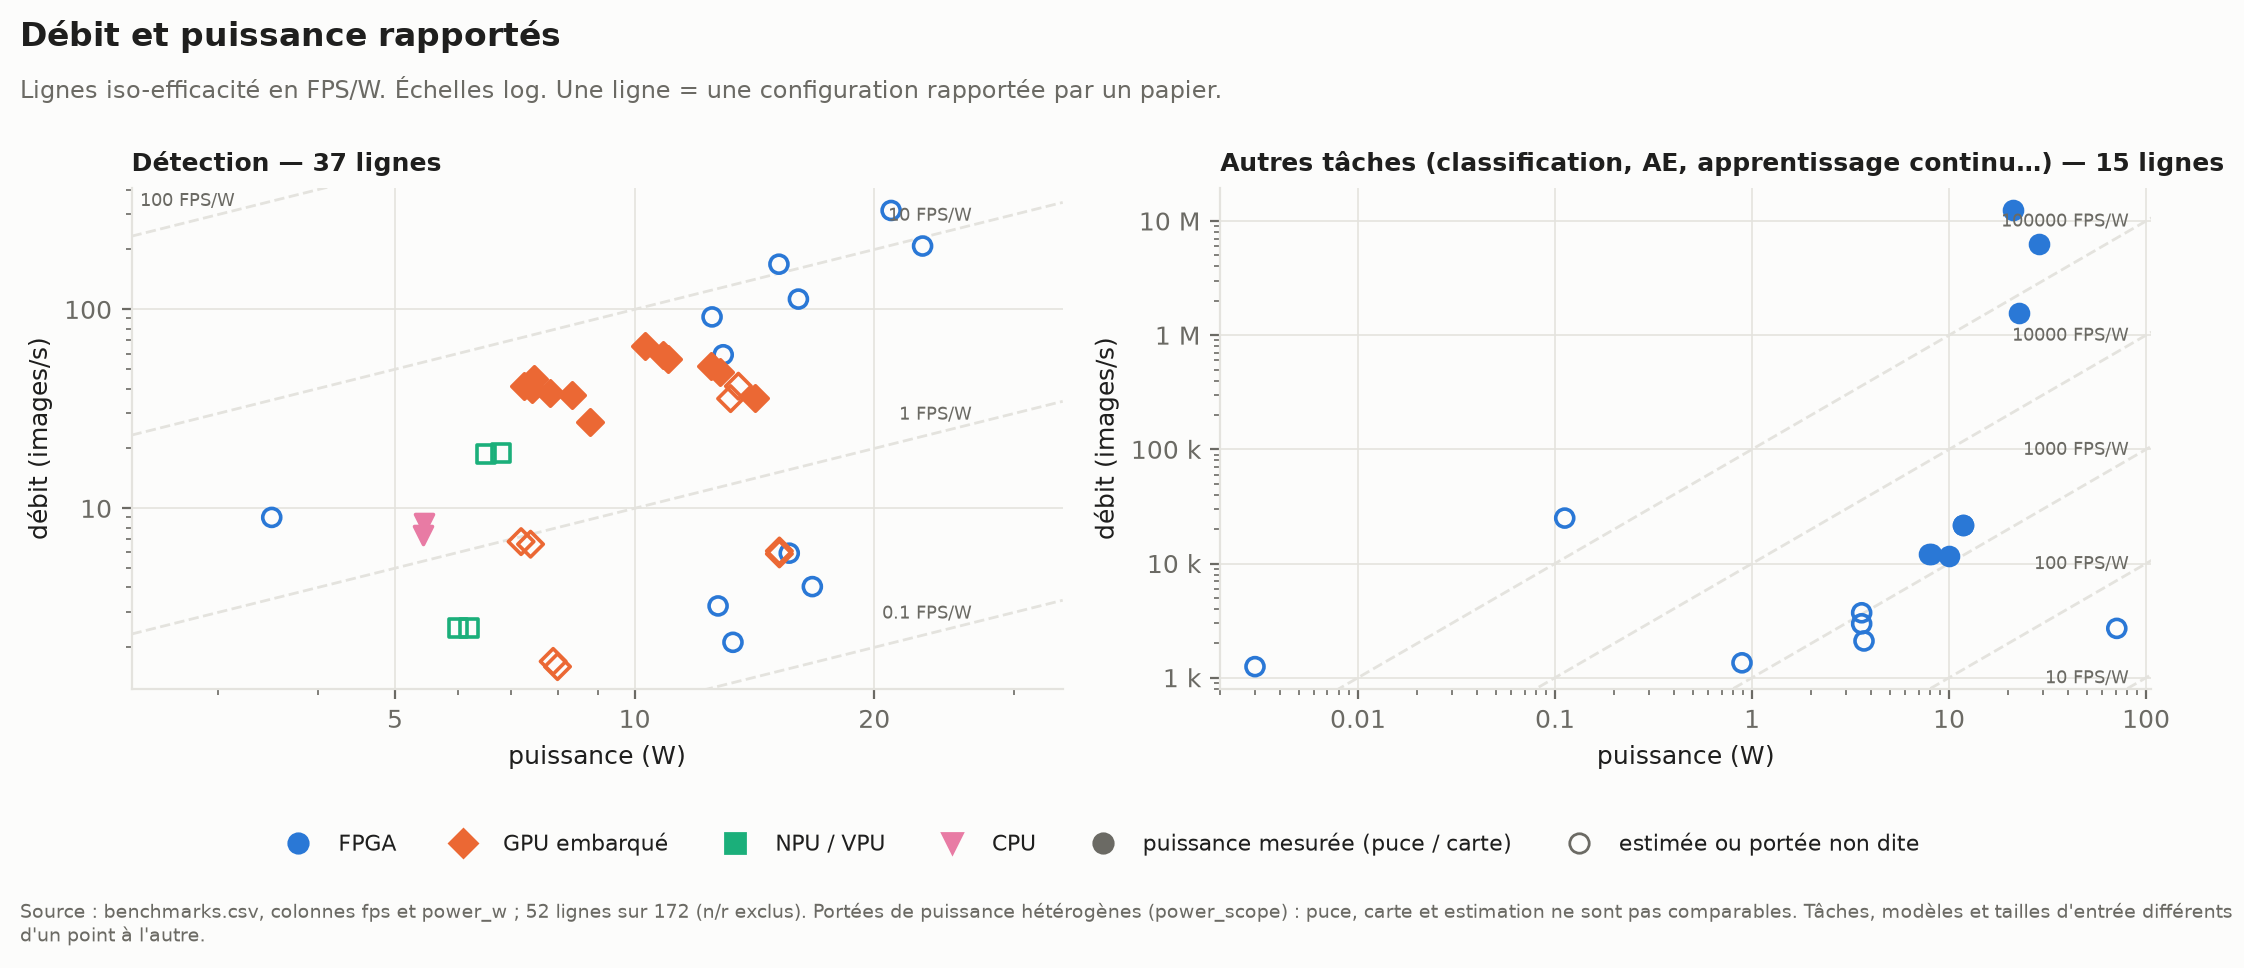
\includegraphics[width=\textwidth]{../../figures/bench_fps_power.png}
\caption{Débit et puissance rapportés, en échelles logarithmiques ; les droites
pointillées sont des lignes d'iso-efficacité en FPS/W. Figure générée par
\texttt{bin/pdb plot} à partir de \texttt{benchmarks.csv} (01/10/2026, 82 lignes sur 299).}
\label{fig:fps-power}
\end{figure}

Pour la détection (panneau de gauche, 50 lignes), ce que la figure montre :
\begin{itemize}
  \item les GPU \glslink{jetson}{Jetson} se regroupent entre 7 et 15\,\glslink{u-w}{W}, de 1,6 à 67\,images par seconde.
    Les points pleins sont les \glslink{orin-nano}{Orin Nano} et \glslink{orin-nx}{Orin NX} de Rey et al., mesurés par télémétrie
    embarquée \citep[Table~4]{arxiv-2502.15737-performance-analysis-you-only-look} ; les
    points creux, les \glslink{jetson-nano}{Jetson Nano} et \glslink{xavier-nx}{Xavier NX} de Feng et al., sans TensorRT et de portée
    non décrite \citep[Table~3]{2022-feng-benchmark-analysis-yolo-performance-edge} ;
  \item les FPGA s'étalent sur deux ordres de grandeur de débit (de 2,1 à 314\,\glslink{fps}{FPS}) et sur
    un ordre de grandeur de puissance (de 2 à 23\,\glslink{u-w}{W}) ;
  \item seules 7 des 23 lignes FPGA de détection ont une puissance mesurée, toutes au
    niveau de la carte : six \glslink{lp-yolo}{LP-YOLO} sur \glslink{pynq-z1}{PYNQ-Z1}, de 2,00 à 2,91\,\glslink{u-w}{W} pour 12 à 44\,\glslink{fps}{FPS}
    \citep[§V]{arxiv-2609.24757-npu-accelerator-quantized-real-time}\pp, et \glslink{codenet}{CoDeNet} sur
    \glslink{ultra96}{Ultra96}, 32,2\,\glslink{fps}{FPS} à 5,6\,\glslink{u-w}{W}
    \citep[Table~3]{arxiv-2006.08357-codenet-efficient-deployment-input-adaptive}$^{m}$.
    Les 16 autres sont estimées par Vivado ou de portée inconnue.
\end{itemize}
Ce que la figure ne permet pas : conclure qu'une famille est plus efficace qu'une autre.
Aucun couple de points ne partage à la fois le modèle, la résolution, la précision
numérique et la méthode de mesure \deduit. Les petites FPGA mesurées à 2--3\,\glslink{u-w}{W} portent des
\glslink{lp-yolo}{LP-YOLO} à 256 ou 320 pixels, filtrés sur les véhicules ; les \glslink{orin}{Orin} portent des \glslink{yolov8}{YOLOv8} à
640 pixels.

\subsection{Les comparaisons à tâche égale}

Six articles comparent une FPGA et un GPU embarqué sur le même réseau, mesurés par les
mêmes auteurs (table~\ref{tab:face-a-face}). Deux protocoles plus anciens s'y ajoutent :
fpgaConvNet face à un Tegra~X1 bridé à 76,8\,\glslink{u-mhz}{MHz} pour égaliser le budget de puissance
\citep[§3.1]{arxiv-1711.08740-fpgaconvnet-toolflow-mapping-diverse-convolutional}, et
\glslink{dac-sdc}{DAC-SDC}~2018, mesuré par les organisateurs \citep{2021-xu-dac-sdc-low-power-object}.

\begin{table}[!htbp]
\centering\footnotesize
\caption{Comparaisons FPGA contre GPU embarqué à réseau égal, dans un même article. Les
énergies marquées \deduit{} sont calculées ici (puissance divisée par le débit, ou
inverse du FPS/W publié).}
\label{tab:face-a-face}
\begin{tabularx}{\textwidth}{@{}P{2.3cm}P{2.4cm}LLP{3.2cm}@{}}
\toprule
Travail & Tâche, modèle & FPGA & GPU embarqué & Réserves \\
\midrule
\glslink{skynet}{SkyNet}\pp{} \src{Tables~5--7} & détection mono-objet, \glslink{dac-sdc}{DAC-SDC}'19 &
  \glslink{ultra96}{Ultra96}, FM9/W11 : \glslink{iou}{IoU} 0,716 ; 25,05\,\glslink{fps}{FPS} ; 7,26\,\glslink{u-w}{W} ; $\approx$\,0,29\,\glslink{u-j}{J}/image \deduit &
  \glslink{tx2}{TX2}, FP32 : \glslink{iou}{IoU} 0,731 ; 67,33\,\glslink{fps}{FPS} ; 13,50\,\glslink{u-w}{W} ; $\approx$\,0,20\,\glslink{u-j}{J}/image \deduit &
  portée \nr{} (organisateurs) ; batch~4 sur FPGA \\
Schlosser \src{Table~1} & \glslink{yolov4}{YOLOv4} 512, COCO &
  \glslink{zcu104}{ZCU104}, \glslink{dpu}{DPU} INT8 : \glslink{map}{mAP} 37,5 ; 54,42\,\glslink{u-ms}{ms} ; 23\,\glslink{u-w}{W} ; 1,31\,\glslink{fpsw}{FPS/W} &
  \glslink{agx-xavier}{AGX Xavier}, TensorRT INT8 : \glslink{map}{mAP} 38,6 ; 22,0\,\glslink{u-ms}{ms} ; 16,5\,\glslink{u-w}{W} ; 2,05\,\glslink{fpsw}{FPS/W} &
  carte au multimètre des deux côtés ; post-traitement optimisé sur \glslink{dpu}{DPU}, en Python sur
  \glslink{jetson}{Jetson} \\
SATAY \src{Table~IV}$^{m}$ & \glslink{yolov5n}{YOLOv5n} 640 & \glslink{zcu104}{ZCU104} : 317\,\glslink{u-mj}{mJ} & \glslink{tx2}{TX2} : 277\,\glslink{u-mj}{mJ} &
  méthode \nr ; en 320, \glslink{tx2}{TX2} 70,7\,\glslink{u-mj}{mJ} contre 117,5 à 431\,\glslink{u-mj}{mJ} \\
Castelino \src{Table~VI, §IV-B}$^{m}$ & \glslink{cae}{CAE} d'anomalies, images hyperspectrales &
  \glslink{zcu104}{ZCU104}, \glslink{dpu}{DPU} INT8 : \glslink{f1}{F1} 92,77 ; 4,0\,\glslink{u-ms}{ms} ; 5,38\,\glslink{u-w}{W} ; 21,52\,\glslink{u-mj}{mJ} &
  \glslink{xavier-nx}{Xavier NX} 10\,\glslink{u-w}{W}, TensorRT INT8 : \glslink{f1}{F1} 95,29 ; 10,36\,\glslink{u-ms}{ms} ; 7,6\,\glslink{u-w}{W} ; $\approx$\,79\,\glslink{u-mj}{mJ}
  \deduit & puce (PMBus) contre jtop ; \glslink{jetson}{Jetson} bridée \\
\glslink{f-lic}{F-LIC} \src{Fig.~6}$^{m}$ & compression apprise, encodage 720p & \glslink{vcu118}{VCU118} : 1,41\,\glslink{u-j}{J} &
  \glslink{xavier-nx}{Xavier NX} : 1,43\,\glslink{u-j}{J} & méthode \nr ; grosse FPGA \\
\glslink{chameleon}{Chameleon} \src{Table~VI}$^{m}$ & apprentissage continu, \glslink{mobilenet}{MobileNetV1}, CORe50 &
  \glslink{zcu102}{ZCU102}, FP16 : 413\,\glslink{u-ms}{ms} ; 1,22\,\glslink{u-j}{J} par image &
  \glslink{jetson-nano}{Jetson Nano} : 33\,\glslink{u-ms}{ms} ; 0,31\,\glslink{u-j}{J} par image & batch~1 contre 8 ; méthode \nr \\
\bottomrule
\end{tabularx}
\end{table}

Les sources : \citet{arxiv-1909.09709-skynet-hardware-efficient-method-object}\pp,
\citet{arxiv-2304.11580-framework-benchmarking-real-time-embedded},
\citet{2023-montgomerie-corcoran-satay-streaming-architecture-toolflow-accelerating},
\citet{arxiv-2407.17647-energy-efficient-artefact-detection-accelerator},
\citet{2022-sun-f-lic-fpga-learned-image} et
\citet{2024-aggarwal-chameleon-dual-memory-replay-online}. Ce que la table montre :
\begin{itemize}
  \item sur les trois détecteurs, le GPU embarqué est au moins aussi sobre par image.
    Chez \glslink{skynet}{SkyNet}\pp{} et Schlosser et al., il est aussi plus rapide et plus précis, y
    compris en INT8 des deux côtés : le \glslink{yolov4}{YOLOv4} de Schlosser et al. tient 2,05\,\glslink{fpsw}{FPS/W} sur
    \glslink{agx-xavier}{AGX Xavier} contre 1,31 sur \glslink{zcu104}{ZCU104}. SATAY est en moyenne 3,6 fois plus rapide que la
    \glslink{tx2}{TX2} \src{§VI-B}, mais pas plus sobre ;
  \item la seule comparaison favorable au FPGA est celle de Castelino et al. : 2,6 fois
    moins de latence et 3,6 fois moins d'énergie que la \glslink{xavier-nx}{Xavier NX} \src{§IV-B}. Mais les
    portées diffèrent (rails de la puce contre jtop), la \glslink{jetson}{Jetson} est bridée à 10\,\glslink{u-w}{W}, et le
    FPGA perd 2,5 points de \glslink{f1}{F1}. Il s'agit d'un \glslink{ae}{autoencodeur}, pas d'un détecteur ;
  \item \glslink{f-lic}{F-LIC} est à parité d'énergie avec la \glslink{xavier-nx}{Xavier NX}, sur une FPGA de centre de calcul ;
    \glslink{chameleon}{Chameleon} est quatre fois moins sobre que la \glslink{jetson-nano}{Jetson Nano} \deduit.
\end{itemize}
Aucune de ces comparaisons n'oppose une FPGA embarquée à une \glslink{orin}{Jetson Orin} \deduit.

\subsection{Énergie par inférence : des ordres de grandeur}

\begin{table}[!htbp]
\centering\footnotesize
\caption{Énergie par inférence (ou par événement d'apprentissage) rapportée dans le corpus.
Tâches, modèles et portées diffèrent : ces valeurs donnent des ordres de grandeur, pas un
classement. Les valeurs marquées \deduit{} sont calculées ici à partir de la puissance et
du débit publiés.}
\label{tab:energie}
\begin{tabularx}{\textwidth}{@{}P{2.6cm}LP{2.4cm}rP{2.8cm}@{}}
\toprule
Travail & Tâche, modèle & Plateforme & Énergie & Portée, source \\
\midrule
\glslink{tinyissimoyolo}{TinyissimoYOLO} & détection 88$\times$88, 3 classes & MAX78000 & 196\,\glslink{u-uj}{µJ} & MCU seul, §III \\
\glslink{tinyissimoyolo}{TinyissimoYOLO} & idem & Apollo4b & 6,1\,\glslink{u-mj}{mJ} & MCU seul, §III \\
Manjunath & encodeur \glslink{ae}{AE} 120$\times$120 & \glslink{artix7}{Artix-7} & 0,25\,\glslink{u-mj}{mJ} & estimée (Vivado), Table~5 \\
\glslink{imagehd}{ImageHD} & clustering continu, CIFAR-10 & \glslink{zcu104}{ZCU104} & 0,97\,\glslink{u-mj}{mJ} & estimée (Vitis), Table~VII \\
MLPerf Tiny\pp & classification CIFAR-10, FINN W1A1 & \glslink{pynq-z2}{Pynq-Z2} & 2,5\,\glslink{u-mj}{mJ} & appareil sous
  test (Joulescope), Table~5 \\
Castelino & \glslink{cae}{CAE} d'anomalies, hyperspectral & \glslink{zcu104}{ZCU104} & 21,5\,\glslink{u-mj}{mJ} & puce (PMBus), §IV-B \\
Castelino (baseline) & idem & \glslink{xavier-nx}{Xavier NX} (10\,\glslink{u-w}{W}) & $\approx$\,79\,\glslink{u-mj}{mJ} & jtop, Table~VI
  \deduit \\
\glslink{lp-yolo}{LP-YOLO Slim}\pp & détection de véhicules, 256 & \glslink{pynq-z1}{PYNQ-Z1} & $\approx$\,82\,\glslink{u-mj}{mJ} & carte
  (rail 12\,V), §V-D \deduit \\
Rey & \glslink{yolov8n}{YOLOv8n} 640 INT8 & \glslink{orin-nx}{Orin NX} & 179\,\glslink{u-mj}{mJ} & télémétrie, Table~4 \\
Rey & \glslink{yolov8n}{YOLOv8n} 640 INT8 & \glslink{orin-nano}{Orin Nano} & 185\,\glslink{u-mj}{mJ} & télémétrie, Table~4 \\
\glslink{skynet}{SkyNet}\pp & détection mono-objet & \glslink{tx2}{TX2} / \glslink{ultra96}{Ultra96} & $\approx$\,200 / 290\,\glslink{u-mj}{mJ} &
  \nr, Tables~5--6 \deduit \\
Karki\pp & \glslink{yolov26n}{YOLOv26n} 416 INT8 & \glslink{zcu104}{ZCU104} & $\approx$\,257\,\glslink{u-mj}{mJ} & estimée (Vivado),
  §IV-C, Table~III \deduit$^{m}$ \\
SATAY & \glslink{yolov5n}{YOLOv5n} 640 & \glslink{zcu104}{ZCU104} & 317\,\glslink{u-mj}{mJ} & non décrite, Table~IV$^{m}$ \\
SATAY (baseline) & \glslink{yolov5n}{YOLOv5n} 640 & \glslink{tx2}{Jetson TX2} & 277\,\glslink{u-mj}{mJ} & non décrite, Table~IV$^{m}$ \\
Schlosser & \glslink{yolov4}{YOLOv4} 512 INT8 & \glslink{agx-xavier}{AGX Xavier} / \glslink{zcu104}{ZCU104} & $\approx$\,0,49 / 0,76\,\glslink{u-j}{J} & carte,
  Table~1 \deduit \\
Alqahtani\pp & \glslink{yolov8}{YOLOv8} n à m, service web & \glslink{orin-nano}{Orin Nano} & 0,47 à 0,79\,\glslink{u-j}{J} & carte, repos
  soustrait, §IV \deduit$^{m}$ \\
\glslink{f-lic}{F-LIC} & encodage 720p (compression apprise) & \glslink{vcu118}{VCU118} & 1,41\,\glslink{u-j}{J} & non décrite, Fig.~6$^{m}$ \\
\glslink{f-lic}{F-LIC} (baseline) & idem & \glslink{xavier-nx}{Xavier NX} & 1,43\,\glslink{u-j}{J} & non décrite, Fig.~6$^{m}$ \\
\glslink{chameleon}{Chameleon} & image d'apprentissage continu & \glslink{zcu102}{ZCU102} / \glslink{jetson-nano}{Jetson Nano} & 1,22 / 0,31\,\glslink{u-j}{J} & non
  décrite, Table~VI$^{m}$ \\
O-FSCIL & ajout d'une classe (5 exemples) & \glslink{gap9}{GAP9} & 11,35\,\glslink{u-mj}{mJ} & non décrite, Table~IV \\
\glslink{qlr-cl}{QLR-CL} & événement d'apprentissage ($l = 27$) & \glslink{vega}{VEGA} & 0,13\,\glslink{u-j}{J} & puce, Table~IV \\
\glslink{qlr-cl}{QLR-CL} & idem & \glslink{stm32l4}{STM32L4} & 4,80\,\glslink{u-j}{J} & Table~IV \\
\bottomrule
\end{tabularx}
\end{table}

Sources des lignes nouvelles : MLPerf Tiny
\citep[Table~5]{arxiv-2206.11791-open-source-fpga-ml-codesign}\pp ; \glslink{lp-yolo}{LP-YOLO Slim}, 35,66\,\glslink{fps}{FPS}
à 2,91\,\glslink{u-w}{W}, soit 12,25\,\glslink{fpsw}{FPS/W}
\citep[§V-D]{arxiv-2609.24757-npu-accelerator-quantized-real-time}\pp ; Karki et al.,
34,05\,\glslink{fps}{FPS} de bout en bout et 8,760\,\glslink{u-w}{W} estimés par Vivado
\citep[§IV-C, Table~III]{arxiv-2607.13106-no-attention-no-problem-dpu}\pp ; Alqahtani et
al., 0,13 à 0,22\,mWh par requête, latence de service web comprise
\citep[§IV]{arxiv-2409.16808-comprehensive-evaluation-deep-learning-object}\pp. Pour
mémoire, le \glslink{yolov3-tiny}{YOLOv3-tiny} de Zhai et al. donnerait environ 136\,\glslink{u-mj}{mJ} par image (12,51\,\glslink{u-w}{W}
divisés par 91,65\,\glslink{fps}{FPS}, \citealp[Table~8]{2023-zhai-fpga-vehicle-detection-tracking-accelerator}),
de portée non décrite. Ces calculs sont les nôtres \deduit.

La table ne classe pas les plateformes. Trois écarts la dominent : la taille du réseau
(de 88$\times$88 pixels sur MCU à 640 sur \glslink{jetson}{Jetson}), la portée de la mesure (outil, puce,
carte, carte moins le repos), et le périmètre de l'inférence (noyau seul, bout en bout,
service web). Le seul détecteur sur petite FPGA mesuré à la carte (\glslink{lp-yolo}{LP-YOLO}, 82\,\glslink{u-mj}{mJ}) et
les \glslink{orin}{Orin} mesurés par télémétrie (179 à 185\,\glslink{u-mj}{mJ}) diffèrent sur ces trois points à la fois.

\subsection{Pourquoi la comparaison reste ouverte}

Pour comparer honnêtement un FPGA embarqué, une \glslink{jetson}{Jetson} et un MCU, il faudrait, sur un même
réseau :
\begin{itemize}
  \item la même précision numérique et le même batch ;
  \item une précision mesurée sur chaque cible ;
  \item une latence de bout en bout, post-traitement compris ;
  \item une puissance de puce et de carte, avec le repos mesuré.
\end{itemize}
Le protocole de \citet{arxiv-2304.11580-framework-benchmarking-real-time-embedded} est le
plus proche de cette grille dans le corpus : même \glslink{yolov4}{YOLOv4}, \glslink{map}{mAP} mesurée sur la cible par un
hôte séparé, puissance de carte absolue et relative (repos soustrait), quatre modes de
puissance \glslink{jetson}{Jetson} \src{§3, §4.1, §4.4}. Il lui manque l'égalité du post-traitement et une cible
récente, et il ne porte que sur un modèle. MLPerf Tiny fixe aussi un protocole (latence à
batch~1, énergie au Joulescope), mais l'article ne compare aucune autre plateforme
\citep[§1, §4.4]{arxiv-2206.11791-open-source-fpga-ml-codesign}\pp. Les meilleures
baselines \glslink{jetson}{Jetson} récentes (Rey, Alqahtani\pp) n'ont pas de FPGA. Les travaux FPGA récents
se comparent à des \glslink{jetson}{Jetson} anciennes ou bridées (SATAY, \glslink{skynet}{SkyNet}\pp, Castelino), à un GPU de
bureau \citep[Table~10]{2026-fata-low-cost-fpga-enhanced-cnn}, ou à rien (Karki\pp, \glslink{lp-yolo}{LP-YOLO}\pp). Aucun article du corpus ne met une FPGA
embarquée et une \glslink{orin}{Jetson Orin}, ni une FPGA et un MCU, dans un même banc d'essai.

% Section commune : autoencodeurs sur FPGA (et plateformes voisines)
\section{Autoencodeurs sur FPGA}
\label{sec:autoencodeurs}

La bibliographie de départ supposait que les autoencodeurs (AE) sur FPGA étaient surtout
étudiés sur des séries temporelles et en physique des particules, et peu sur des images.
Les 11 fiches de l'axe permettent de préciser ce constat.

\subsection{Physique des particules et signaux : la très faible latence}

\citet{arxiv-2108.03986-autoencoders-fpgas-real-time-unsupervised} placent des AE et VAE
au déclenchement de premier niveau du LHC, pour sélectionner des collisions anormales sans
hypothèse sur la nouvelle physique. Trois choix sont transposables à d'autres domaines :
\begin{itemize}
  \item le score d'anomalie (erreur quadratique) est calculé sur la puce, par une couche
    ajoutée à hls4ml \src{§IV} ;
  \item le VAE est réduit à son encodeur : le score s'obtient à partir de la divergence de
    Kullback-Leibler ($D_{KL}$) calculée sur $(\mu, \sigma)$, ce qui supprime
    l'échantillonnage et le décodeur \src{§IV} ;
  \item le choix entre QAT et PTQ se fait selon la stabilité du score d'anomalie, et non
    selon la perte d'entraînement \src{§VI}.
\end{itemize}
Le VAE dense (encodeur seul) tient en 80\,ns sur VU9P ; le seul AE convolutif, sur une
entrée de 19$\times$3 valeurs, prend 47\,\% des LUT et est rejeté \src{Table~III}. Ces
chiffres sont des estimations de Vivado HLS ; une seule validation sur carte est faite, et
elle est qualitative \src{§VII}.

Deux autres travaux restent sur des signaux :
\begin{itemize}
  \item \citet{arxiv-2602.15751-enabling-low-latency-machine-learning} compressent des
    impulsions de calorimètre (32 échantillons en 2 valeurs) sur un PolarFire durci : 25\,ns
    de latence en version \enquote{nano}, sans bloc mathématique \src{§5.2}$^{m}$. La
    puissance est estimée par l'outil ;
  \item \citet{2024-que-low-latency-variational-autoencoder-fpgas} sont les seuls à
    échantillonner en matériel (générateur Mersenne Twister suivi d'une transformée de
    Box-Muller), avec un latent de dimension~1, sur des séries d'ondes gravitationnelles
    \src{§III}. Une inférence dure 17 cycles (85\,ns) ; les \enquote{5,6\,ns} mis en avant
    sont un débit inverse amorti sur 10\,000 inférences \src{§IV-E}. La puissance est
    estimée par Vivado \src{§IV-E}.
\end{itemize}
Enfin, \citet{2024-campos-end-end-codesign-hessian-aware} quantifient un encodeur de
compression de données de calorimètre (ECON-AE), dont seul l'encodeur est synthétisé
\src{§7, Table~3}.

\subsection{Images : compression apprise et encodeurs}

\paragraph{Compression apprise sur grosse FPGA.} F-LIC
\citep{2022-sun-f-lic-fpga-learned-image} implante un codec d'images appris (VAE avec
hyper-prior) en virgule fixe 8~bits sur VCU118. Il encode du 720p à 40,69\,FPS et du 1080p
à 19,15\,FPS, avec un PSNR de 29,94\,dB à 0,2542\,bpp \src{Fig.~6}$^{m}$. Deux techniques
sont réutilisables pour un décodeur :
\begin{itemize}
  \item deux poids partagent un même DSP (\enquote{casDSP}) ;
  \item la déconvolution saute les zéros insérés par le stride.
\end{itemize}
Deux limites : le codage entropique tourne sur le PC hôte \src{Fig.~1}, et l'encodeur 720p
occupe 4\,146 DSP. L'énergie par image est comparable à celle d'une Jetson Xavier NX (1,41
contre 1,43\,J en encodage 720p), pas meilleure, et la méthode de mesure n'est pas décrite
\src{Fig.~6}.

\paragraph{Compression à bord, sur VPU.} La mission Φ-Sat-2
\citep{2023-guerrisi-artificial-intelligence-board-image-compression} compresse les images
par un AE convolutif d'un facteur 8 fixe, sans codage entropique \src{§II-A}. L'encodeur
tourne à bord sur une VPU Myriad~2, pas sur un FPGA : 10,92\,s par acquisition pour
1,4\,W, contre 0,95\,s sur un GPU GTX~1650 \src{Table~V}$^{m}$. Le passage à la VPU ne
coûte presque rien en qualité : SSIM de 0,9647 contre 0,9651 \src{§III-B--C}.

\paragraph{Encodeurs d'images sur petite FPGA.}
\citet{2021-manjunath-energy-efficient-edgeai-autoencoder-accelerator} ternarisent
l'encodeur convolutif d'un agent d'apprentissage par renforcement (entrée 120$\times$120
RGB, simulateur) et l'implantent en Verilog sur Artix-7. En 32~bits et 64~PE, une image
coûte 0,8\,ms et 0,25\,mJ \src{Table~5}. La puissance est estimée par Vivado
\src{§VIII-A}, et le décodeur n'est pas implanté.
\citet{arxiv-2301.07050-energy-efficient-reconfigurable-autoencoder-implementation}\pp{}
débruitent MNIST sur XCZU7EV (2,91\,ms, 5,93\,W \enquote{on-chip}). C'est la seule ligne
de \texttt{benchmarks.csv} en confiance \emph{low} : l'\enquote{accuracy} d'un débruiteur
n'est pas définie, et le tableau comparatif est physiquement incohérent \src{Table~II}.

\subsection{Détection d'anomalies sur petite FPGA : des signaux, pas des images}

\begin{itemize}
  \item \citet{2022-malviya-edge-compatible-convolutional-autoencoder-implemented}
    détectent des anomalies de vibrations d'hélicoptère, encodées en scalogrammes
    64$\times$64, avec un AE convolutif de 8\,755 paramètres sur PYNQ-Z2. Encodeur et
    décodeur sont dans deux bitstreams séparés (40\,403 et 38\,169 LUT), pour 2,1 + 3,8\,ms
    \src{Table~4, §IV-B}$^{m}$. La précision est remesurée sur le FPGA et baisse (85,02\,\%
    contre 88,8\,\% sur CPU) en virgule fixe 23~bits \src{§IV-B}.
  \item \citet{2019-tsukada-neural-network-device-learning-anomaly} (ONLAD) apprennent en
    ligne un AE à une couche cachée par OS-ELM (voir
    section~\ref{sec:cl-fpga}). Leurs données sont tabulaires ou des images aplaties.
  \item \citet{2019-coutinho-deep-neural-network-hardware-implementation} : malgré le
    titre, l'\enquote{autoencodeur empilé} n'est qu'un classifieur MLP sur MNIST, sans
    reconstruction \src{§III-A, §V-D}. Leur comparaison met une puissance dynamique de
    quelques mW face à des puissances totales \src{Tables~16--17}.
\end{itemize}

\subsection{Bilan}

\begin{table}[!htbp]
\centering\footnotesize
\caption{Autoencodeurs du corpus : donnée traitée, partie implantée et type de mesure.}
\label{tab:ae}
\begin{tabularx}{\textwidth}{@{}P{2.6cm}P{3.1cm}LP{2cm}P{2.4cm}@{}}
\toprule
Travail & Donnée & Partie en matériel & Puce & Puissance \\
\midrule
AE du LHC\,\textsuperscript{a} & tabulaire 19$\times$3 & AE complet ; VAE encodeur seul & VU9P & non mesurée \\
PicoCal\,\textsuperscript{b} & impulsions 1D & encodeur & PolarFire & estimée \\
VAE de Que\,\textsuperscript{c} & séries temporelles & VAE complet (latent 1) & U250, Z7045 & estimée \\
ECON-AE\,\textsuperscript{d} & calorimètre & encodeur & \nr{} (voir fiche) & non mesurée \\
F-LIC\,\textsuperscript{e} & images 720p et 1080p & VAE hyper-prior, sans codage entropique & VCU118 & méthode non décrite \\
Φ-Sat-2\,\textsuperscript{f} & images satellite & encodeur & VPU (pas de FPGA) & méthode non décrite \\
Manjunath\,\textsuperscript{g} & images 120$\times$120 (simulateur) & encodeur & Artix-7 & estimée \\
CAE débruiteur\,\textsuperscript{h} & MNIST bruité & AE complet & XCZU7EV & méthode non décrite \\
Malviya\,\textsuperscript{i} & vibrations en scalogrammes & AE, 2 bitstreams & XC7Z020 & méthode non décrite \\
ONLAD\,\textsuperscript{j} & tabulaire, MNIST aplati & AE OS-ELM + apprentissage & XC7Z020 & carte (3,1\,W) \\
SSAE\,\textsuperscript{k} & MNIST & MLP (encodeurs empilés) & XC6VLX240T & dynamique \\
\bottomrule
\end{tabularx}

\smallskip\raggedright\footnotesize
\textsuperscript{a}\,\citet{arxiv-2108.03986-autoencoders-fpgas-real-time-unsupervised} ;
\textsuperscript{b}\,\citet{arxiv-2602.15751-enabling-low-latency-machine-learning} ;
\textsuperscript{c}\,\citet{2024-que-low-latency-variational-autoencoder-fpgas} ;
\textsuperscript{d}\,\citet{2024-campos-end-end-codesign-hessian-aware} ;
\textsuperscript{e}\,\citet{2022-sun-f-lic-fpga-learned-image} ;
\textsuperscript{f}\,\citet{2023-guerrisi-artificial-intelligence-board-image-compression} ;
\textsuperscript{g}\,\citet{2021-manjunath-energy-efficient-edgeai-autoencoder-accelerator} ;
\textsuperscript{h}\,\citet{arxiv-2301.07050-energy-efficient-reconfigurable-autoencoder-implementation}\pp ;
\textsuperscript{i}\,\citet{2022-malviya-edge-compatible-convolutional-autoencoder-implemented} ;
\textsuperscript{j}\,\citet{2019-tsukada-neural-network-device-learning-anomaly} ;
\textsuperscript{k}\,\citet{2019-coutinho-deep-neural-network-hardware-implementation}.
\end{table}

Trois constats se dégagent du tableau~\ref{tab:ae} :
\begin{itemize}
  \item \textbf{l'image est traitée}, mais par la compression sur grosse FPGA (F-LIC), sur
    VPU (Φ-Sat-2), ou à petite échelle sur petite FPGA (Manjunath,
    arxiv-2301.07050\pp) ;
  \item \textbf{aucun article ne détecte d'anomalies visuelles par AE sur FPGA} : les AE
    d'anomalie portent sur des signaux ou des données tabulaires ;
  \item \textbf{l'AE complet sur une petite puce reste coûteux} : au 26/09, on implantait
    l'encodeur seul, ou l'on coupait le réseau en deux bitstreams. Depuis, deux articles
    implantent encodeur et décodeur sur une UltraScale+ (CAE d'artefacts hyperspectraux sur
    la DPU d'une ZCU104, \citealp{arxiv-2407.17647-energy-efficient-artefact-detection-accelerator} ;
    compression apprise sur ZCU102,
    \citealp{arxiv-2503.04832-lightweight-embedded-fpga-deployment-learned}). Le coût des
    déconvolutions sur une puce de la taille d'une KV260 reste non mesuré.
\end{itemize}
Le survey d'anomalie visuelle industrielle de
\citet{2023-cui-survey-unsupervised-anomaly-detection-algorithms}, pas encore fiché, dira
quels modèles d'anomalie visuelle seraient les candidats à porter.

% Section commune : apprentissage embarqué et continu sur FPGA
\section{Apprentissage embarqué et continu sur FPGA}
\label{sec:cl-fpga}

Un modèle figé ne s'adapte pas à la dérive des données. L'apprentissage sur l'appareil y
répond, mais la rétropropagation coûte cher en mémoire et en énergie. Les deux seuls
apprentissages sur FPGA du corpus l'évitent.

\paragraph{ONLAD : apprentissage séquentiel sans rétropropagation.}
\citet{2019-tsukada-neural-network-device-learning-anomaly} entraînent en ligne un AE à une
couche cachée par OS-ELM :
\begin{itemize}
  \item les poids d'entrée sont aléatoires et figés, et seuls les poids de sortie sont mis
    à jour par moindres carrés récursifs \src{§2.2, §3.3} ;
  \item à batch~1, la seule inversion matricielle devient une division scalaire, sans
    changer la solution \src{§3.1} ;
  \item un facteur d'oubli léger gère la dérive : l'AUC passe de 0,55--0,59 sans oubli à
    0,78--0,90 sous dérive simulée \src{Table~5}.
\end{itemize}
Le cœur (Vivado HLS, virgule fixe 32~bits, 100\,MHz) tourne sur PYNQ-Z1. C'est l'une des
rares mesures de carte FPGA du corpus : 3,1\,W au wattmètre, ARM compris \src{§6.4}.
Limites : les AUC sont évaluées en TensorFlow et non sur le cœur en virgule fixe
\src{§5--6} ; la dérive est simulée par permutation de classes ; les baselines CPU et GPU,
en TensorFlow à batch~1, sont dominées par les surcoûts d'appel, ce que les auteurs
reconnaissent \src{§6.2.1}.

\paragraph{ImageHD : calcul hyperdimensionnel sur un extracteur figé.}
\citet{arxiv-2604.21280-imagehd-energy-efficient-device-continual} combinent un MobileNetV2
INT8 figé, un encodage en hypervecteurs binaires et une mémoire de clusters bornée,
fusionnée par un kMeans++ simplifié \src{§IV}. L'accélérateur streaming (Vitis HLS) tient
sur une ZCU104 à 300\,MHz : 0,27\,ms et 0,97\,mJ par image sur CIFAR-10
\src{Tables~VI--VII}. Deux réserves fortes :
\begin{itemize}
  \item la précision de clustering est très basse (0,27 sur CIFAR-10, 0,19 sur CORe50),
    alors que l'article parle d'une \enquote{strong accuracy} \src{Table~VI, §IX} ;
  \item latence et puissance du FPGA viennent de l'analyseur de Vitis, c'est-à-dire d'une
    estimation, alors que CPU et GPU sont mesurés (powertop, nvidia-smi). Les gains de
    258$\times$ à 383$\times$ en énergie mélangent estimation et mesure \src{§VII-D}.
\end{itemize}

\paragraph{Références hors FPGA.} Deux travaux fixent des ordres de grandeur qu'un
apprentissage continu sur FPGA devrait battre ou justifier :
\begin{itemize}
  \item QLR-CL sur VEGA, un ASIC PULP 22\,nm : 62\,mW de puce
    \citep[§V-D]{arxiv-2110.10486-tinyml-platform-device-continual-learning} ;
  \item O-FSCIL sur le MCU GAP9 : 11 à 23\,mJ par nouvelle classe
    \citep[Table~IV]{arxiv-2403.07851-12-mj-per-class-device}.
\end{itemize}
\ifcomplete Tous deux sont détaillés en section~\ref{sec:cl-mcu}.\else Tous deux sont détaillés dans la version complète de l'état de l'art.\fi La seule
rétropropagation embarquée du corpus (la queue d'un MobileNet-V1, en FP32) tourne sur VEGA,
pas sur un FPGA
\citep[§IV-B]{arxiv-2110.10486-tinyml-platform-device-continual-learning}. Venieris et al.
jugeaient déjà l'entraînement sur FPGA \enquote{à peine exploré} en 2018
\citep[§3.2]{2018-venieris-toolflows-mapping-convolutional-neural-networks}.

\paragraph{Ce qui manque.} Toutes les fiches d'apprentissage continu font de la
classification ou du clustering ; \texttt{benchmarks.csv} n'a aucune ligne qui croise
détection et apprentissage continu. Deux questions restent ouvertes dans le corpus :
\begin{itemize}
  \item une rétropropagation de la queue d'un réseau sur SoC FPGA, avec l'étage figé en
    logique programmable ;
  \item l'incrémental de classes en détection.
\end{itemize}

% Section propre à la version complète : apprentissage continu sur MCU et ASIC
\section{Apprentissage continu sur microcontrôleurs et ASIC}
\label{sec:cl-mcu}

\paragraph{Replay latent quantifié sur ASIC PULP (QLR-CL).}
\citet{arxiv-2110.10486-tinyml-platform-device-continual-learning} découpent un MobileNet-V1
(entrée 128$\times$128) en deux étages \src{§III-C} :
\begin{itemize}
  \item un \emph{étage figé}, quantifié en INT8 ;
  \item un \emph{étage adaptatif}, réentraîné en FP32 par rétropropagation, sur un mélange
    de nouvelles images et d'activations intermédiaires stockées en 8~bits (\emph{latent
    replays}).
\end{itemize}
Sur Core50, stocker ces activations en UINT-8 ne coûte que 0,26 point face au FP32
\src{§V-B}. En dessous de 6~bits, l'apprentissage ne converge plus. Sur VEGA (ASIC 22\,nm,
62\,mW mesurés sur la puce), un événement d'apprentissage coûte 2,07\,s et 0,13\,J si seule
la dernière couche est réentraînée. Si l'on remonte à la couche~23, il faut 877\,s et
54,3\,J \src{Table~IV}. Avec le même code, VEGA est en moyenne 65 fois plus rapide et 37
fois plus économe qu'un STM32L4 \src{§V-E}. La comparaison au Snapdragon~845, elle, suppose
une enveloppe de 4\,W non mesurée \src{§V-E}.

\paragraph{Apprentissage incrémental de classes à partir de peu d'exemples, sur GAP9
(O-FSCIL).} \citet{arxiv-2403.07851-12-mj-per-class-device} figent un MobileNetV2 et
ajoutent chaque nouvelle classe sous la forme d'un prototype : la moyenne des
caractéristiques de ses 5 exemples, sans rétropropagation \src{§IV, §V-B}. Sur GAP9, en
INT8, ajouter une classe coûte 11,35\,mJ pour 62,44\,\% de précision moyenne sur
CIFAR-100. Le plus gros backbone atteint 66,51\,\% pour 22,75\,mJ \src{Tables~II et IV}.
Le titre combine deux configurations : les 68,62\,\% viennent d'un ResNet-12 FP32 sur GPU,
les 12\,mJ du plus petit modèle déployé \src{Table~II}.

\paragraph{Non encore fichés.} L'entraînement sous 256\,KB de mémoire
\citep{arxiv-2206.15472-device-training-256kb-memory}\pp{} et l'apprentissage continu sur MCU
par distillation de données \citep{arxiv-2409.07114-continual-incremental-learning-tinyml-device}
sont dans la base, mais sans fiche : ils ne sont pas exploités ici. Le survey de
\citet{arxiv-2411.01431-efficient-deep-learning-infrastructures-embedded} traite
l'apprentissage continu embarqué en une page, sans aucun chiffre système \src{§5.2}.

\paragraph{Bilan transversal.} Les cinq fiches d'apprentissage continu couvrent au plus
deux familles de plateformes chacune :
\begin{itemize}
  \item QLR-CL : ASIC et MCU ;
  \item O-FSCIL : MCU ;
  \item ImageHD : FPGA, face au CPU, au GPU et à une Jetson non optimisée ;
  \item ONLAD : FPGA, face au CPU et au GPU.
\end{itemize}
Aucun algorithme d'apprentissage continu n'est mesuré à la fois sur MCU, FPGA et Jetson.
\texttt{benchmarks.csv} n'a aucune ligne d'apprentissage continu sur Jetson.

% Section commune : analyse critique transversale
\section{Analyse critique : ce que les chiffres publiés permettent de conclure}
\label{sec:critique}

\subsection{La puissance : rarement mesurée sur la carte, presque jamais sur la puce FPGA}

Recompte de \texttt{benchmarks.csv} sur les 216 lignes mesurées sur FPGA (44 articles) :

\begin{table}[!htbp]
\centering\small
\caption{Portée de la puissance dans les lignes FPGA de \texttt{benchmarks.csv}
(01/10/2026).}
\label{tab:portee}
\begin{tabularx}{\textwidth}{@{}lrL@{}}
\toprule
Portée & Lignes & Origine \\
\midrule
\emph{board} (carte au wattmètre) & 46 & 9 articles : Zhang 2024 10, FINN 8, FINN-R 8,
  Elastic-DF 8, \glslink{lp-yolo}{LP-YOLO} 6, Schlosser 3, Zhang 2015, \glslink{onlad}{ONLAD} et \glslink{codenet}{CoDeNet} 1 chacun \\
\emph{chip} & 1 & Castelino (rails PMBus de la \glslink{zcu104}{ZCU104}) \\
\emph{board-dynamic} & 0 & --- \\
\emph{estimated} (outil) & 16 & \glslink{ef-train}{EF-Train} 6, Manjunath 4, \glslink{imagehd}{ImageHD} 3, Karki 2, Que 2024 1 \\
\emph{unspecified} & 52 & dont SATAY 14, Piyasena 16 (deux articles), Zhai 8 \\
puissance non rapportée (\nr) & 101 & --- \\
\bottomrule
\end{tabularx}
\end{table}

Un peu plus de la moitié des lignes FPGA (115 sur 216) ont une puissance, et 47
seulement une puissance mesurée, issues de 10 articles. Les 18 lignes \emph{chip} de la base viennent,
sauf une, de \glslink{orin}{Jetson Orin} (12, \citealp{arxiv-2502.15737-performance-analysis-you-only-look}),
du Raspberry~Pi~5 (2) et de l'ASIC \glslink{vega}{VEGA} (3). La seule ligne \emph{chip} FPGA est celle de
\citet[§IV-B]{arxiv-2407.17647-energy-efficient-artefact-detection-accelerator} : 5,38\,\glslink{u-w}{W}
actifs pour 4,6\,\glslink{u-w}{W} au repos. Les lignes \emph{board} ne sont plus surtout anciennes : à
côté de FINN, FINN-R, Zhang 2015 et \glslink{onlad}{ONLAD}, elles viennent de
\citet{2024-zhang-end-end-acceleration-yolo-object},
\citet{2021-alonso-elastic-df-scaling-performance-dnn} (deux Alveo, hors embarqué),
\citet{arxiv-2304.11580-framework-benchmarking-real-time-embedded} et
\citet{arxiv-2609.24757-npu-accelerator-quantized-real-time}\pp. Une seule paire puce /
carte existe sur une même FPGA, et la puce y est estimée : 7,8\,\glslink{u-w}{W} par Vivado contre
12,3\,\glslink{u-w}{W} au wattmètre sur KC705 \citep[Table~3]{2024-zhang-end-end-acceleration-yolo-object}.
Seuls Schlosser et al. donnent aussi la puissance relative, repos soustrait, que le CSV
ne reprend pas faute de ligne \emph{board-dynamic} : 7,0\,\glslink{u-w}{W} sur \glslink{zcu104}{ZCU104} pour 23\,\glslink{u-w}{W} absolus
\src{Table~1}.

Plusieurs comparaisons publiées mettent face à face des portées différentes :
\begin{itemize}
  \item une puissance dynamique de quelques mW contre des puissances totales
    \citep[Table~16]{2019-coutinho-deep-neural-network-hardware-implementation} ;
  \item la carte entière contre le CPU seul et le GPU seul
    \citep[§6.4]{2019-tsukada-neural-network-device-learning-anomaly} ;
  \item le TDP d'un Xeon pris comme puissance mesurée
    \citep[§5.2]{2015-zhang-optimizing-fpga-accelerator-design-deep} ;
  \item une estimation de l'outil contre des mesures par nvidia-smi
    \citep[§VII-D]{arxiv-2604.21280-imagehd-energy-efficient-device-continual} ;
  \item les rails PMBus de la puce contre jtop sur une \glslink{xavier-nx}{Xavier NX} bridée à 10\,\glslink{u-w}{W}
    \citep[Table~VI]{arxiv-2407.17647-energy-efficient-artefact-detection-accelerator} ;
  \item une puissance estimée par Vivado présentée comme \enquote{3x moins} que celle de
    SATAY \citep[Résumé, Table~III]{arxiv-2607.13106-no-attention-no-problem-dpu}\pp.
\end{itemize}
Le survey de \citet{2023-shuvo-efficient-acceleration-deep-learning-inference} rappelle,
dans sa partie sur les conditions de test, qu'un processeur peut afficher une très faible
consommation en omettant les accès à la mémoire externe, et qu'il faut séparer résultats
simulés et mesurés \src{§IX-I}.

\subsection{Des métriques qui flattent}

\begin{itemize}
  \item \textbf{Latence amortie} : un débit inverse présenté comme une latence
    \citep[§IV-E]{2024-que-low-latency-variational-autoencoder-fpgas}.
  \item \textbf{GOp/s par \glslink{dsp}{DSP}} : cette métrique efface les écarts de précision (de W1A8 à
    W32A32) et de carte
    \citep[Table~III]{2023-montgomerie-corcoran-satay-streaming-architecture-toolflow-accelerating}.
    Venieris et al. la jugeaient valable seulement dans une même famille de FPGA
    \citep[§3.1]{2018-venieris-toolflows-mapping-convolutional-neural-networks}. Le
    \enquote{+29\,\% face à Vitis AI} de \citet{2024-yan-fpga-yolov5-accelerator-real-time}
    est un \glslink{gopsdsp}{GOPS/DSP} face à un \glslink{yolov3}{YOLOv3} d'un autre travail, pas une mesure de Vitis AI sur la
    même carte \src{Table~2}.
  \item \textbf{Gains de surface face à des designs plus rapides} : \enquote{$-26$\,\% de
    \glslink{ff}{FF}, $-15$\,\% de \glslink{dsp}{DSP}} face à des accélérateurs de 10,5 à 62,9\,\glslink{gops}{GOPS}, pour 2,33\,\glslink{gops}{GOPS} et
    un autre modèle \citep[Table~9]{2025-kim-design-implementation-yolov2-accelerator-zynq}.
  \item \textbf{\glslink{gopsw}{GOPS/W} dynamiques} face à des \glslink{gopsw}{GOPS/W} totaux
    \citep[Table~8]{2023-zhai-fpga-vehicle-detection-tracking-accelerator}.
  \item \textbf{\glslink{gops}{GOPS} projetés} sur un FPGA hypothétique, comparés à des \glslink{gops}{GOPS} mesurés
    \citep[Tables~16--17]{2019-coutinho-deep-neural-network-hardware-implementation}.
  \item \textbf{GOp/s seul}, sans \glslink{fps}{FPS}, pour un détecteur
    \citep[Table~5]{arxiv-1809.04570-finn-r-end-end-deep} ; \enquote{10,65x} en GOp/s
    entre des UNet de tailles différentes, à \glslink{fps}{FPS} voisins
    \citep[§V-D]{arxiv-2403.18921-smof-streaming-modern-cnns-fpgas}\pp.
  \item \textbf{Gains face à un CPU ou un GPU de bureau}, de portée de puissance non dite :
    \enquote{70x / 37x}, alors que le GPU fait 44,64\,\glslink{fps}{FPS} contre 24,3 sur la \glslink{kv260}{KV260}
    \citep[Table~10]{2026-fata-low-cost-fpga-enhanced-cnn} ; gains d'énergie de 258 à
    383 fois qui mêlent une estimation FPGA et des mesures CPU et GPU
    \citep[Table~VII]{arxiv-2604.21280-imagehd-energy-efficient-device-continual}.
  \item \textbf{Conclusion contredite par son propre tableau} : 2,6\,\glslink{fpsw}{FPS/W} présentés comme
    efficaces, moins que quatre des cinq travaux cités
    \citep[§IV-B, Table~I]{arxiv-2507.18174-real-time-object-detection-classification}.
  \item \textbf{Chiffres incohérents entre résumé et texte} : 35x contre 58x
    \citep[§I-B, §IV-C]{arxiv-2402.09780-tinycl-efficient-hardware-architecture-continual}\pp ;
    perte de précision de $\approx$\,5\,\% contre $\approx$\,7\,\%
    \citep[Résumé, §IV-B]{arxiv-2607.13106-no-attention-no-problem-dpu}\pp.
  \item \textbf{Précisions non comparables} : \glslink{iou}{IoU} d'un seul objet (\glslink{dac-sdc}{DAC-SDC}, \glslink{skynet}{SkyNet}\pp), \glslink{ap}{AP}
    à une classe (Zhai), \enquote{accuracy} sur 72 images (Al Amin), \enquote{accuracy}
    non définie d'un débruiteur (arxiv-2301.07050\pp, seule ligne en confiance \emph{low}),
    \glslink{map}{mAP} sur des véhicules filtrés de VOC (\glslink{lp-yolo}{LP-YOLO}\pp), \glslink{map}{mAP} sur un jeu privé à une cible
    \citep[Table~4]{arxiv-2502.15737-performance-analysis-you-only-look}.
\end{itemize}
Le recompte confirme cette dispersion. Les 87 lignes FPGA de détection (17 articles)
emploient 14 libellés de précision différents, et 12 n'ont aucune précision. Seules 22
portent une précision sur COCO, dont 14 pour SATAY, quantification simulée par ONNX
Runtime ; six d'entre elles seulement (Schlosser, Karki\pp) sont mesurées sur la carte de
façon établie. Sur les 216 lignes FPGA, le \glslink{fps}{FPS} manque 132 fois, la latence 88 fois, la
puissance 101 fois et la précision 48 fois. Shuvo et al. le formulent ainsi : \enquote{EI requires a universal and
comprehensive set of quality metrics to execute meaningful comparisons of DL models,
optimization algorithms, and hardware platforms} \src{§XIV-C}. La grille de Venieris et al.
(débit, latence à batch~1, ressources, puissance, précision, mémoire) existe depuis 2018 ;
aucune fiche du corpus ne la reprend en entier.

\subsection{La précision est rarement remesurée sur la cible}

Quantifier et compiler un réseau change sa précision, et la plupart des articles ne la
remesurent pas sur la carte :
\begin{itemize}
  \item \glslink{ap}{AP} identique en FP32 et en INT16 à trois décimales
    \citep[Table~8]{2023-zhai-fpga-vehicle-detection-tracking-accelerator} ;
  \item quantification simulée par ONNX Runtime
    \citep[§IV-A]{2023-montgomerie-corcoran-satay-streaming-architecture-toolflow-accelerating} ;
  \item comparaison au C++ généré, pas au FPGA
    \citep[§8]{arxiv-2101.05108-fast-convolutional-neural-networks-fpgas} ;
  \item \glslink{auroc}{AUC} mesurées en TensorFlow
    \citep[§5]{2019-tsukada-neural-network-device-learning-anomaly} ;
  \item seules des pertes relatives de \glslink{map}{mAP} sont données
    \citep[§6.2]{2019-ding-req-yolo-resource-aware-efficient} ;
  \item $-1,5$\,point de \glslink{map}{mAP} VOC, sans dire si la mesure est faite sur la carte
    \citep[Table~2]{2024-yan-fpga-yolov5-accelerator-real-time} ;
  \item écart entre le modèle QAT et le modèle flottant non rapporté
    \citep{arxiv-2609.24757-npu-accelerator-quantized-real-time}\pp ;
  \item \glslink{map}{mAP} identiques sur \glslink{jetson-nano}{Jetson Nano} et \glslink{orin-nano}{Orin Nano}, sans preuve d'une mesure par carte
    \citep[§IV-C]{arxiv-2409.16808-comprehensive-evaluation-deep-learning-object}\pp.
\end{itemize}
Quand la mesure sur cible est faite, elle révèle une perte, parfois forte et imprévisible
(table~\ref{tab:precision-cible}).

\begin{table}[!htbp]
\centering\footnotesize
\caption{Pertes de précision mesurées après quantification ou compilation. La mesure est
faite sur la cible chez Schlosser, Karki, Rey, Feng, Malviya et Coutinho ; pour Castelino,
SkyNet et SMOF, le texte extrait ne le précise pas.}
\label{tab:precision-cible}
\begin{tabularx}{\textwidth}{@{}P{3.1cm}P{2.6cm}LP{2.2cm}@{}}
\toprule
Travail & Modèle, jeu & Avant $\rightarrow$ après & Source \\
\midrule
Schlosser & \glslink{yolov4}{YOLOv4}, COCO & Vitis AI Quantizer : $-2,2$\,\% de \glslink{map}{mAP}, la compilation \glslink{dpu}{DPU} en
  retire encore ; TensorRT INT8 38,6 contre \glslink{dpu}{DPU} INT8 37,5 (\glslink{map5095}{mAP@0.5:0.95}) & §4.3, Table~1 \\
Karki\pp & \glslink{yolov8n}{YOLOv8n}, KITTI / VOC & 0,64 $\rightarrow$ 0,34 ; 0,60 $\rightarrow$ 0,45
  (CPU contre FPGA INT8) & Table~II \\
Karki\pp & \glslink{yolov11n}{YOLOv11n}, VOC / COCO / personnes & 0,59 $\rightarrow$ 0,57 ; 0,31
  $\rightarrow$ 0,29 ; 0,75 $\rightarrow$ 0,71 & Table~II \\
Rey (\glslink{jetson}{Jetson}, hors FPGA) & \glslink{yolov8n}{YOLOv8n} / v8s, jeu privé & TensorRT INT8 : 84,2 $\rightarrow$
  71,9 ; 86,1 $\rightarrow$ 79,7 (\glslink{map5095}{mAP50-95}) & Table~4 \\
Feng (\glslink{ncs2}{NCS2}, hors FPGA) & \glslink{yolov3-tiny}{YOLOv3-tiny}, vidéo & OpenVINO : confiance moyenne 0\,\% contre
  59,7\,\% sur \glslink{jetson}{Jetson} & Table~3 \\
Castelino & \glslink{cae}{CAE} d'anomalies & INT8 en PTQ seule : \glslink{f1}{F1} 0 ; après fine-tuning 92,77 (FP32
  94,05) & Table~III \\
\glslink{skynet}{SkyNet}\pp & \glslink{skynet}{SkyNet}, \glslink{dac-sdc}{DAC-SDC} & \glslink{iou}{IoU} 0,741 $\rightarrow$ 0,727 (FM9/W11) $\rightarrow$
  0,680 (FM8/W10) & Table~7 \\
SMOF\pp & \glslink{yolov8n}{YOLOv8n}, COCO & 37,10 $\rightarrow$ 35,10 (bfp8) & Table~III \\
Malviya & \glslink{cae}{CAE} de vibrations & 88,8\,\% sur CPU $\rightarrow$ 85,02\,\% sur FPGA & §IV-B \\
Coutinho & \glslink{ssae}{SSAE}, MNIST & 93,4\,\% $\rightarrow$ 93,38\,\% & §V-D1 \\
\bottomrule
\end{tabularx}
\end{table}

Sources : \citet{arxiv-2304.11580-framework-benchmarking-real-time-embedded},
\citet{arxiv-2607.13106-no-attention-no-problem-dpu}\pp,
\citet{arxiv-2502.15737-performance-analysis-you-only-look},
\citet{2022-feng-benchmark-analysis-yolo-performance-edge},
\citet{arxiv-2407.17647-energy-efficient-artefact-detection-accelerator},
\citet{arxiv-1909.09709-skynet-hardware-efficient-method-object}\pp,
\citet{arxiv-2403.18921-smof-streaming-modern-cnns-fpgas}\pp,
\citet{2022-malviya-edge-compatible-convolutional-autoencoder-implemented} et
\citet{2019-coutinho-deep-neural-network-hardware-implementation}. Trois constats :
\begin{itemize}
  \item les deux seuls détecteurs mesurés sur une carte FPGA (Schlosser, Karki\pp) perdent
    jusqu'à 30 points de \glslink{map5095}{mAP@0.5:0.95} selon le modèle et le jeu. Chez Karki et al., les
    écarts ne s'expliquent pas : \glslink{yolov11n}{YOLOv11n} perd 2 points sur VOC, \glslink{yolov8n}{YOLOv8n} en perd 15 sur VOC
    et 30 sur KITTI. Les modifications pour le \glslink{dpu}{DPU} (\glslink{relu}{ReLU}, attention approchée) coûtent
    en plus $\approx$\,3 points en moyenne \src{§IV-B, Table~I} ;
  \item les auteurs minimisent parfois la perte qu'ils mesurent : Rey et al. concluent
    \enquote{without a significant loss of accuracy} \src{§6} malgré 12,3 points perdus
    par \glslink{yolov8n}{YOLOv8n} en INT8 ;
  \item la perte dépend de la chaîne autant que du réseau : la PTQ seule effondre
    l'\glslink{ae}{autoencodeur} de Castelino et al., et TensorRT garde une meilleure \glslink{map}{mAP} que Vitis AI
    sur le même \glslink{yolov4}{YOLOv4}.
\end{itemize}
Pour un détecteur de personnes certifiable, cet écart entre le modèle évalué et le modèle
déployé est aussi un problème de preuve \deduit\ifcsname r@sec:surete\endcsname{} (voir la
section~\ref{sec:surete})\fi.

\subsection{Baselines GPU embarqué faibles ou absentes}

Quand un article FPGA se compare à un GPU embarqué, la baseline est souvent ancienne,
bridée ou sous-optimisée :
\begin{itemize}
  \item \glslink{tx2}{TX2} sans TensorRT mentionné
    \citep[Table~2]{2019-ding-req-yolo-resource-aware-efficient} ;
  \item \glslink{tx2}{TX2} de 2017, framework \nr{}
    \citep[Table~IV]{2023-montgomerie-corcoran-satay-streaming-architecture-toolflow-accelerating} ;
  \item \glslink{jetson-nano}{Jetson Nano} reprise d'un autre article, avec un autre modèle
    \citep[Table~7]{2023-zhai-fpga-vehicle-detection-tracking-accelerator} ;
  \item \glslink{jetson-nano}{Jetson Nano} en FP32
    \citep[§5.3]{2024-zhang-end-end-acceleration-yolo-object} ;
  \item \glslink{xavier-nx}{Xavier NX} bridée à 10\,\glslink{u-w}{W}, puissance par jtop
    \citep[§IV, Table~VI]{arxiv-2407.17647-energy-efficient-artefact-detection-accelerator} ;
  \item \glslink{jetson-nano}{Jetson Nano} à batch~8 contre \glslink{zcu102}{ZCU102} à batch~1
    \citep[Table~VI]{2024-aggarwal-chameleon-dual-memory-replay-online} ;
  \item \glslink{agx-orin}{Jetson AGX Orin} exécutée en PyTorch à batch~1
    \citep[§VII-C]{arxiv-2604.21280-imagehd-energy-efficient-device-continual} ;
  \item aucune baseline GPU embarqué : Kim et al., Karki et al.\pp, \glslink{lp-yolo}{LP-YOLO}\pp, SMOF\pp.
\end{itemize}
Les protocoles équitables du corpus restent rares. fpgaConvNet face au Tegra~X1 (2017), à
budget de puissance égal, et \glslink{dac-sdc}{DAC-SDC} (2018), mesuré par les organisateurs, sont anciens.
Le seul protocole récent est celui de
\citet{arxiv-2304.11580-framework-benchmarking-real-time-embedded} (\glslink{zcu104}{ZCU104} contre AGX
Xavier, 2023), et la \glslink{jetson}{Jetson} y gagne en latence, en précision et en \glslink{fpsw}{FPS/W} \src{Table~1}.
Aucune source du corpus ne compare une FPGA embarquée à une \glslink{orin}{Jetson Orin}.

\subsection{Reproductibilité}

Aucune des 101 fiches ne mentionne de bitstream publié. Parmi la cinquantaine de fiches
expérimentales, une dizaine publient ou annoncent un code propre lié au FPGA :
Magalhães, FINN-R en partie, la branche hls4ml de l'\glslink{ae}{AE} du LHC, \glslink{req-yolo}{REQ-YOLO} (probablement la
partie entraînement), \glslink{dac-sdc}{DAC-SDC} (code des meilleures équipes), le streamer de FCMP,
l'extension HAWQ de Campos, SMOF\pp{} (GitHub,
\citealp{arxiv-2403.18921-smof-streaming-modern-cnns-fpgas}), \glslink{chameleon}{Chameleon} (GitHub annoncé,
\citealp{2024-aggarwal-chameleon-dual-memory-replay-online}) et \glslink{skynet}{SkyNet}\pp{} (lien annoncé,
absent du texte extrait). Les détecteurs les plus proches du cas d'application ne
publient rien : Schlosser et al., Karki et al.\pp, \glslink{lp-yolo}{LP-YOLO}\pp, ni Yan, Zhang 2024, Kim ou
Fata. Réserve : la lecture se limite au texte extrait, et les liens en note de bas de page
sont souvent perdus.

% Section commune : gaps FPGA (repris de gaps.md, 8e passage)
% Inclus par fpga.tex ET vision-embarquee.tex : pas de \ref nu vers sec:surete (absente de
% vision-embarquee.tex) ; le renvoi est protégé par \ifcsname r@sec:surete.
\section{Zones non couvertes et pistes de recherche}
\label{sec:gaps}

Les gaps ci-dessous viennent de \texttt{gaps.md} (8\textsuperscript{e} passage,
01/10/2026), établi sur les 101 fiches de la base et les 299 lignes de
\texttt{benchmarks.csv}, dont 216 sur FPGA. La carte compte 36 gaps, dont 29 étayés. Un
gap \emph{étayé} est constaté dans plusieurs fiches ; cela ne prouve pas qu'il est absent
de la littérature. Un gap à l'état d'\emph{hypothèse} ne repose que sur l'absence de
papiers dans la base. Le tableau~\ref{tab:gaps-fpga} reprend les gaps d'architecture, de
mesure et d'apprentissage ; le tableau~\ref{tab:gaps-surete} ceux de sûreté et de détection
de personnes, deux axes ajoutés à la base avec le thème de thèse%
\ifcsname r@sec:surete\endcsname{} (détail en section~\ref{sec:surete})\fi.

Trois gaps du passage précédent ont changé, parce qu'une fiche nouvelle les contredit :
\begin{itemize}
  \item \enquote{\glslink{ae}{autoencodeur} complet sur une petite FPGA} est supprimé. Un \glslink{cae}{CAE} complet,
    score par erreur de reconstruction, tourne en INT8 sur le \glslink{dpu}{DPU} d'une \glslink{zcu104}{ZCU104}
    \citep[§IV-B, Table~VI]{arxiv-2407.17647-energy-efficient-artefact-detection-accelerator},
    et une compression apprise place encodeur et décodeur sur \glslink{zcu102}{ZCU102}
    \citep[Table~X]{arxiv-2503.04832-lightweight-embedded-fpga-deployment-learned}\pp. Le
    coût des déconvolutions sur une puce plus petite passe dans le gap de l'anomalie
    visuelle ;
  \item \enquote{les apprentissages sur FPGA évitent la rétropropagation} devient
    \enquote{rétropropagation lente, en flottant, énergie non mesurée}. \glslink{ef-train}{EF-Train} fait
    FP\,/\,BP\,/\,WU en FP32 sur \glslink{zcu102}{ZCU102}, à 2,08\,\glslink{u-ms}{ms} par image pour un petit CNN
    CIFAR-10 à batch~128
    \citep[Table~7]{arxiv-2202.10935-ef-train-enable-efficient-device}\pp ; \glslink{chameleon}{Chameleon} le
    fait en FP16, à 413\,\glslink{u-ms}{ms} et 1,22\,\glslink{u-j}{J} par image, contre 33\,\glslink{u-ms}{ms} sur \glslink{jetson-nano}{Jetson Nano}
    \citep[Table~VI]{2024-aggarwal-chameleon-dual-memory-replay-online} ;
  \item \enquote{CL sur FPGA : précision faible} devient \enquote{énergie de portée non
    précisée}. \glslink{slda}{SLDA} sur \glslink{dpu}{DPU} atteint 78,79\,\% sur CORe50 (objet), à 9,00\,\glslink{u-w}{W} lus sur les
    rails sans portée déclarée
    \citep[Table~V]{2021-piyasena-accelerating-continual-learning-edge-fpga}.
\end{itemize}

\begin{table}[!htbp]
\centering\footnotesize
\caption{Gaps FPGA d'architecture, de mesure et d'apprentissage : statut dans le corpus et
piste principale.}
\label{tab:gaps-fpga}
\begin{tabularx}{\textwidth}{@{}P{4.6cm}P{2.5cm}L@{}}
\toprule
Gap & Statut & Piste \\
\midrule
\multicolumn{3}{@{}l}{\textit{Autoencodeurs}} \\
Anomalie visuelle (images RGB) par \glslink{ae}{AE} sur FPGA embarquée & étayé (15 fiches) ; un
  contre-exemple partiel (hyperspectral, seuil réglé sur le test) & chaîne \glslink{cae}{CAE} INT8 de
  Vitis~AI sur MVTec AD et \glslink{kv260}{KV260}, seuil fixé hors du test, \glslink{auroc}{AUROC} et puissance de carte ;
  coût des déconvolutions en dataflow \\
Compression apprise embarquée avec codage entropique & hypothèse (4 fiches) & chaîne
  complète sur plateforme à basse consommation, énergie par image mesurée \\
\glslink{vae}{VAE} en matériel pour un latent de grande dimension & hypothèse (2 fiches) & coût d'un
  générateur gaussien parallèle ; score $D_{KL}$ déterministe en alternative \\
\midrule
\multicolumn{3}{@{}l}{\textit{Détection}} \\
Protocole de mesure commun pour \glslink{yolo}{YOLO} sur FPGA & étayé (24 fiches) & \glslink{map}{mAP} sur la cible,
  batch~1 de bout en bout avec pire cas et gigue, puissance de puce et de carte \\
Détection en dataflow quantifié sur SoC à mémoire limitée & étayé (13 fiches), nuancé &
  \glslink{yolo}{YOLO} récent en W4--W8 par FINN ou SATAY sur \glslink{kv260}{KV260}, face à la \glslink{dpu}{DPU} sur la même carte \\
Petits objets : effet de la quantification par taille d'objet & étayé (2 fiches) pour
  l'absence ; hypothèse sinon & \glslink{ap}{AP}\textsubscript{small} COCO mesurée sur la cible \\
Post-traitement et interaction PS--PL & étayé (14 fiches) & \glslink{nms}{NMS} matériel à côté de la \glslink{dpu}{DPU},
  latence de bout en bout et borne \\
\midrule
\multicolumn{3}{@{}l}{\textit{Mesure et comparaison}} \\
Précision non vérifiée sur la cible & étayé (20 fiches), nuancé & \glslink{map}{mAP} COCO val sur la
  carte, étape par étape (quantification, compilation, opérateurs, \glslink{nms}{NMS}) \\
Baseline \glslink{jetson}{Jetson} récente mesurée dans les mêmes conditions & étayé (27 fiches) & même modèle,
  même précision numérique, même batch, même méthode de puissance sur \glslink{kv260}{KV260} et \glslink{orin-nano}{Orin Nano} \\
Puissance puce contre carte & étayé (40 fiches + \texttt{benchmarks.csv}) & télémétrie de
  la puce + wattmètre de carte + puissance au repos sur la même carte \\
Métriques flatteuses et comparaisons biaisées & étayé (20 fiches) & recalculer les rapports
  annoncés à métriques imposées \\
Code et bitstreams rarement publiés & étayé ($\approx$\,55 fiches expérimentales) & publier
  projet, bitstream et scripts de mesure \\
\midrule
\multicolumn{3}{@{}l}{\textit{Toolflows}} \\
Comparaison croisée hls4ml / FINN / Vitis AI & étayé (12 fiches), nuancé & un même \glslink{yolo}{YOLO} à
  opérateurs \glslink{relu}{ReLU} exporté en QONNX, trois flots, une carte \\
Réseaux qui ne tiennent pas on-chip & étayé (13 fiches) & quantification agressive + FCMP
  ou éviction SMOF, coût à batch~1 et variabilité temporelle \\
Modèle de puissance validé dans les toolflows & hypothèse (outils) ; étayé (7 fiches) pour
  l'estimation non validée & vérifier la documentation actuelle de FINN et hls4ml \\
NAS et quantification mixte guidées par des mesures FPGA & hypothèse (nuancée) & HAWQ + ILP
  appliqués à la tête d'un \glslink{yolo}{YOLO} \\
\midrule
\multicolumn{3}{@{}l}{\textit{Apprentissage continu}} \\
Rétropropagation sur SoC FPGA : lente, en flottant, énergie non mesurée & étayé (7 fiches)
  & queue de réseau en précision réduite en PL, étage figé sur la \glslink{dpu}{DPU} \\
Adaptation à la dérive en détection d'anomalies & hypothèse (5 fiches) & \glslink{onlad}{ONLAD} sur les
  caractéristiques d'un encodeur CNN figé \\
CL sur FPGA : énergie de portée non précisée ou estimée & étayé (6 fiches) & remesurer \glslink{slda}{SLDA}
  avec wattmètre et télémétrie \\
Apprentissage continu limité à la classification & étayé (13 fiches), nuancé (détection
  incrémentale sans FPGA) & Latent Distillation sur une tête \glslink{yolo}{YOLO}, backbone figé sur la \glslink{dpu}{DPU}
  \\
\bottomrule
\end{tabularx}
\end{table}

\begin{table}[!htbp]
\centering\footnotesize
\caption{Gaps de sûreté, de certification et de détection de personnes : statut dans le
corpus et piste principale. Aucun texte normatif n'est dans la base.}
\label{tab:gaps-surete}
\begin{tabularx}{\textwidth}{@{}P{4.6cm}P{2.5cm}L@{}}
\toprule
Gap & Statut & Piste \\
\midrule
\multicolumn{3}{@{}l}{\textit{Sûreté, fiabilité et certification}} \\
Aucun détecteur quantifié sur FPGA dans les travaux de fiabilité, de vérification ou de
  surveillance & étayé (25 fiches) & un \glslink{yolov3-tiny}{YOLOv3-tiny} ou v8n sur \glslink{kv260}{KV260}, objet commun aux
  expériences de fiabilité, de \glslink{map}{mAP} sur cible et de moniteur \\
Fiabilité SEU d'un détecteur : criticité par couche, TMR sélectif, \glslink{dpu}{DPU} contre dataflow &
  étayé (9 fiches) & injection (configuration, \glslink{bram}{BRAM}, multi-fautes) sur un \glslink{yolo}{YOLO} INT8 FINN et
  \glslink{dpu}{DPU} ; durcissement sélectif chiffré en \glslink{lut}{LUT} et \glslink{bram}{BRAM} \\
Critère d'erreur dangereuse pour la détection de personnes ; \glslink{fit}{FIT} et précision vers \glslink{sil}{SIL} / PL
  & étayé (11 fiches) & non-détection définie sur une séquence ; taux de défaillance par
  heure combinant inexactitude et fautes \\
Preuve d'équivalence modèle $\rightarrow$ bitstream ; qualification des toolflows & étayé
  (14 fiches) & sorties bit à bit du modèle QONNX et du bitstream ; analyse TQL de FINN ou
  Vitis~AI \\
Vérification formelle non scalable aux CNN de détection & étayé (4 fiches) ; hypothèse pour
  les outils récents & vérifier un moniteur ou un post-traitement RTL, plus petit que le
  réseau \\
Moniteurs d'exécution (OOD, incertitude, conforme) non portés sur FPGA & étayé (20 fiches)
  & prédiction conforme, puis moniteur à boîtes en PL ; surcoût mesuré sur \glslink{kv260}{KV260} \\
Correspondance des cadres aéronautique et automobile avec les normes industrielles & étayé
  (11 fiches) ; hypothèse pour la littérature & tableau objectif par objectif vers IEC 61508,
  ISO 13849 et ISO/IEC TR 5469 \\
Déterminisme du FPGA : \glslink{wcet}{WCET} et gigue non mesurés & étayé (12 fiches) & traces de latence
  sur $10^5$ images, \glslink{dpu}{DPU}, FINN et TensorRT \\
Apprentissage en ligne exclu des cadres de certification & étayé (13 fiches) & \glslink{slda}{SLDA}
  StaticCov avec test de non-régression avant activation \\
\midrule
\multicolumn{3}{@{}l}{\textit{Détection de personnes en milieu industriel}} \\
Jeu de données et cas d'assurance en zone industrielle & étayé (8 fiches) ; hypothèse pour
  la littérature & recherche de jeux EPI ; ODD d'exemple selon AMLAS \\
Détecteurs de personnes quantifiés sur FPGA & étayé (9 fiches) ; un seul travail mesuré &
  \glslink{yolov8n}{YOLOv8n} sur CrowdHuman, rappel à \glslink{fppi}{FPPI} fixé sur \glslink{kv260}{KV260}, flottant et INT8 \\
Chaîne détection $\rightarrow$ suivi $\rightarrow$ ré-identification sur FPGA & étayé (4
  fiches) ; hypothèse pour la Re-ID & suivi simple (SORT) sur le PS de la \glslink{kv260}{KV260} \\
Robustesse adverse des détecteurs quantifiés & hypothèse (3 fiches) & rejouer un patch
  adverse sur le \glslink{yolo}{YOLO} quantifié, avec et sans moniteur \\
\bottomrule
\end{tabularx}
\end{table}

\gap{la sûreté du détecteur embarqué} Les deux moitiés du sujet de thèse existent, mais
séparément. Les études de fiabilité sur FPGA portent sur de petits classifieurs : 19 et
1\,848 poids
\citep[§I, §III]{2019-libano-selective-hardening-neural-networks-fpgas}, un \glslink{qnn}{QNN} FINN sur
MNIST et CIFAR-10
\citep[§V]{arxiv-1912.07394-efficient-error-tolerant-quantized-neural}. Inversement,
aucun des 18 papiers de l'axe \texttt{yolo-fpga} ne traite la sûreté, et le seul \glslink{yolo}{YOLO}
\enquote{certifié} du corpus tourne sur \glslink{jetson}{Jetson}
\citep[§V]{arxiv-2406.12362-certified-ml-object-detection-surveillance}. Les guides
renvoient l'implémentation à plus tard : l'EASA écarte la conformité du matériel
spécialisé \citep[§4.2.3]{2020-easa-concepts-design-assurance-neural-networks} et
n'accepte pas l'apprentissage en ligne
\citep[MOC LM-02]{2024-easa-concept-paper-guidance-level-1}.

\gap{la détection de personnes sur FPGA} Un seul papier mesure un détecteur de personnes
sur FPGA : \glslink{yolov8}{YOLOv8}, v11 et v26 nano en INT8 sur \glslink{zcu104}{ZCU104}, \glslink{map5095}{mAP@0.5:0.95} de 0,66 à 0,79 sur un
jeu maison non publié, 34,05\,\glslink{fps}{FPS} de bout en bout et une puissance estimée par Vivado
\citep[Table~II, §IV-C]{arxiv-2607.13106-no-attention-no-problem-dpu}\pp. Aucun travail
ne donne de taux de personnes manquées à taux de fausse alarme fixé.

\subsection{Quatre questions de thèse candidates}

Les pistes suivantes sont des propositions de ce document \deduit. Elles combinent des gaps
étayés et s'appuient sur des briques déjà présentes dans le corpus. Elles partagent un
même objet expérimental : un \glslink{yolo}{YOLO} quantifié de détection de personnes sur \glslink{kv260}{KV260}.

\begin{enumerate}
  \item \textbf{Un détecteur de personnes certifiable sur SoC FPGA.} Établir, pour un même
    \glslink{yolo}{YOLO}, une chaîne de preuve d'équivalence entre le modèle QONNX et le bitstream, une borne
    de latence mesurée (pire cas, gigue) et un moniteur d'exécution sur la même puce.
    Briques existantes :
    \begin{itemize}
      \item le \glslink{yolov3-tiny}{YOLOv3-tiny} allégé en w2a4 par FINN sur \glslink{xc7z020}{Zynq-7020}
        \citep{arxiv-2609.24757-npu-accelerator-quantized-real-time}\pp, flot dataflow plus
        inspectable que la \glslink{dpu}{DPU} \deduit ;
      \item la criticité par couche et le TMR sélectif de
        \citet{2019-libano-selective-hardening-neural-networks-fpgas} ;
      \item la prédiction conforme sur \glslink{yolo}{YOLO}
        \citep{arxiv-2304.06052-confident-object-detection-conformal-prediction}\pp{} et le
        moniteur à boîtes d'abstraction
        \citep{arxiv-1911.09032-outside-box-abstraction-monitoring-neural}.
    \end{itemize}
    Verrou : relier ces mesures à un taux de défaillance dangereuse par heure, dans un cadre
    de sécurité machine que le corpus ne contient pas encore.
  \item \textbf{Un protocole de mesure et une comparaison croisée des flots.} Un même \glslink{yolo}{YOLO}
    compilé par Vitis~AI, et par FINN ou hls4ml via QONNX, sur \glslink{kv260}{KV260}, face à une \glslink{orin}{Jetson Orin}
    Nano. Mesures : \glslink{map}{mAP} COCO et rappel de personnes sur la cible, latence de bout en bout et
    sa distribution, puissance de puce et de carte. Le protocole partirait du cadre
    d'\citet{arxiv-2304.11580-framework-benchmarking-real-time-embedded} (\glslink{map}{mAP} sur la carte,
    puissance de carte, repos déduit) et de ceux de \glslink{dac-sdc}{DAC-SDC}
    \citep{2021-xu-dac-sdc-low-power-object}, de FINN
    \citep{arxiv-1612.07119-finn-framework-fast-scalable-binarized} et d'Alqahtani et al.
    \citep{arxiv-2409.16808-comprehensive-evaluation-deep-learning-object}\pp.
  \item \textbf{Détection d'anomalies visuelles par \glslink{ae}{autoencodeur} convolutif sur SoC FPGA.}
    Briques existantes :
    \begin{itemize}
      \item le \glslink{cae}{CAE} INT8 sur \glslink{dpu}{DPU} et son score par reconstruction
        \citep{arxiv-2407.17647-energy-efficient-artefact-detection-accelerator}, dont le
        seuil est réglé sur le test ;
      \item l'encodeur ternaire paramétrable de
        \citet{2021-manjunath-energy-efficient-edgeai-autoencoder-accelerator} ;
      \item le score calculé sur la puce et le \glslink{vae}{VAE} réduit à l'encodeur de
        \citet{arxiv-2108.03986-autoencoders-fpgas-real-time-unsupervised}.
    \end{itemize}
    Verrou : une \glslink{auroc}{AUROC} mesurée sur la carte, sur MVTec AD, avec un seuil fixé hors du test,
    sur \glslink{kv260}{KV260} ou en dataflow. Le même score pourrait servir de moniteur hors distribution
    pour le détecteur \deduit.
  \item \textbf{Adaptation en ligne certifiable par construction.} Un étage figé INT8 sur
    la \glslink{dpu}{DPU} et une petite tête apprenante : \glslink{slda}{SLDA}
    \citep{2021-piyasena-accelerating-continual-learning-edge-fpga}, recette \glslink{qlr-cl}{QLR-CL}
    \citep{arxiv-2110.10486-tinyml-platform-device-continual-learning} ou \glslink{os-elm}{OS-ELM} pour la
    dérive \citep{2019-tsukada-neural-network-device-learning-anomaly}. Un test de
    non-régression sur un jeu de référence embarqué et un retour arrière précéderaient
    toute activation des nouveaux paramètres. Mesures : latence et énergie par mise à jour,
    surcoût de la validation. L'extension à la détection reste ouverte : la détection
    incrémentale n'existe que sans FPGA
    \citep{arxiv-2409.01872-latent-distillation-continual-object-detection}\pp.
\end{enumerate}

% Section propre à la version complète : gaps entre plateformes (gaps.md, 8e passage)
\subsection{Gaps entre plateformes}
\label{sec:gaps-transverses}

\begin{table}[!htbp]
\centering\footnotesize
\caption{Gaps entre plateformes (repris de \texttt{gaps.md}, 8\textsuperscript{e} passage).}
\label{tab:gaps-transverses}
\begin{tabularx}{\textwidth}{@{}P{4.6cm}P{2.3cm}L@{}}
\toprule
Gap & Statut & Piste \\
\midrule
Pas de synthèse quantitative FPGA / Jetson / MCU à NPU, ni de synthèse sûreté ×
  accélérateur FPGA de détection & étayé (16 surveys) & argument de positionnement pour
  l'état de l'art d'un pré-projet \\
Aucune passerelle MCU--FPGA pour la détection & hypothèse (8 fiches) & porter
  TinyissimoYOLO, ou le LP-YOLO Slim w2a4 de
  \citet{arxiv-2609.24757-npu-accelerator-quantized-real-time}\pp, sur petit FPGA et sur
  MCU, et mesurer l'énergie par inférence à portée égale \\
Aucune comparaison MCU / FPGA / Jetson pour un même algorithme d'apprentissage continu &
  étayé (9 fiches) & porter SLDA ou QLR-CL (étage figé INT8) sur KV260, sur Orin et sur
  GAP9, avec la même mesure de puissance \\
Baseline Jetson Orin mesurée face à une FPGA dans les mêmes conditions & étayé (27 fiches) ;
  partiellement comblé sur AGX Xavier
  \citep{arxiv-2304.11580-framework-benchmarking-real-time-embedded} & même modèle, même
  précision numérique, même méthode de puissance sur KV260 et Orin Nano \\
Anomalie par AE hors FPGA & 2 lignes sur Xavier NX
  \citep{arxiv-2407.17647-energy-efficient-artefact-detection-accelerator}, aucune sur
  MCU & baseline MCU pour
  tout AE d'anomalie porté sur FPGA \\
\bottomrule
\end{tabularx}
\end{table}

La passerelle MCU--FPGA est un sujet à part entière. Côté MCU, les accélérateurs intégrés
(MAX78000, GAP9, STM32N6) atteignent des énergies de l'ordre de la centaine de
microjoules par inférence pour de très petits détecteurs
\citep[§III]{arxiv-2306.00001-tinyissimoyolo-quantized-low-memory-footprint}. Côté FPGA,
les détecteurs compressés du DAC-SDC ont des tailles comparables : 64\,Ko de poids pour
SystemsETHZ \citep[§4.2]{2021-xu-dac-sdc-low-power-object}. Le premier détecteur dataflow
de la base de taille proche d'un MCU est un YOLOv3-tiny allégé en w2a4 par FINN sur XC7Z020, à 2,91\,W au rail 12\,V
\citep[§V-VI]{arxiv-2609.24757-npu-accelerator-quantized-real-time}\pp, mais il n'est pas
porté sur MCU. Aucun travail du corpus ne mesure un même réseau sur les deux. Un MCU à NPU
est pourtant le concurrent le plus direct d'un petit FPGA en détection à très basse consommation \deduit.


\section{Conclusion}

Chaque famille de plateformes occupe une niche :
\begin{itemize}
  \item le MCU à accélérateur pour les très petits modèles, à quelques centaines de
    microjoules par inférence ;
  \item le GPU embarqué pour la facilité de déploiement, à quelques dizaines de \glslink{fps}{FPS} pour
    7 à 15\,\glslink{u-w}{W} de télémétrie ;
  \item le FPGA pour la latence déterministe et la précision arbitraire.
\end{itemize}
Le corpus ne permet pas de les départager sur un même réseau : les mesures ne partagent ni
le modèle, ni la précision numérique, ni la méthode de puissance, et la précision est
rarement vérifiée sur la cible. Cette absence de comparaison propre est elle-même un
résultat, et une opportunité de recherche.

\paragraph{Pistes concrètes.}
\begin{enumerate}
  \item \textbf{Lire en priorité} les quatre articles de la base sans fiche. Le survey
    d'anomalie visuelle de \citet{2023-cui-survey-unsupervised-anomaly-detection-algorithms}
    oriente l'axe \glslink{ae}{autoencodeurs} ; \citet{arxiv-2206.15472-device-training-256kb-memory}\pp{}
    et \citet{arxiv-2409.07114-continual-incremental-learning-tinyml-device} complètent
    l'apprentissage embarqué sur MCU.
  \item \textbf{Expérience à reproduire} : le protocole
    d'\citet{arxiv-2409.16808-comprehensive-evaluation-deep-learning-object}\pp{} (\glslink{map}{mAP} COCO
    val, service à une requête, repos soustrait), étendu à une \glslink{kv260}{KV260} par Vitis~AI et à un
    MCU à NPU, avec en plus la télémétrie de la puce et la précision numérique déclarée.
  \item \textbf{Gap à creuser} : la passerelle MCU--FPGA pour la détection. Porter
    \glslink{tinyissimoyolo}{TinyissimoYOLO}
    \citep{arxiv-2306.00001-tinyissimoyolo-quantized-low-memory-footprint} sur petit FPGA
    (FINN ou hls4ml) et mesurer l'énergie par inférence en portée puce, comme sur le
    MAX78000.
\end{enumerate}

\appendix
\section*{Glossaires}
\addcontentsline{toc}{section}{Glossaires}
Chaque entrée renvoie aux sections où le terme apparaît ; dans le texte, chaque apparition
est un lien vers son entrée. Une valeur suivie de \constr{} vient de la documentation du
constructeur, \horscorpus{} de connaissances générales : ni l'une ni l'autre n'est tirée du
corpus.
\printglossary[type=plateformes]
\printglossary[type=modeles]
\printglossary[type=metriques]

\bibliographystyle{plainnat}
\bibliography{refs}

\end{document}
